\documentclass[a4paper,10pt]{article}
\usepackage[utf8]{inputenc}
\usepackage{amsmath}
\usepackage{fullpage}
\usepackage{hyperref}
\usepackage{graphicx}
\usepackage{listings}
\usepackage{color}

\definecolor{mygreen}{rgb}{0,0.6,0}
\definecolor{mygray}{rgb}{0.5,0.5,0.5}
\definecolor{mymauve}{rgb}{0.58,0,0.82}

\lstset{
  backgroundcolor=\color{white},   % choose the background color; you must add \usepackage{color} or \usepackage{xcolor}; should come as last argument
  basicstyle=\footnotesize,        % the size of the fonts that are used for the code
  breakatwhitespace=false,         % sets if automatic breaks should only happen at whitespace
  breaklines=true,                 % sets automatic line breaking
  captionpos=b,                    % sets the caption-position to bottom
  commentstyle=\color{mygreen},    % comment style
  deletekeywords={...},            % if you want to delete keywords from the given language
  escapeinside={\%*}{*)},          % if you want to add LaTeX within your code
  extendedchars=true,              % lets you use non-ASCII characters; for 8-bits encodings only, does not work with UTF-8
  firstnumber=1,                   % start line enumeration with line 1000
  frame=single,	                   % adds a frame around the code
  keepspaces=true,                 % keeps spaces in text, useful for keeping indentation of code (possibly needs columns=flexible)
  keywordstyle=\color{blue},       % keyword style
  language=Python,                 % the language of the code
  morekeywords={*,...},            % if you want to add more keywords to the set
  numbers=left,                    % where to put the line-numbers; possible values are (none, left, right)
  numbersep=5pt,                   % how far the line-numbers are from the code
  numberstyle=\tiny\color{mygray}, % the style that is used for the line-numbers
  rulecolor=\color{black},         % if not set, the frame-color may be changed on line-breaks within not-black text (e.g. comments (green here))
  showspaces=false,                % show spaces everywhere adding particular underscores; it overrides 'showstringspaces'
  showstringspaces=false,          % underline spaces within strings only
  showtabs=false,                  % show tabs within strings adding particular underscores
  stepnumber=1,                    % the step between two line-numbers. If it's 1, each line will be numbered
  stringstyle=\color{mymauve},     % string literal style
  tabsize=4,	                   % sets default tabsize to 2 spaces
  title=\lstname                   % show the filename of files included with \lstinputlisting; also try caption instead of title
}


%opening
\title{NUR handin 2}
\author{Christopher Seay}

\begin{document}

\maketitle

\begin{abstract}
 Code output is not in parts, instead printed in full. Code itself is also
 printed in full.
\end{abstract}

\documentclass[a4paper,10pt]{article}
\usepackage[utf8]{inputenc}
\usepackage{amsmath}
\usepackage{fullpage}
\usepackage{hyperref}
\usepackage{graphicx}
\usepackage{listings}
\usepackage{color}

\definecolor{mygreen}{rgb}{0,0.6,0}
\definecolor{mygray}{rgb}{0.5,0.5,0.5}
\definecolor{mymauve}{rgb}{0.58,0,0.82}

\lstset{
  backgroundcolor=\color{white},   % choose the background color; you must add \usepackage{color} or \usepackage{xcolor}; should come as last argument
  basicstyle=\footnotesize,        % the size of the fonts that are used for the code
  breakatwhitespace=false,         % sets if automatic breaks should only happen at whitespace
  breaklines=true,                 % sets automatic line breaking
  captionpos=b,                    % sets the caption-position to bottom
  commentstyle=\color{mygreen},    % comment style
  deletekeywords={...},            % if you want to delete keywords from the given language
  escapeinside={\%*}{*)},          % if you want to add LaTeX within your code
  extendedchars=true,              % lets you use non-ASCII characters; for 8-bits encodings only, does not work with UTF-8
  firstnumber=1,                   % start line enumeration with line 1000
  frame=single,	                   % adds a frame around the code
  keepspaces=true,                 % keeps spaces in text, useful for keeping indentation of code (possibly needs columns=flexible)
  keywordstyle=\color{blue},       % keyword style
  language=Python,                 % the language of the code
  morekeywords={*,...},            % if you want to add more keywords to the set
  numbers=left,                    % where to put the line-numbers; possible values are (none, left, right)
  numbersep=5pt,                   % how far the line-numbers are from the code
  numberstyle=\tiny\color{mygray}, % the style that is used for the line-numbers
  rulecolor=\color{black},         % if not set, the frame-color may be changed on line-breaks within not-black text (e.g. comments (green here))
  showspaces=false,                % show spaces everywhere adding particular underscores; it overrides 'showstringspaces'
  showstringspaces=false,          % underline spaces within strings only
  showtabs=false,                  % show tabs within strings adding particular underscores
  stepnumber=1,                    % the step between two line-numbers. If it's 1, each line will be numbered
  stringstyle=\color{mymauve},     % string literal style
  tabsize=4,	                   % sets default tabsize to 2 spaces
  title=\lstname                   % show the filename of files included with \lstinputlisting; also try caption instead of title
}


%opening
\title{NUR handin 2}
\author{Christopher Seay}

\begin{document}

\maketitle

\begin{abstract}
 Code output is not in parts, instead printed in full. Code itself is also
 printed in full.
\end{abstract}

\documentclass[a4paper,10pt]{article}
\usepackage[utf8]{inputenc}
\usepackage{amsmath}
\usepackage{fullpage}
\usepackage{hyperref}
\usepackage{graphicx}
\usepackage{listings}
\usepackage{color}

\definecolor{mygreen}{rgb}{0,0.6,0}
\definecolor{mygray}{rgb}{0.5,0.5,0.5}
\definecolor{mymauve}{rgb}{0.58,0,0.82}

\lstset{
  backgroundcolor=\color{white},   % choose the background color; you must add \usepackage{color} or \usepackage{xcolor}; should come as last argument
  basicstyle=\footnotesize,        % the size of the fonts that are used for the code
  breakatwhitespace=false,         % sets if automatic breaks should only happen at whitespace
  breaklines=true,                 % sets automatic line breaking
  captionpos=b,                    % sets the caption-position to bottom
  commentstyle=\color{mygreen},    % comment style
  deletekeywords={...},            % if you want to delete keywords from the given language
  escapeinside={\%*}{*)},          % if you want to add LaTeX within your code
  extendedchars=true,              % lets you use non-ASCII characters; for 8-bits encodings only, does not work with UTF-8
  firstnumber=1,                   % start line enumeration with line 1000
  frame=single,	                   % adds a frame around the code
  keepspaces=true,                 % keeps spaces in text, useful for keeping indentation of code (possibly needs columns=flexible)
  keywordstyle=\color{blue},       % keyword style
  language=Python,                 % the language of the code
  morekeywords={*,...},            % if you want to add more keywords to the set
  numbers=left,                    % where to put the line-numbers; possible values are (none, left, right)
  numbersep=5pt,                   % how far the line-numbers are from the code
  numberstyle=\tiny\color{mygray}, % the style that is used for the line-numbers
  rulecolor=\color{black},         % if not set, the frame-color may be changed on line-breaks within not-black text (e.g. comments (green here))
  showspaces=false,                % show spaces everywhere adding particular underscores; it overrides 'showstringspaces'
  showstringspaces=false,          % underline spaces within strings only
  showtabs=false,                  % show tabs within strings adding particular underscores
  stepnumber=1,                    % the step between two line-numbers. If it's 1, each line will be numbered
  stringstyle=\color{mymauve},     % string literal style
  tabsize=4,	                   % sets default tabsize to 2 spaces
  title=\lstname                   % show the filename of files included with \lstinputlisting; also try caption instead of title
}


%opening
\title{NUR handin 2}
\author{Christopher Seay}

\begin{document}

\maketitle

\begin{abstract}
 Code output is not in parts, instead printed in full. Code itself is also
 printed in full.
\end{abstract}

\documentclass[a4paper,10pt]{article}
\usepackage[utf8]{inputenc}
\input{included_packages}

%opening
\title{NUR handin 2}
\author{Christopher Seay}

\begin{document}

\maketitle

\begin{abstract}
 Code output is not in parts, instead printed in full. Code itself is also
 printed in full.
\end{abstract}

\input{handin2}

\input{p1a}

\input{p1b}

\input{p1c}

\input{p1d}

\input{p1e}

\input{p2}

\input{p3}

\input{p4a}

\input{p4b}

\input{p4b}

\input{p4c}

\input{p4d}

\input{p5a}

\input{p5b}

\input{p5c}

\input{p5d}

\input{p5e}

\input{p5f}

\input{p5g}

\input{p6}

\input{p7}

\input{p8}


\end{document}


\section{1}
\subsection{1a}

Here we test our rng as we did in the first handout. 
\begin{figure}[h!]
    \centering
    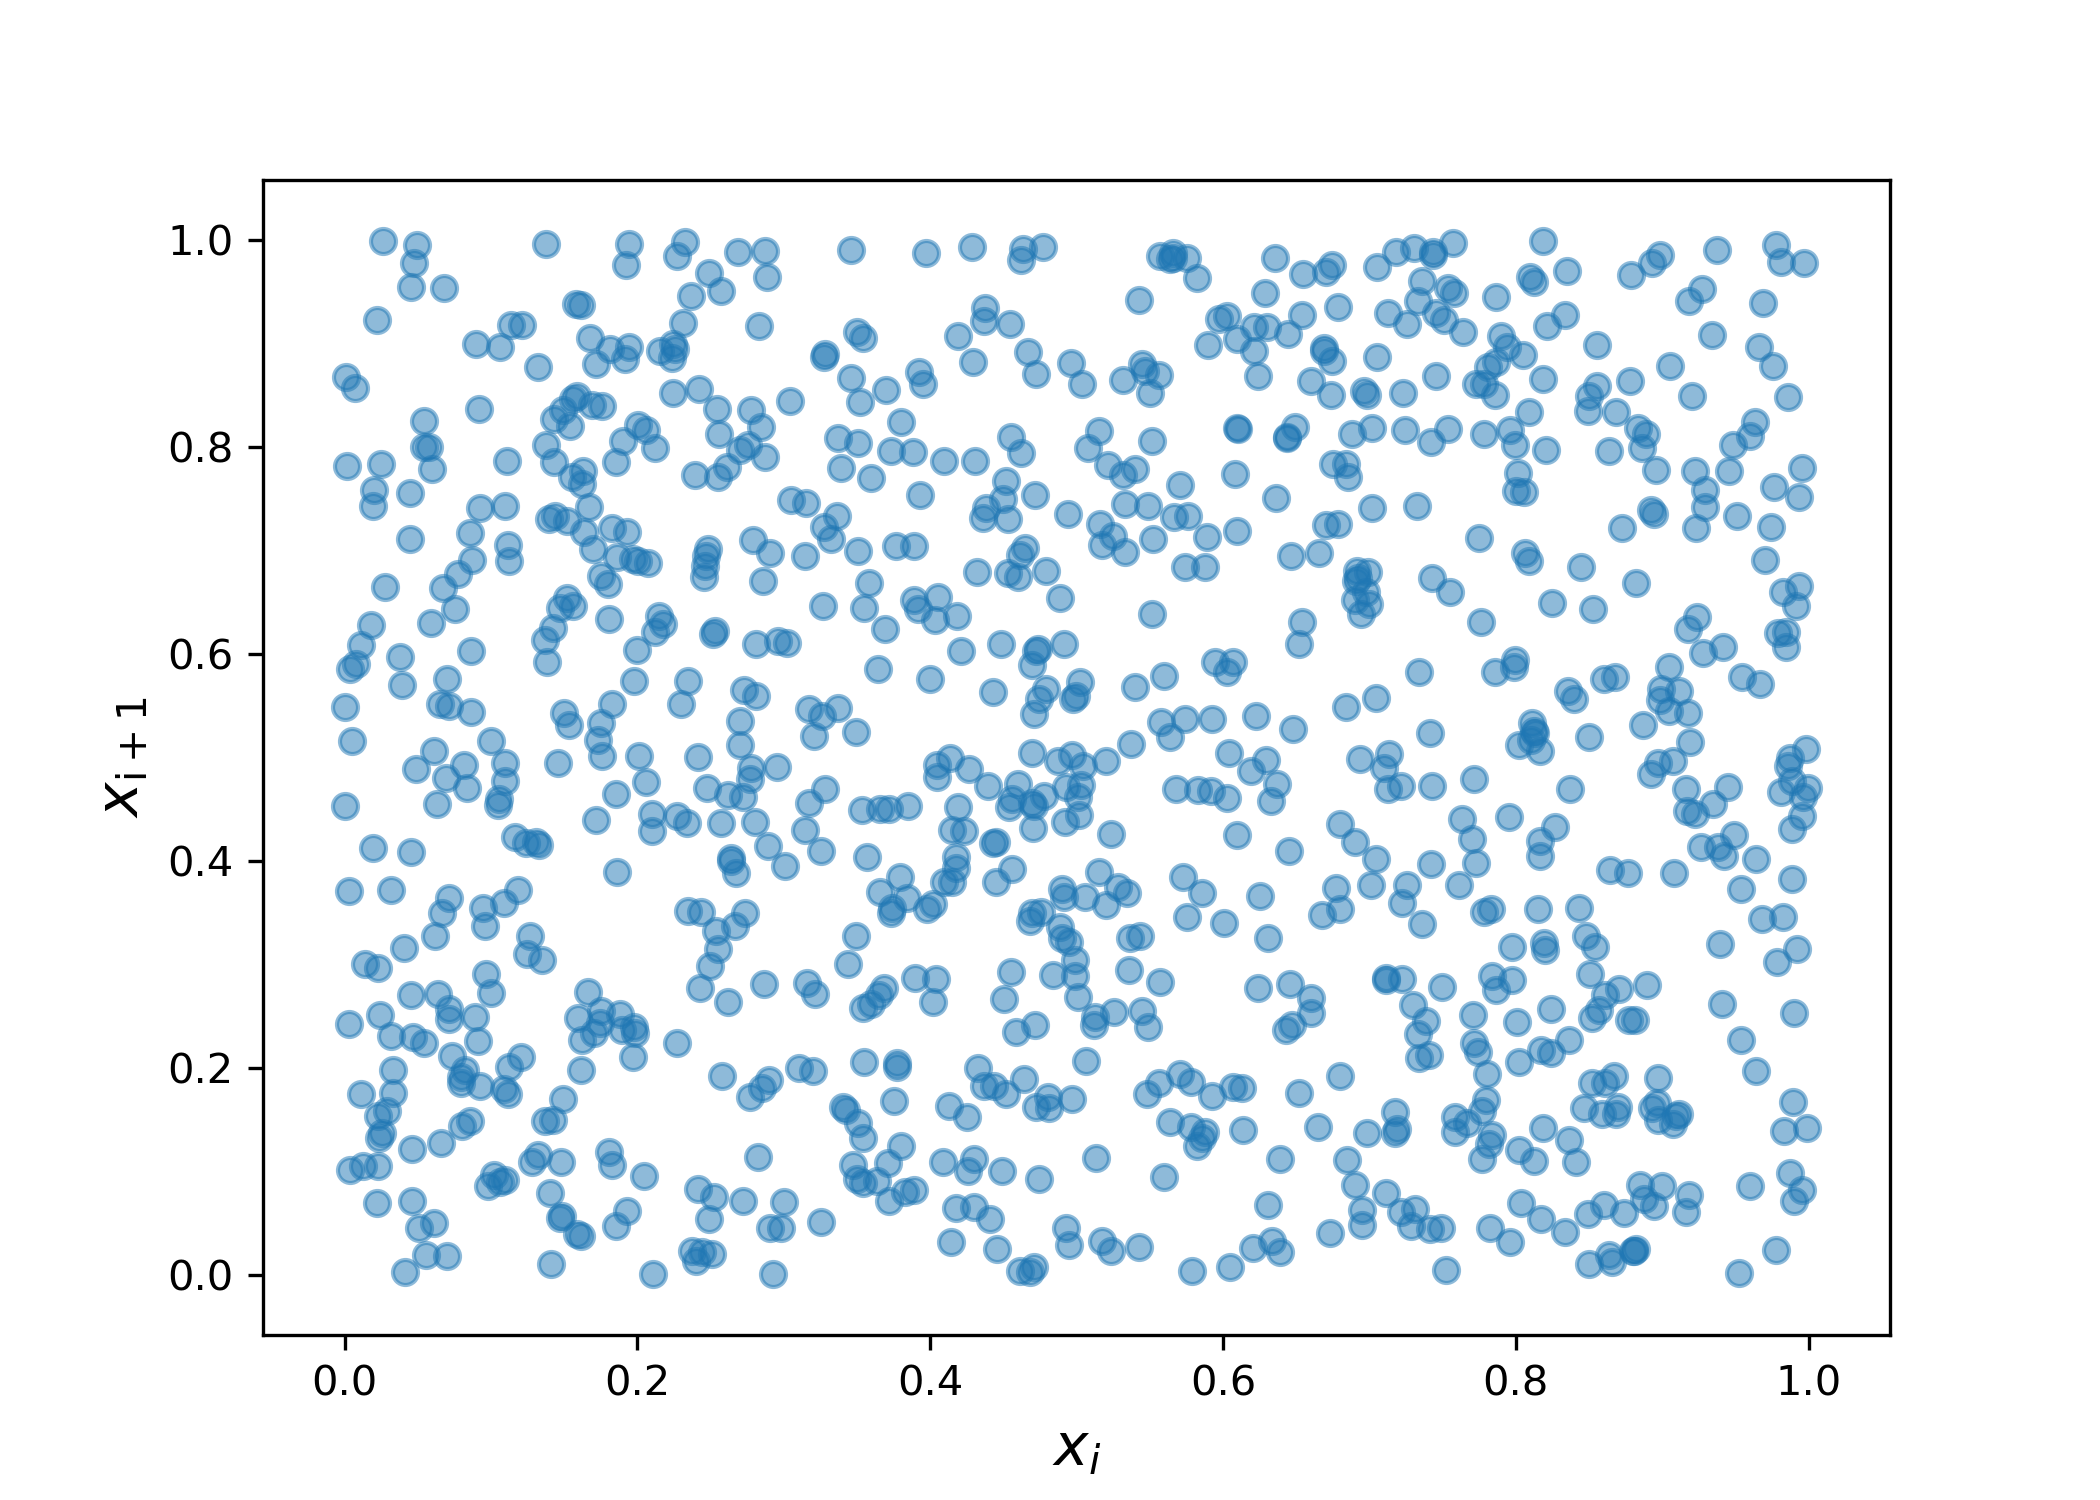
\includegraphics[width=0.9\linewidth]{./plots/x_x_1.png}
    \caption{$x$ vs. $x_{i+1}$ for the random number generator.}
    \label{plt1}
\end{figure}
Looking at the $i$ versus the $i+1$ components of our rng, there appears
to be little correlation between the numbers, which is a good sign. In
\autoref{plt2} we see the values that each number has in the array of 
$1000$ random numbers. It is between $0$ and $1$, also a good sign.
\begin{figure}[h!]
    \centering
    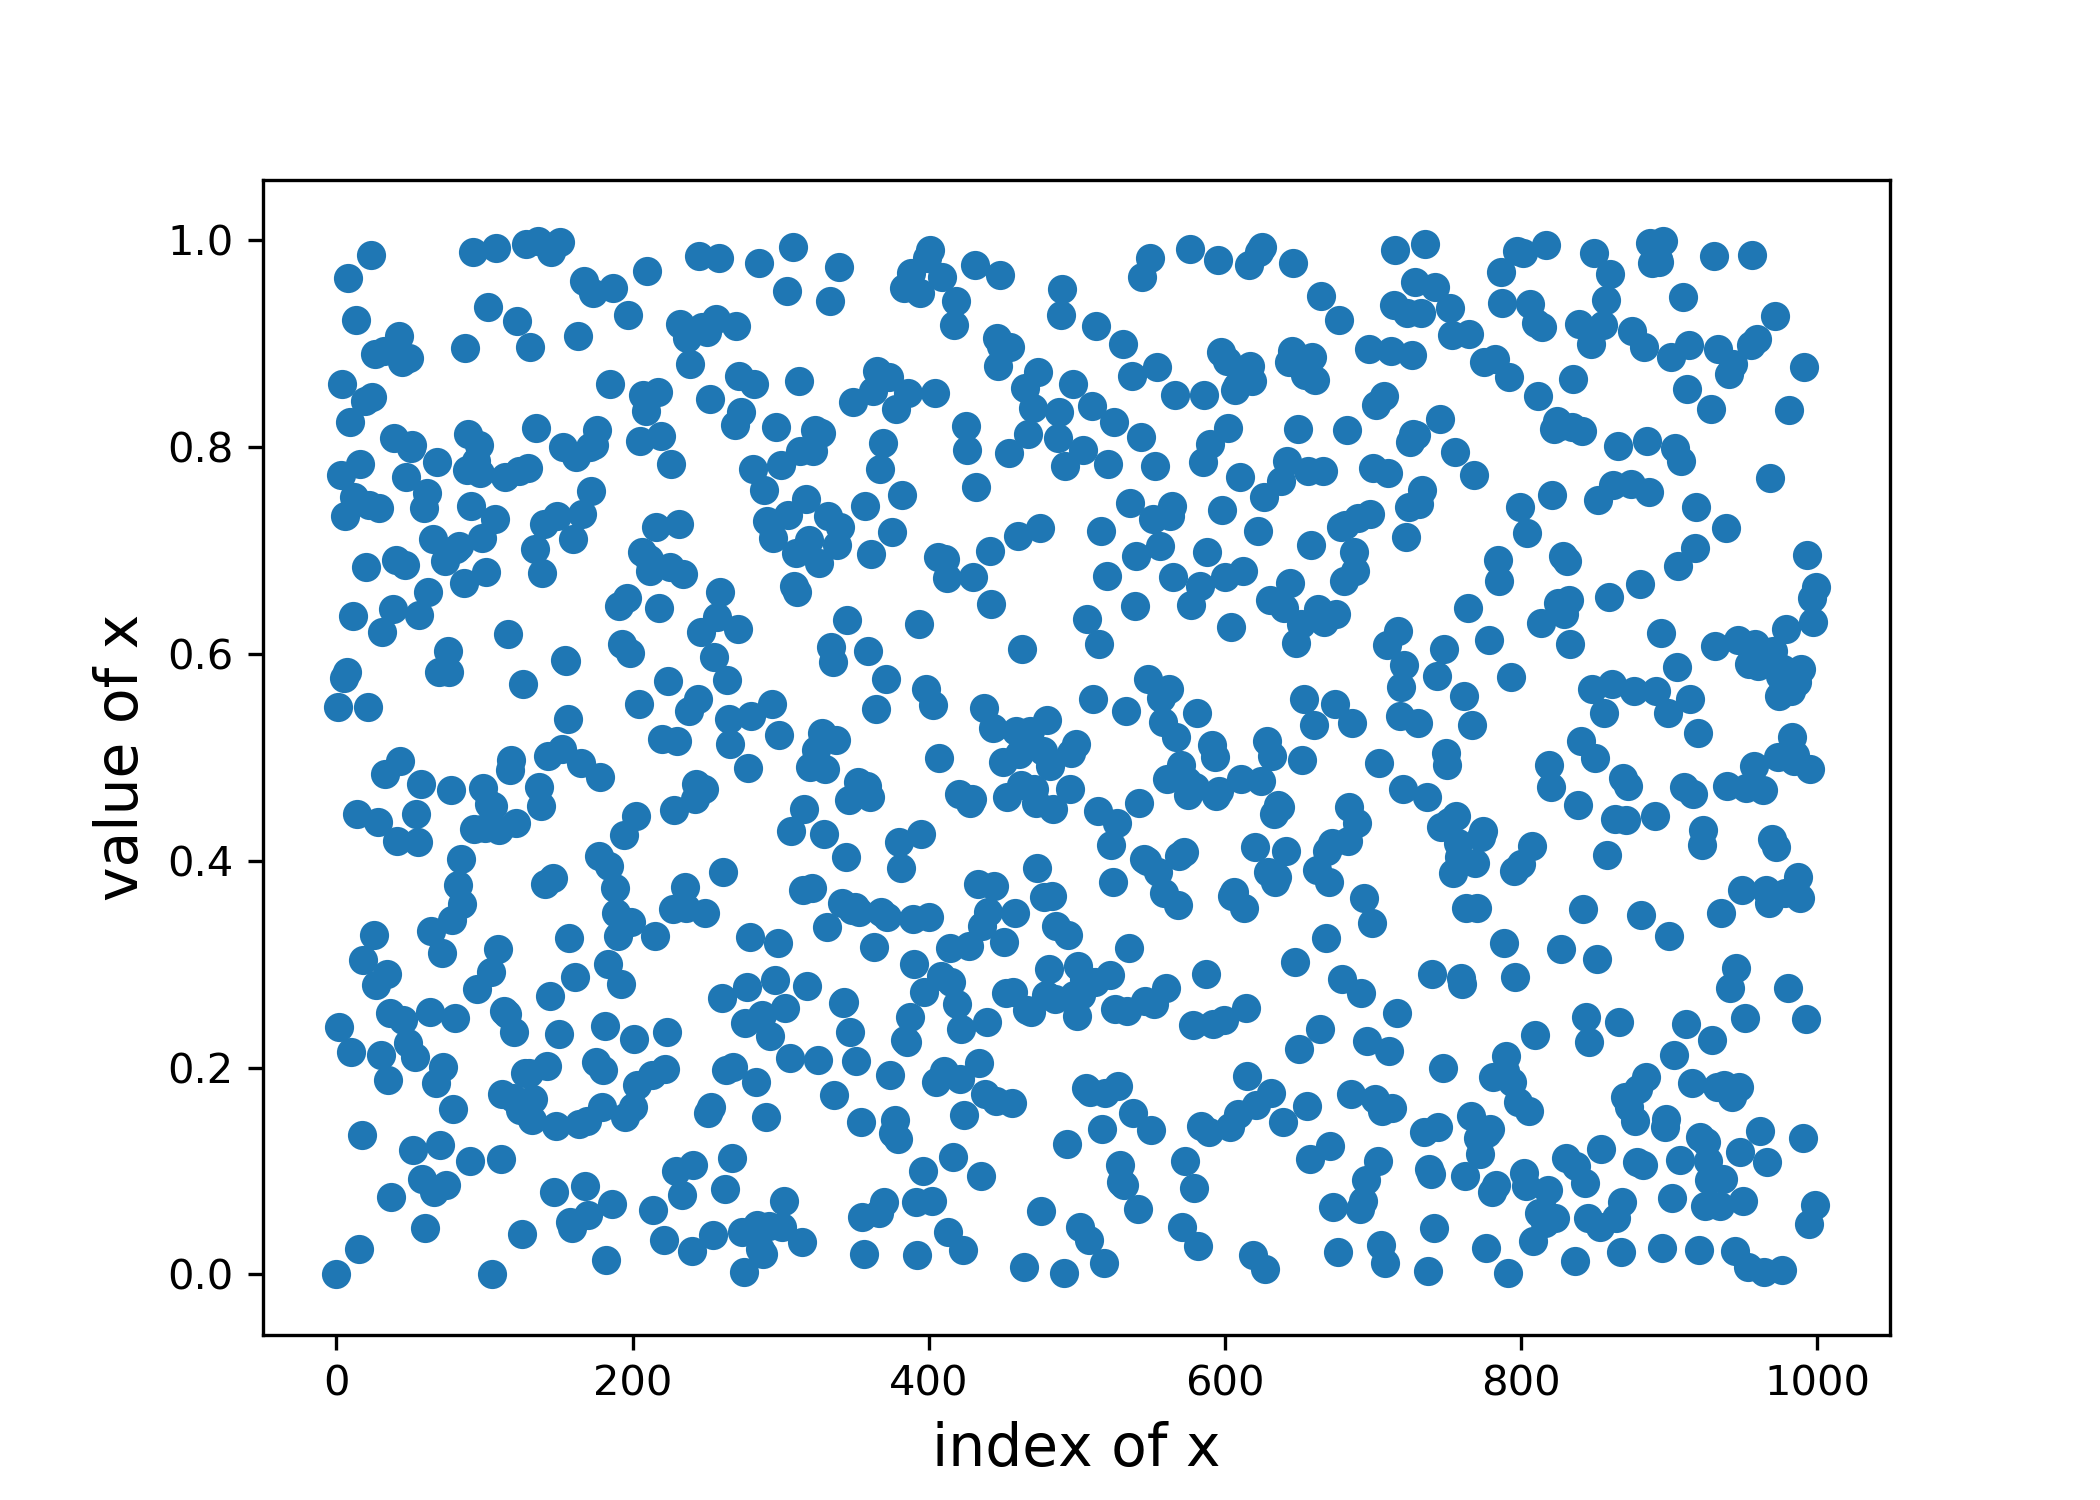
\includegraphics[width=0.9\linewidth]{./plots/xval_xind.png}
    \caption{The value of $x$ at a given index.}
    \label{plt2}
\end{figure}
However, in \autoref{plt3} it is clear something is wrong with the rng.
\begin{figure}[h!]
    \centering
    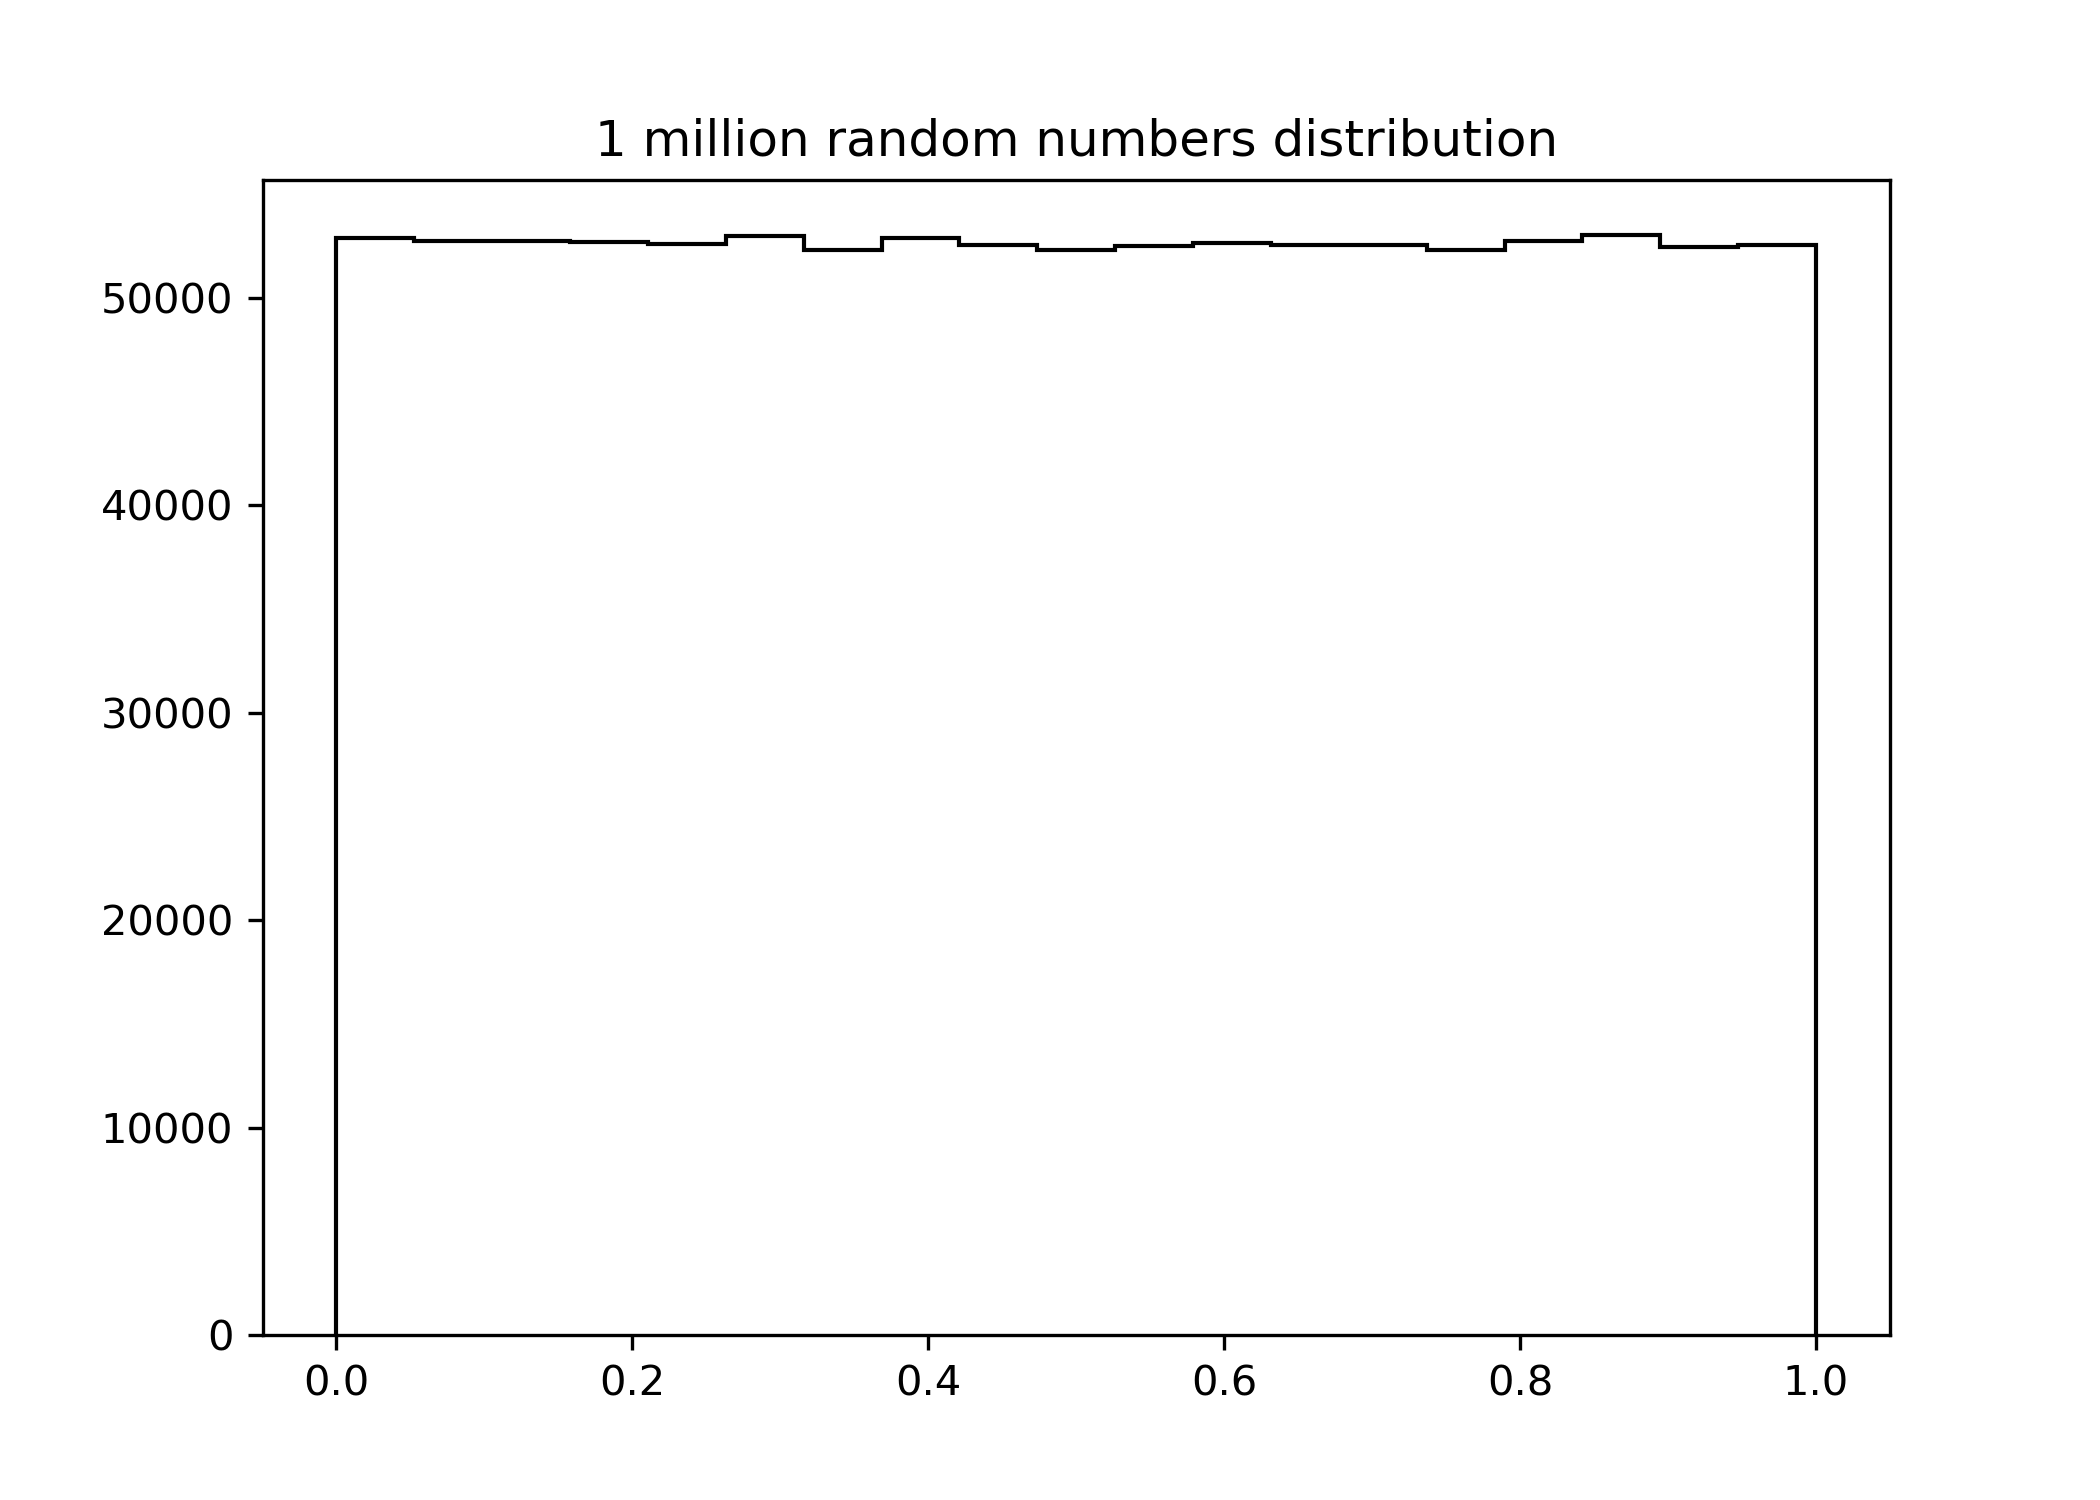
\includegraphics[width=0.9\linewidth]{./plots/1mil_hist.png}
    \caption{$1$ million random numbers plotted.}
    \label{plt3}
\end{figure}
As is plainly seen, the numbers in the random generator nearly all go above 
$5 \times 10^4$, which is not what we would expect from the rng. I am not
sure what the issue is. I attempted to cast all of the values as \texttt{ints}
but I was getting runtime errors in the $XOR$ bit-shift. The variance appears
to be fine, so I left it as is.


\subsection{1b}

\lstinputlisting{p1b.py}

As I have already explained that my rng is likely wrong, I will not mention
it further in the exercise. Here we use the Box-Muller method to generate
a Gaussian distribution, seen in \autoref{plt4}.
\begin{figure}[h!]
    \centering
    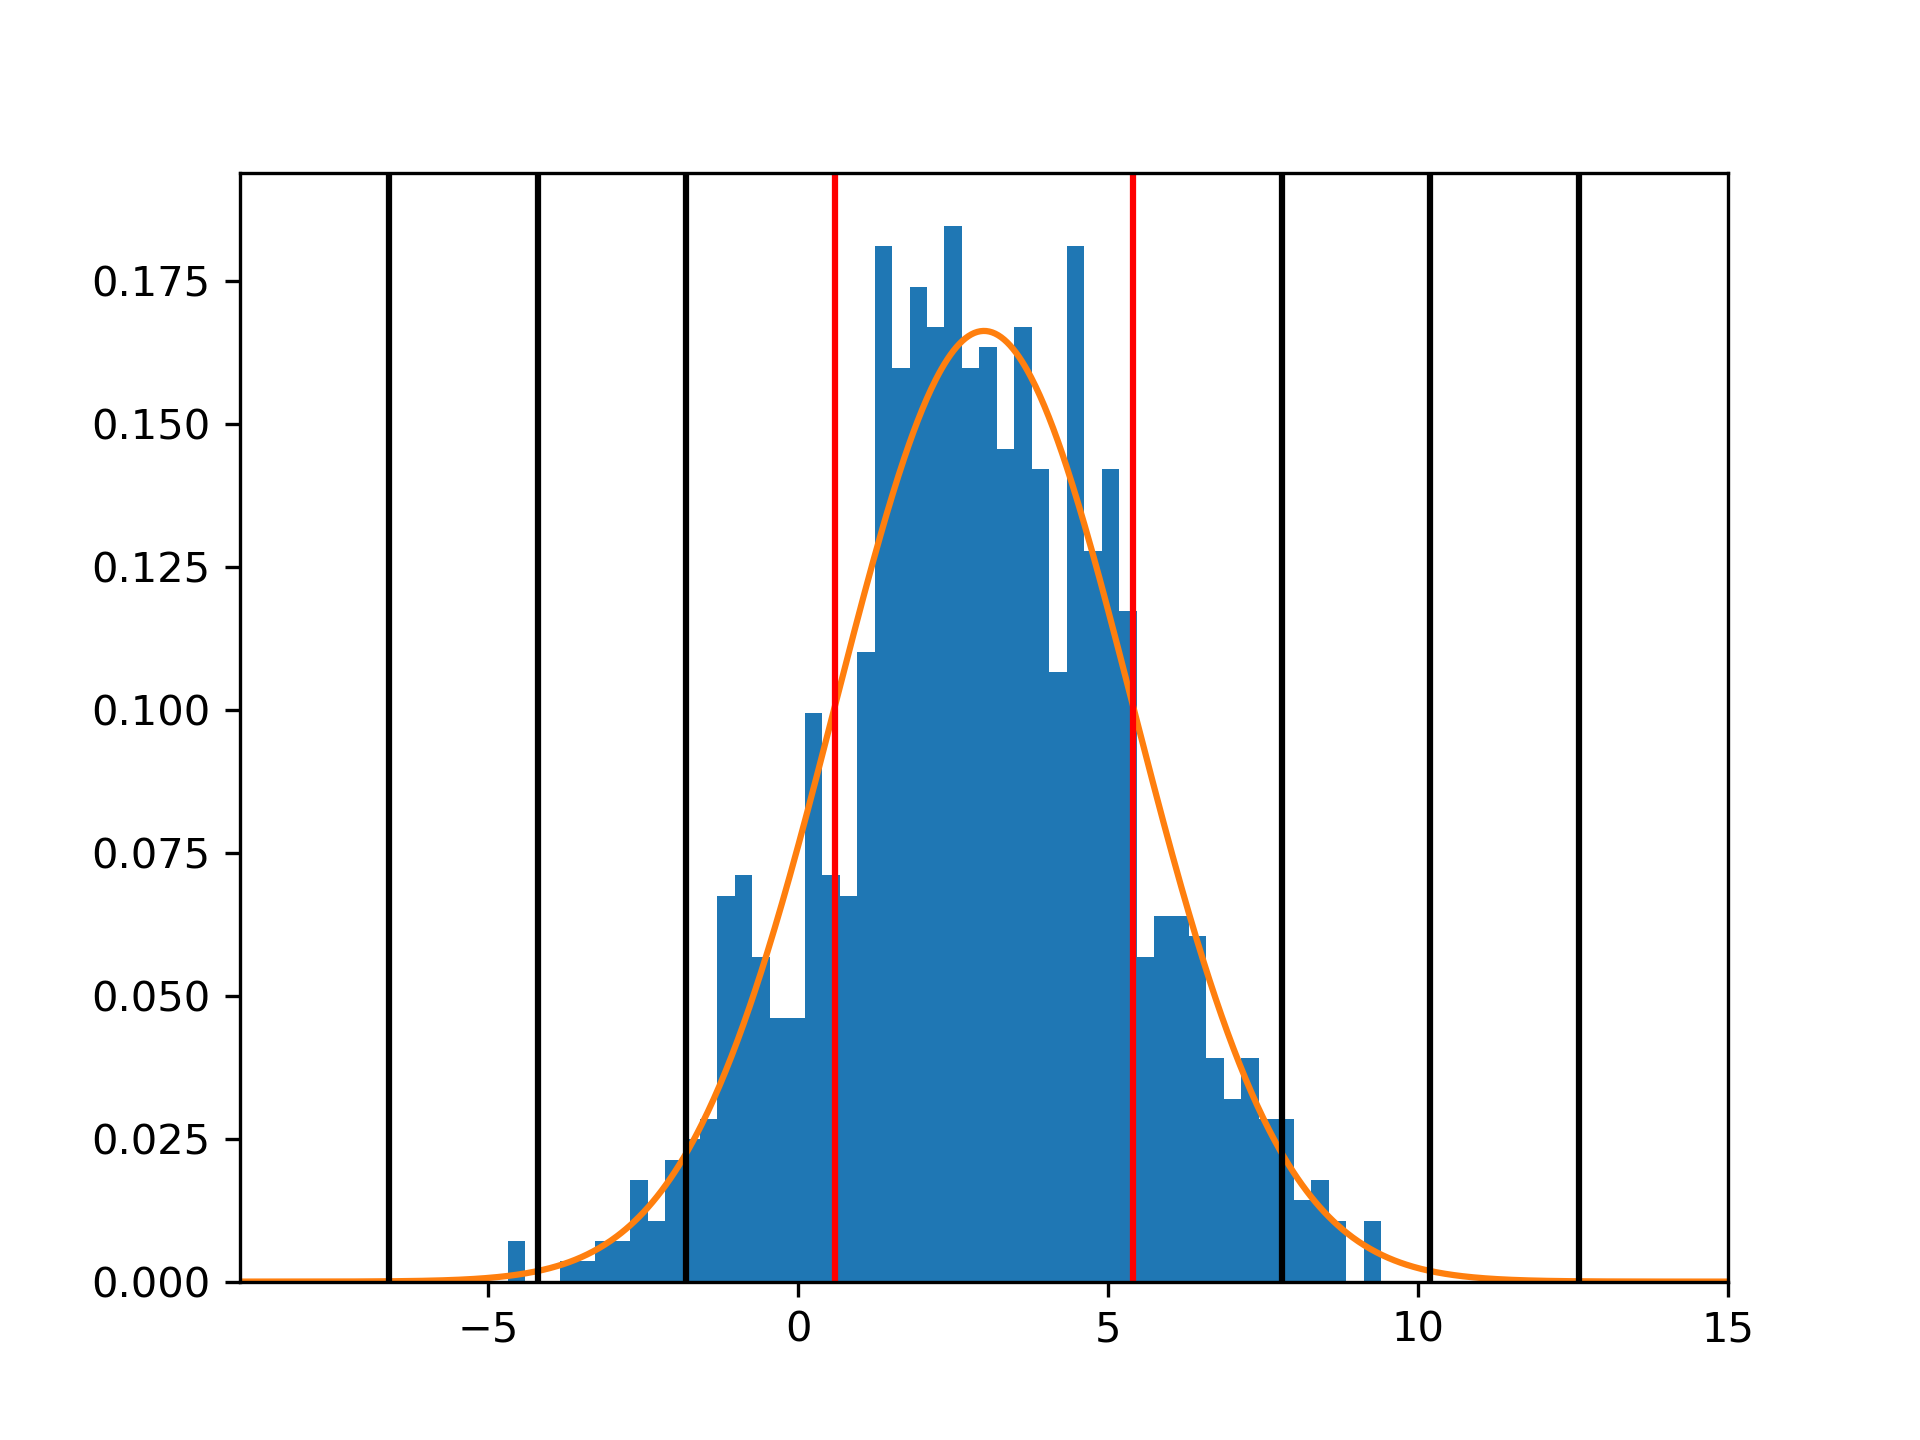
\includegraphics[width=0.9\linewidth]{./plots/box_gauss.png}
    \caption{My distribution with \texttt{numpy.norm} overplotted.}
    \label{plt4}
\end{figure}
The Box-Mueller method seems to work nicely, it is simply the rng that
ruins the Gaussian, given that there are values that are favored in the
$+1\sigma$ range.


\subsection{1c}

\lstinputlisting{p1c.py}
Next is the KS test. For this, I am unsure where I went wrong because
I followed the slides but to no avail. With time constraints, I was not
able to figure it out. Figures are plotted below.
\begin{figure}[h!]
    \centering
    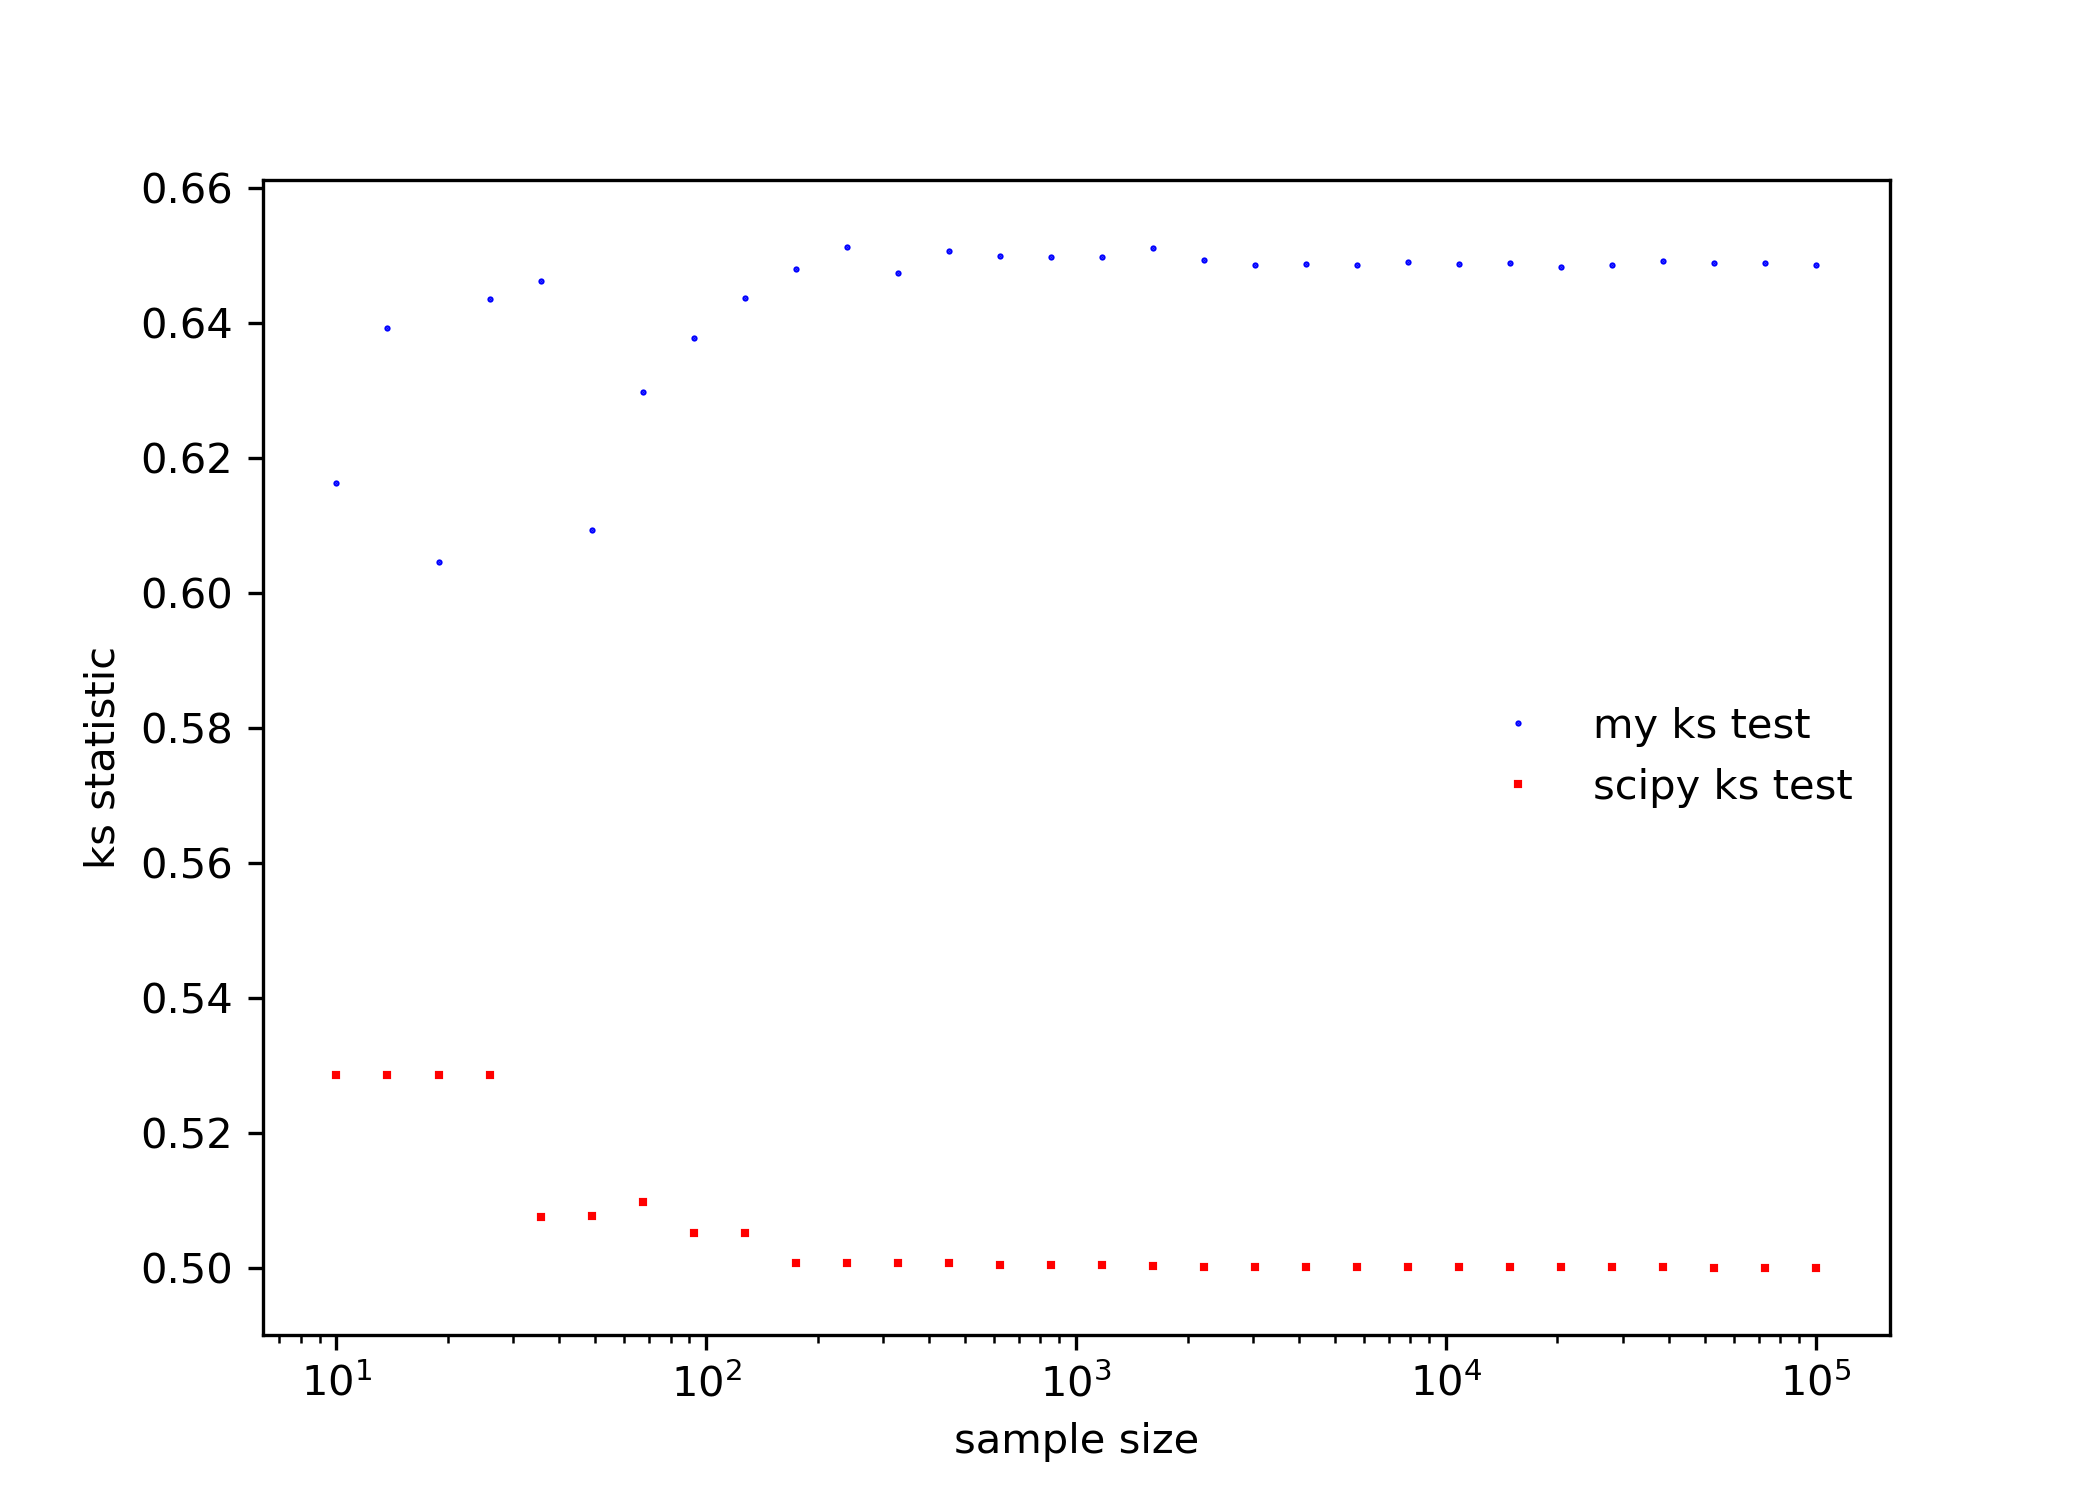
\includegraphics[width=0.9\linewidth]{./plots/ks_stat.png}
    \caption{$1$ million random numbers plotted.}
    \label{plt3}
\end{figure}

\begin{figure}[h!]
    \centering
    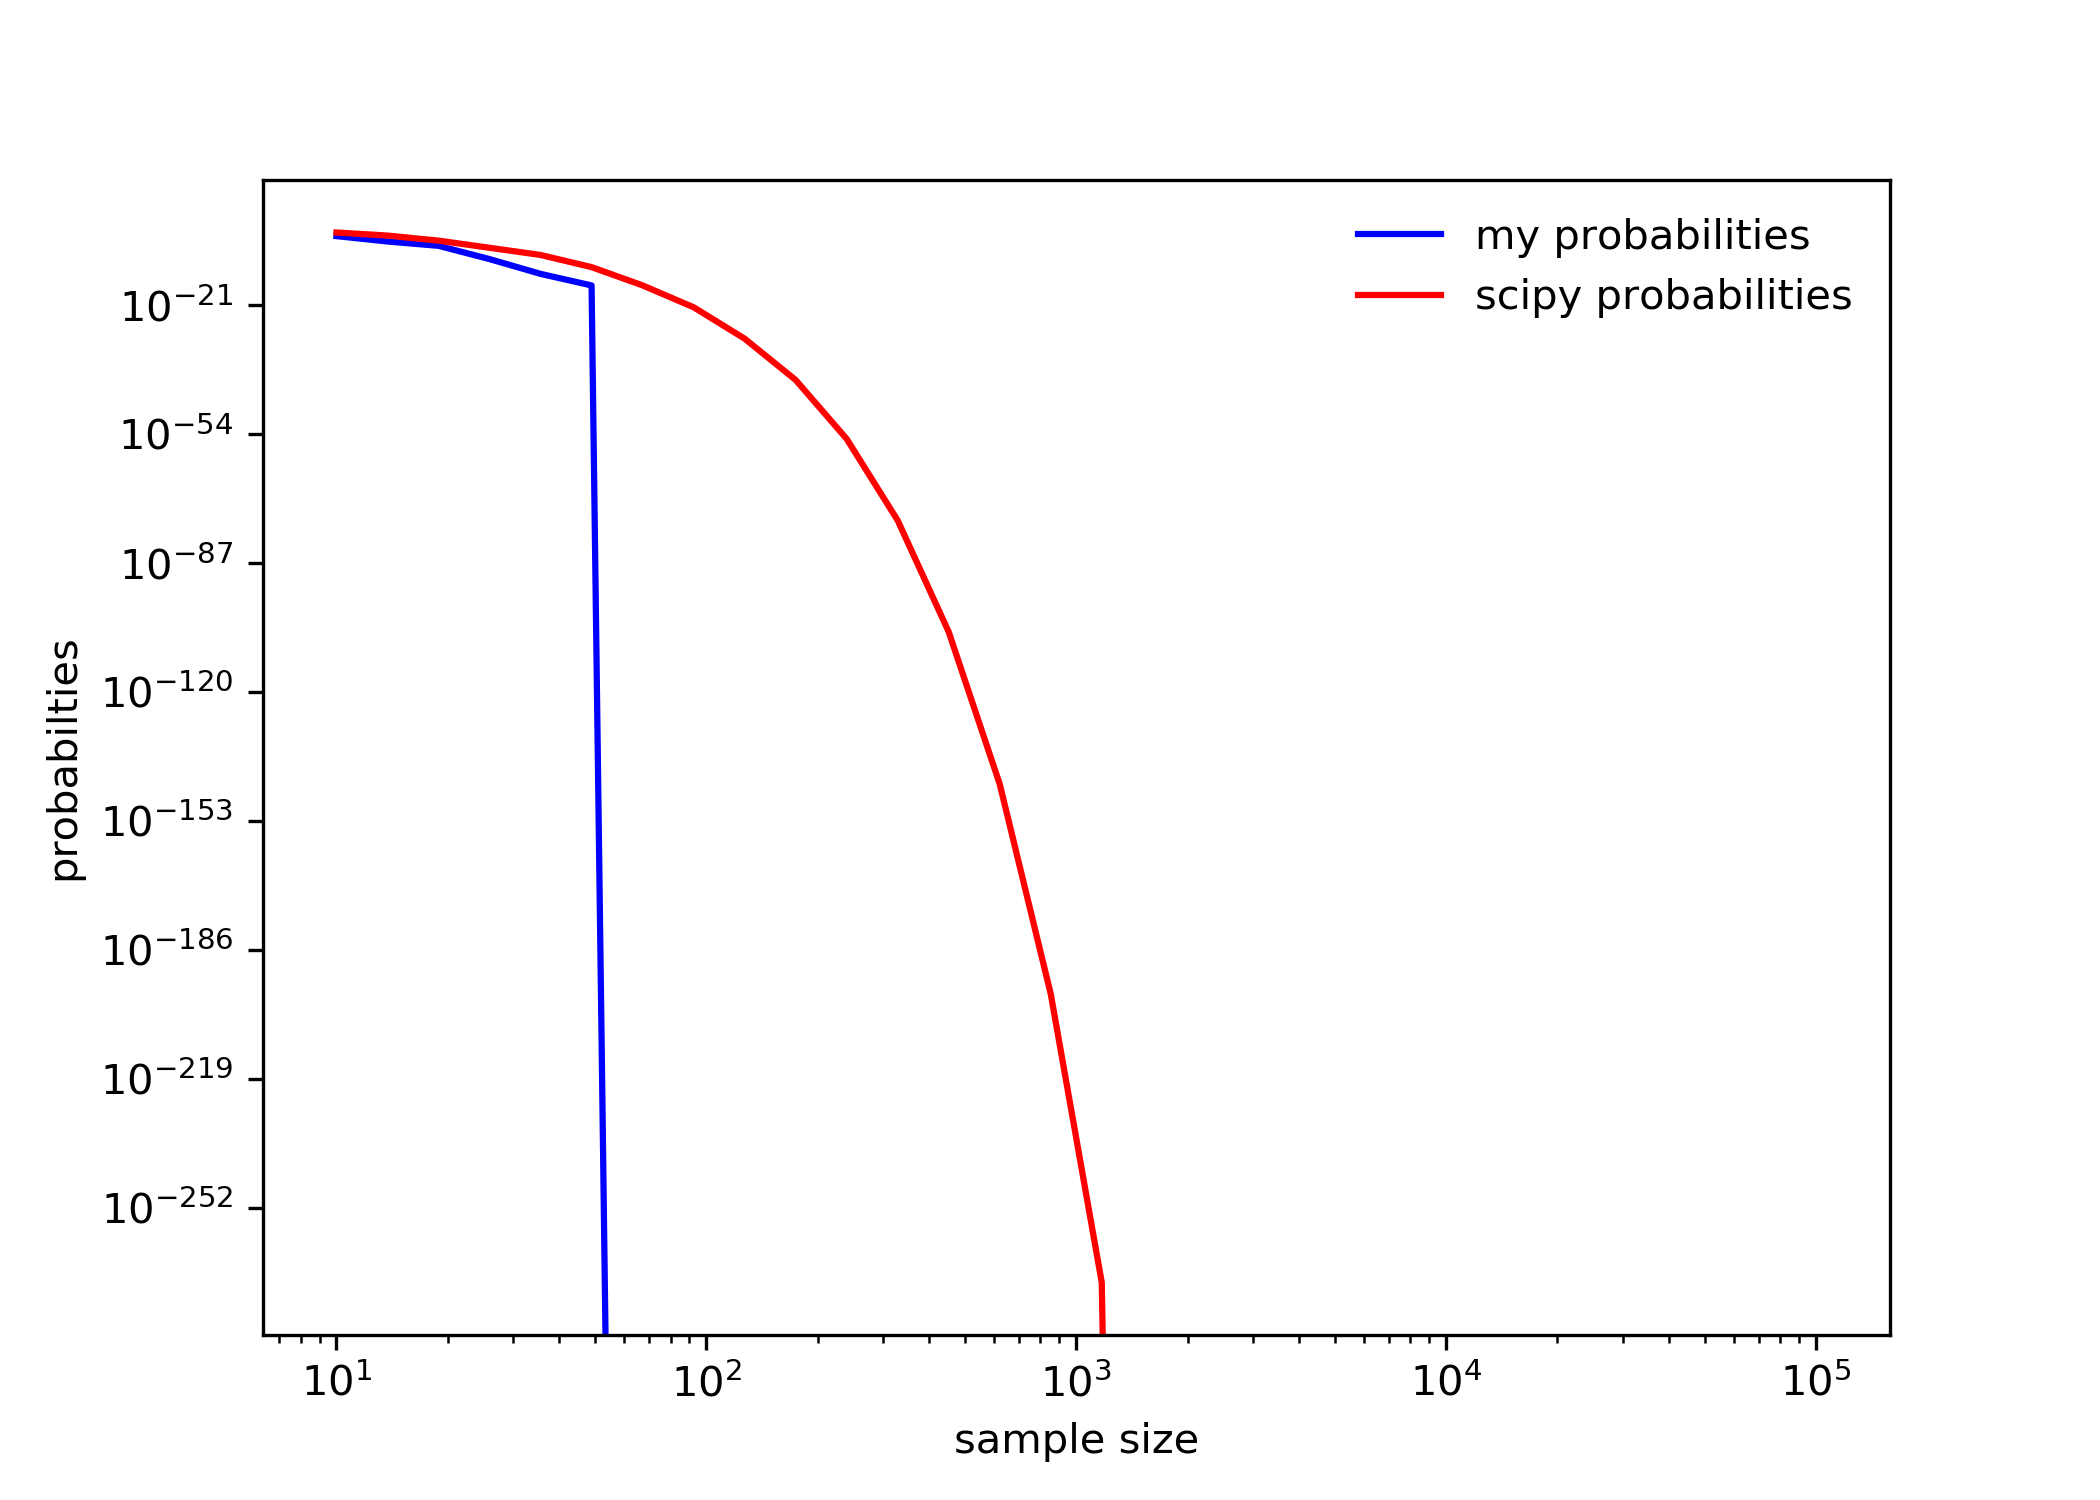
\includegraphics[width=0.9\linewidth]{./plots/ks_prob.png}
    \caption{$1$ million random numbers plotted.}
    \label{plt3}
\end{figure}



\subsection{1d}

\lstinputlisting{p1d.py}
Next is the Kuiper test. As with the KS test, I am unsure where I went wrong
because I followed the slides but to no avail. With time constraints, 
I was not able to figure it out. Figures are plotted below. One obvious 
explanation is that my distribution does not fit a Gaussian.
I am unsure of potential (and likely) bugs in my code.
\begin{figure}[h!]
    \centering
    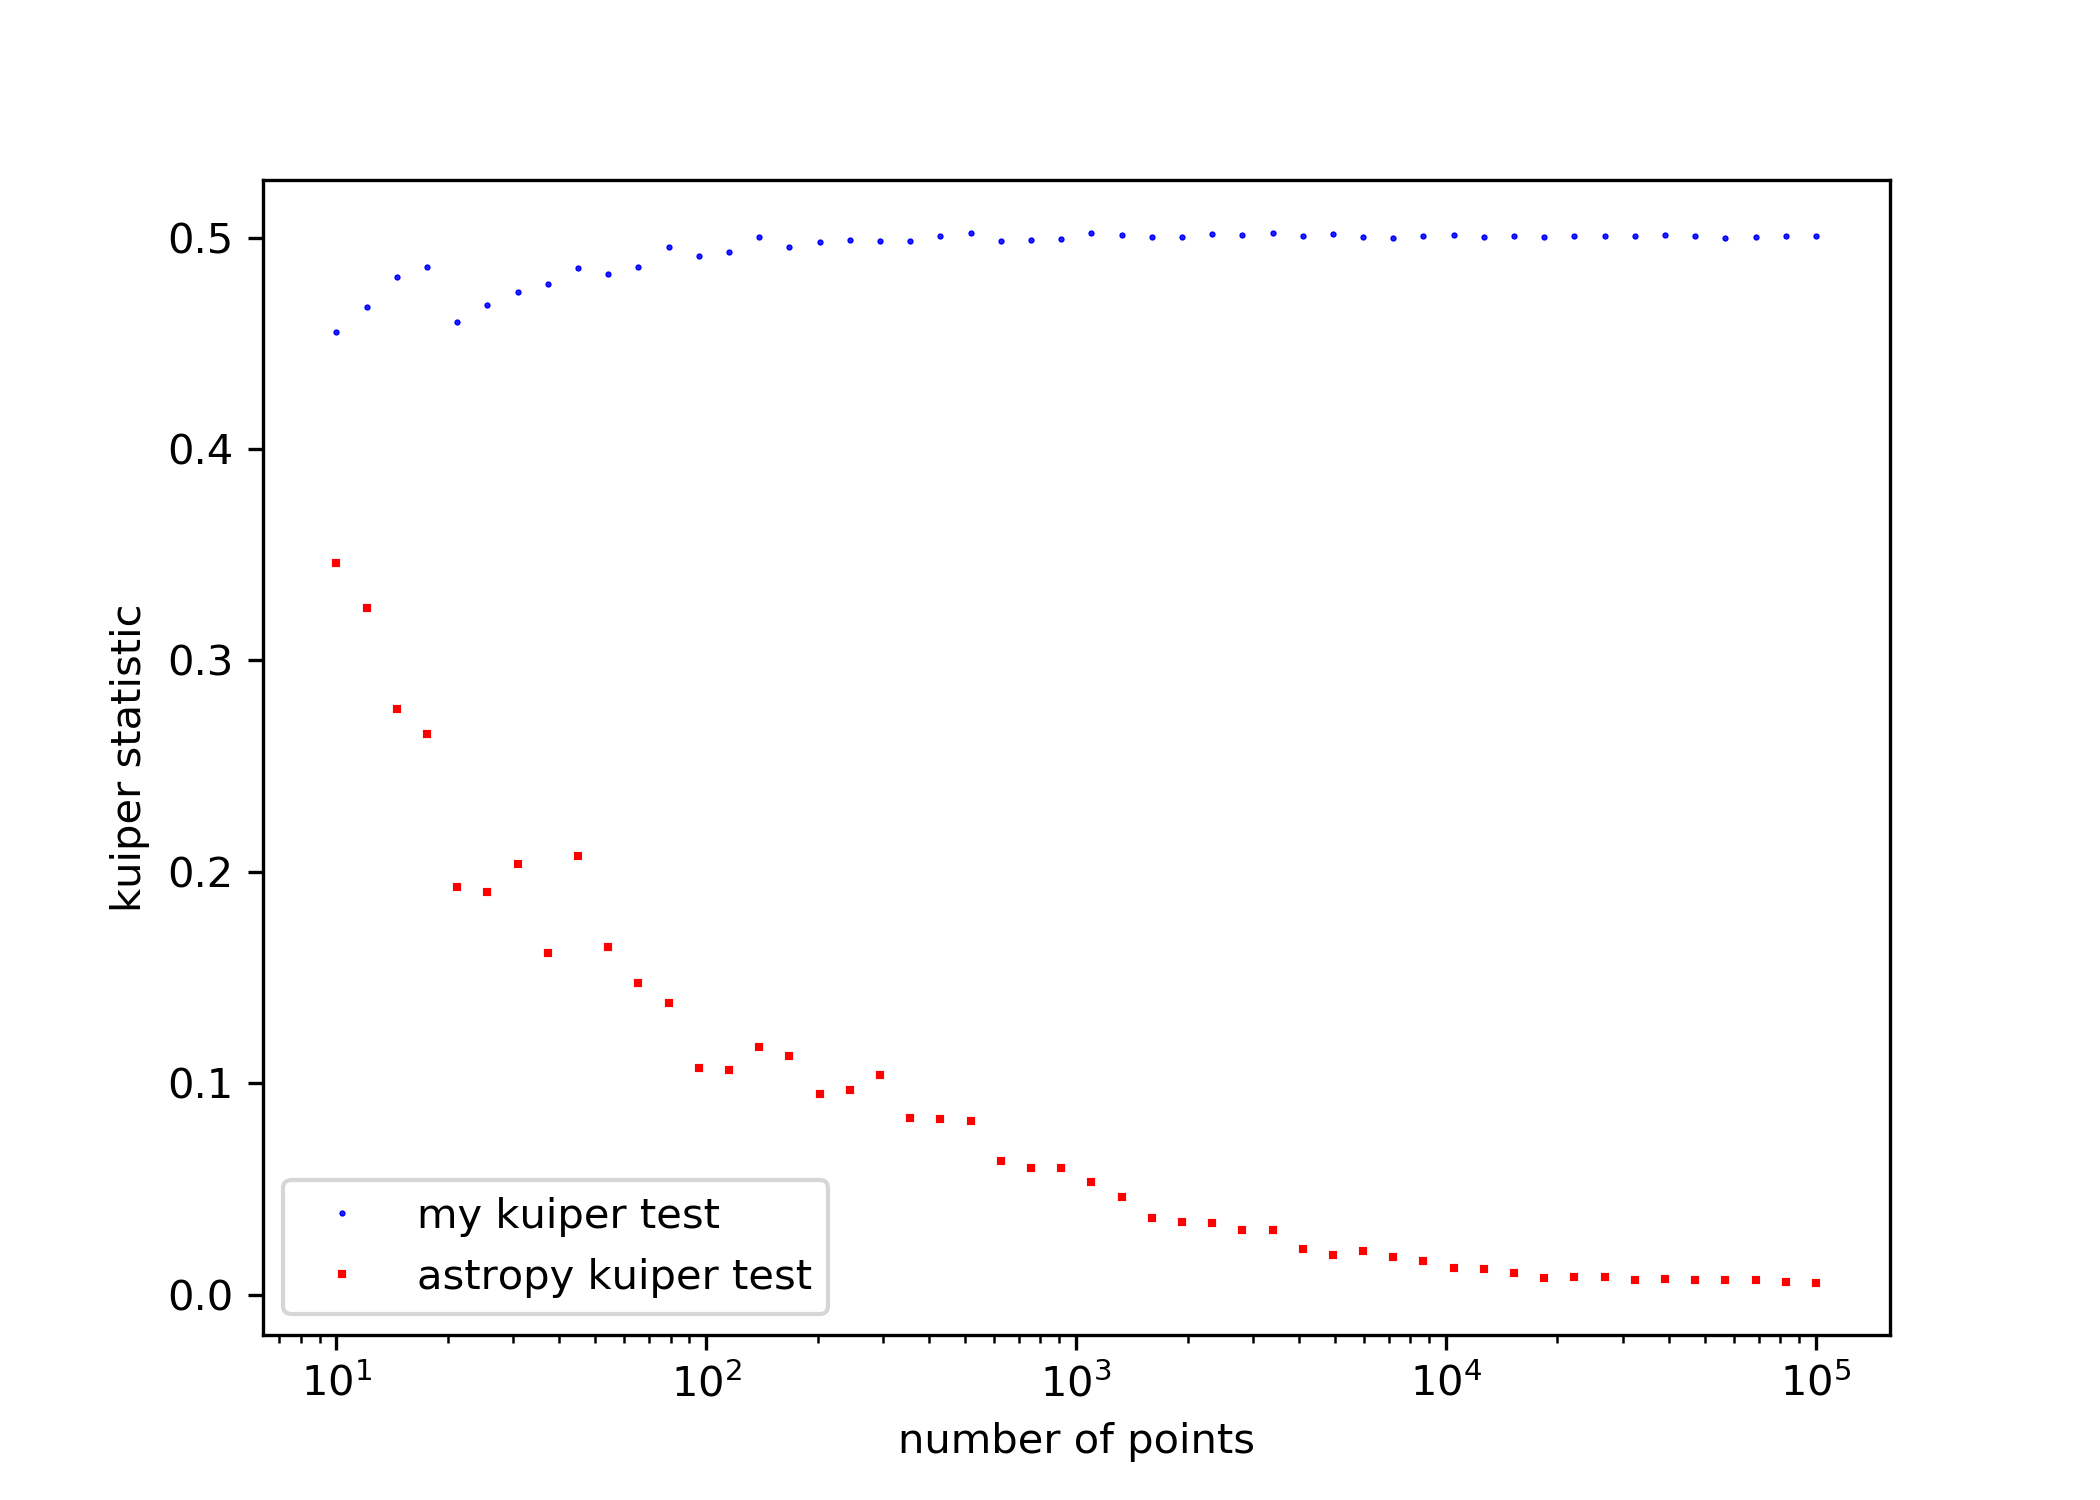
\includegraphics[width=0.9\linewidth]{./plots/kuiper_stat.png}
    \caption{Kuiper distance statistic.}
    \label{kuip_s}
\end{figure}

\begin{figure}[h!]
    \centering
    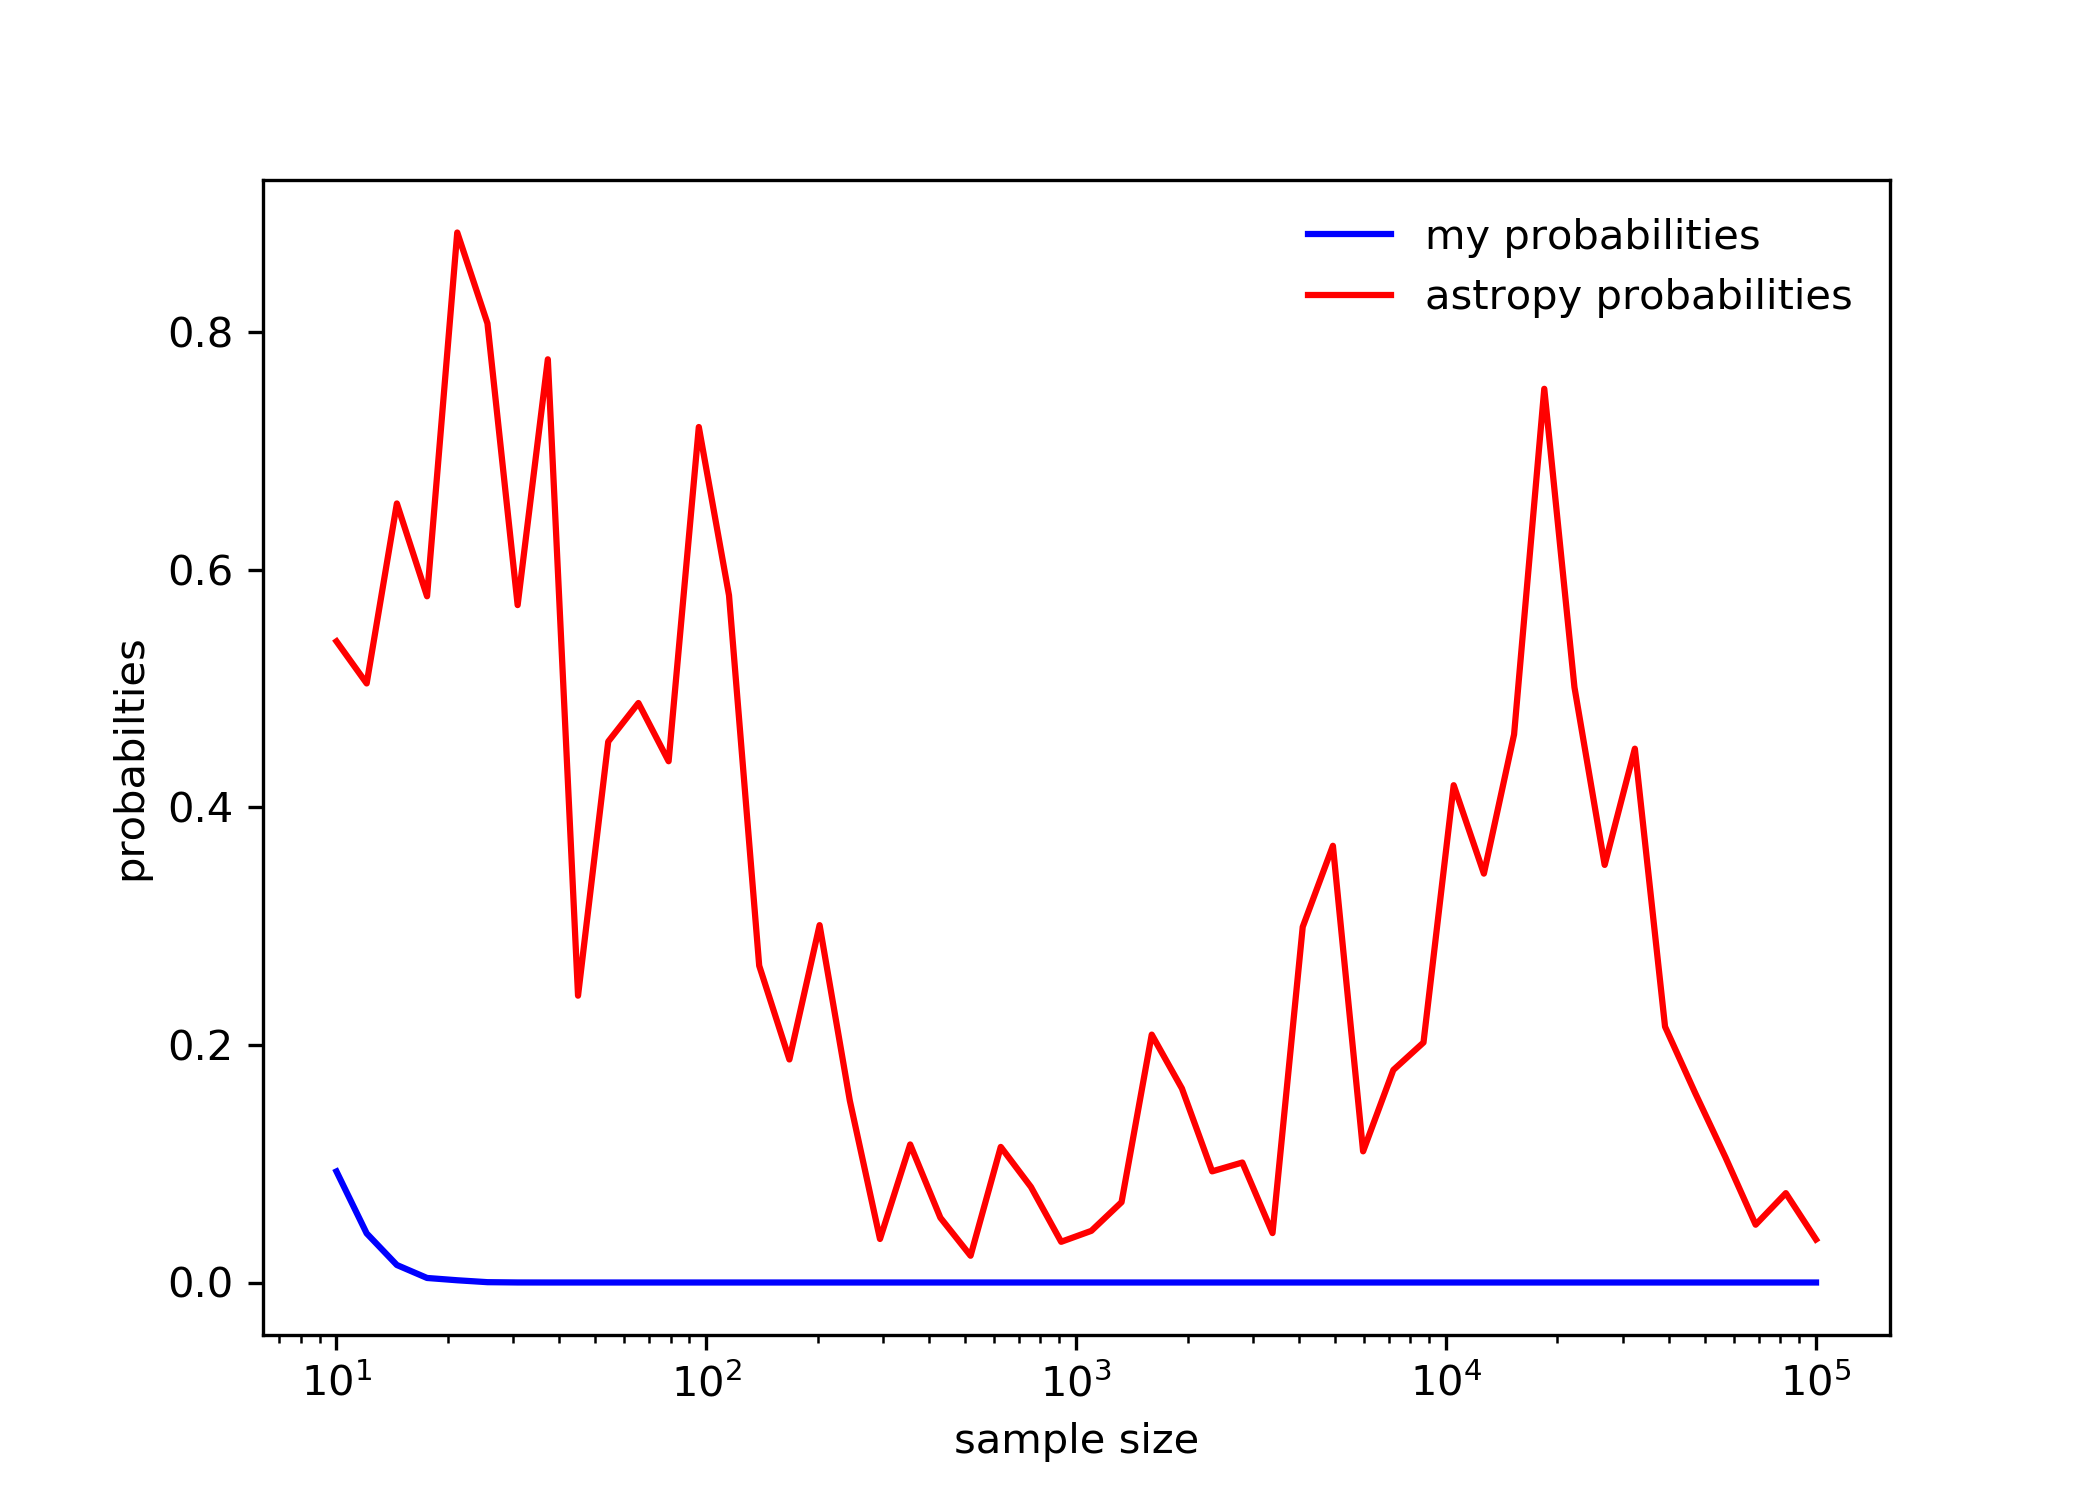
\includegraphics[width=0.9\linewidth]{./plots/k_prob.png}
    \caption{Kuiper probabilities.}
    \label{kuip_p}
\end{figure}



\subsection{1e}

\lstinputlisting{p1e.py}
Next, we are meant to verify a statistic of our choice (in this case the 
KS statistic) with a set of random numbers. I recognized too late that I need
to implement a $2$D KS sampler. As can be seen, I have a potential CDF to use,
but the statistic cannot be used at this time.



\section{Problem 2}

\lstinputlisting{p2.py}
We set out to make initial density fields based off of the power spectrum,
\begin{equation}
  P(k) = k^n,
\end{equation}
where $n$ is $-1, -2, -3$. Essentially, we setup the indices for the Fast
Fourier Transform (FFT) as described in the slides. We define the function
for the power spectrum, use our rng to make random numbers, and finally
perform the FFT on each field. Figures are plotted below.

\begin{figure}[h!]
    \centering
    \includegraphics[width=0.9\linewidth]{./plots/gauss_field_n_1.png}
    \caption{Gaussian field for $n=-1$.}
    \label{gf1}
\end{figure}
The initial field in \autoref{gf1} looks roughly what we expect.
Admittedly, I am unsure exactly what is expected, but as the handout
explains, dispersion is dependent on $n$. In \autoref{gf2} we can see
the dispersion causes a bit more ``clumpiness'' (that is, high-density
pockets). In \autoref{gf3}, we see an even higher contrast between
the low-high density regions. (Sorry, my colorbar was not working! It's 
viridis colormap, though.)
\begin{figure}[h!]
    \centering
    \includegraphics[width=0.9\linewidth]{./plots/gauss_field_n_2.png}
    \caption{Gaussian field for $n=-2$.}
    \label{gf2}
\end{figure}
However, in \autoref{gf3} it is clear something is wrong. The physical
distances are not changing as a function of $n$. As $P_k$ changes from
$n=-1$ to $n=-2$ for example, the maximum and minimum k values should increase
from $n=-1$ to $n=-2$. The physical distances should be larger as well.
Given time constraints, I gave up and left the plots as is. I assume 
it has a $2$-fold issue: my rng and perhaps the amplitudes are not actually
changing as expected.
\begin{figure}[h!]
    \centering
    \includegraphics[width=0.9\linewidth]{./plots/gauss_field_n_3.png}
    \caption{Gaussian field for $n=-3$.}
    \label{gf3}
\end{figure}



\section{Problem 3}

\lstinputlisting{p3.py}
We set out to solve the given ordinary differential equation (ODE) given in
the handout. I have very little to show--I do not have the analytic solution,
and it is clear from \autoref{rk} that the solution is not correct. My attempt
was to decompose the second-order ODE to a first-order, then to use the
Runge-Kutta fourth-order algorithm to solve the ODE. Results are below.
I needed much more help than I sought out, I recognize that. But, it was also
important to try and do the rest of the assignment as well...

\begin{figure}[h!]
    \centering
    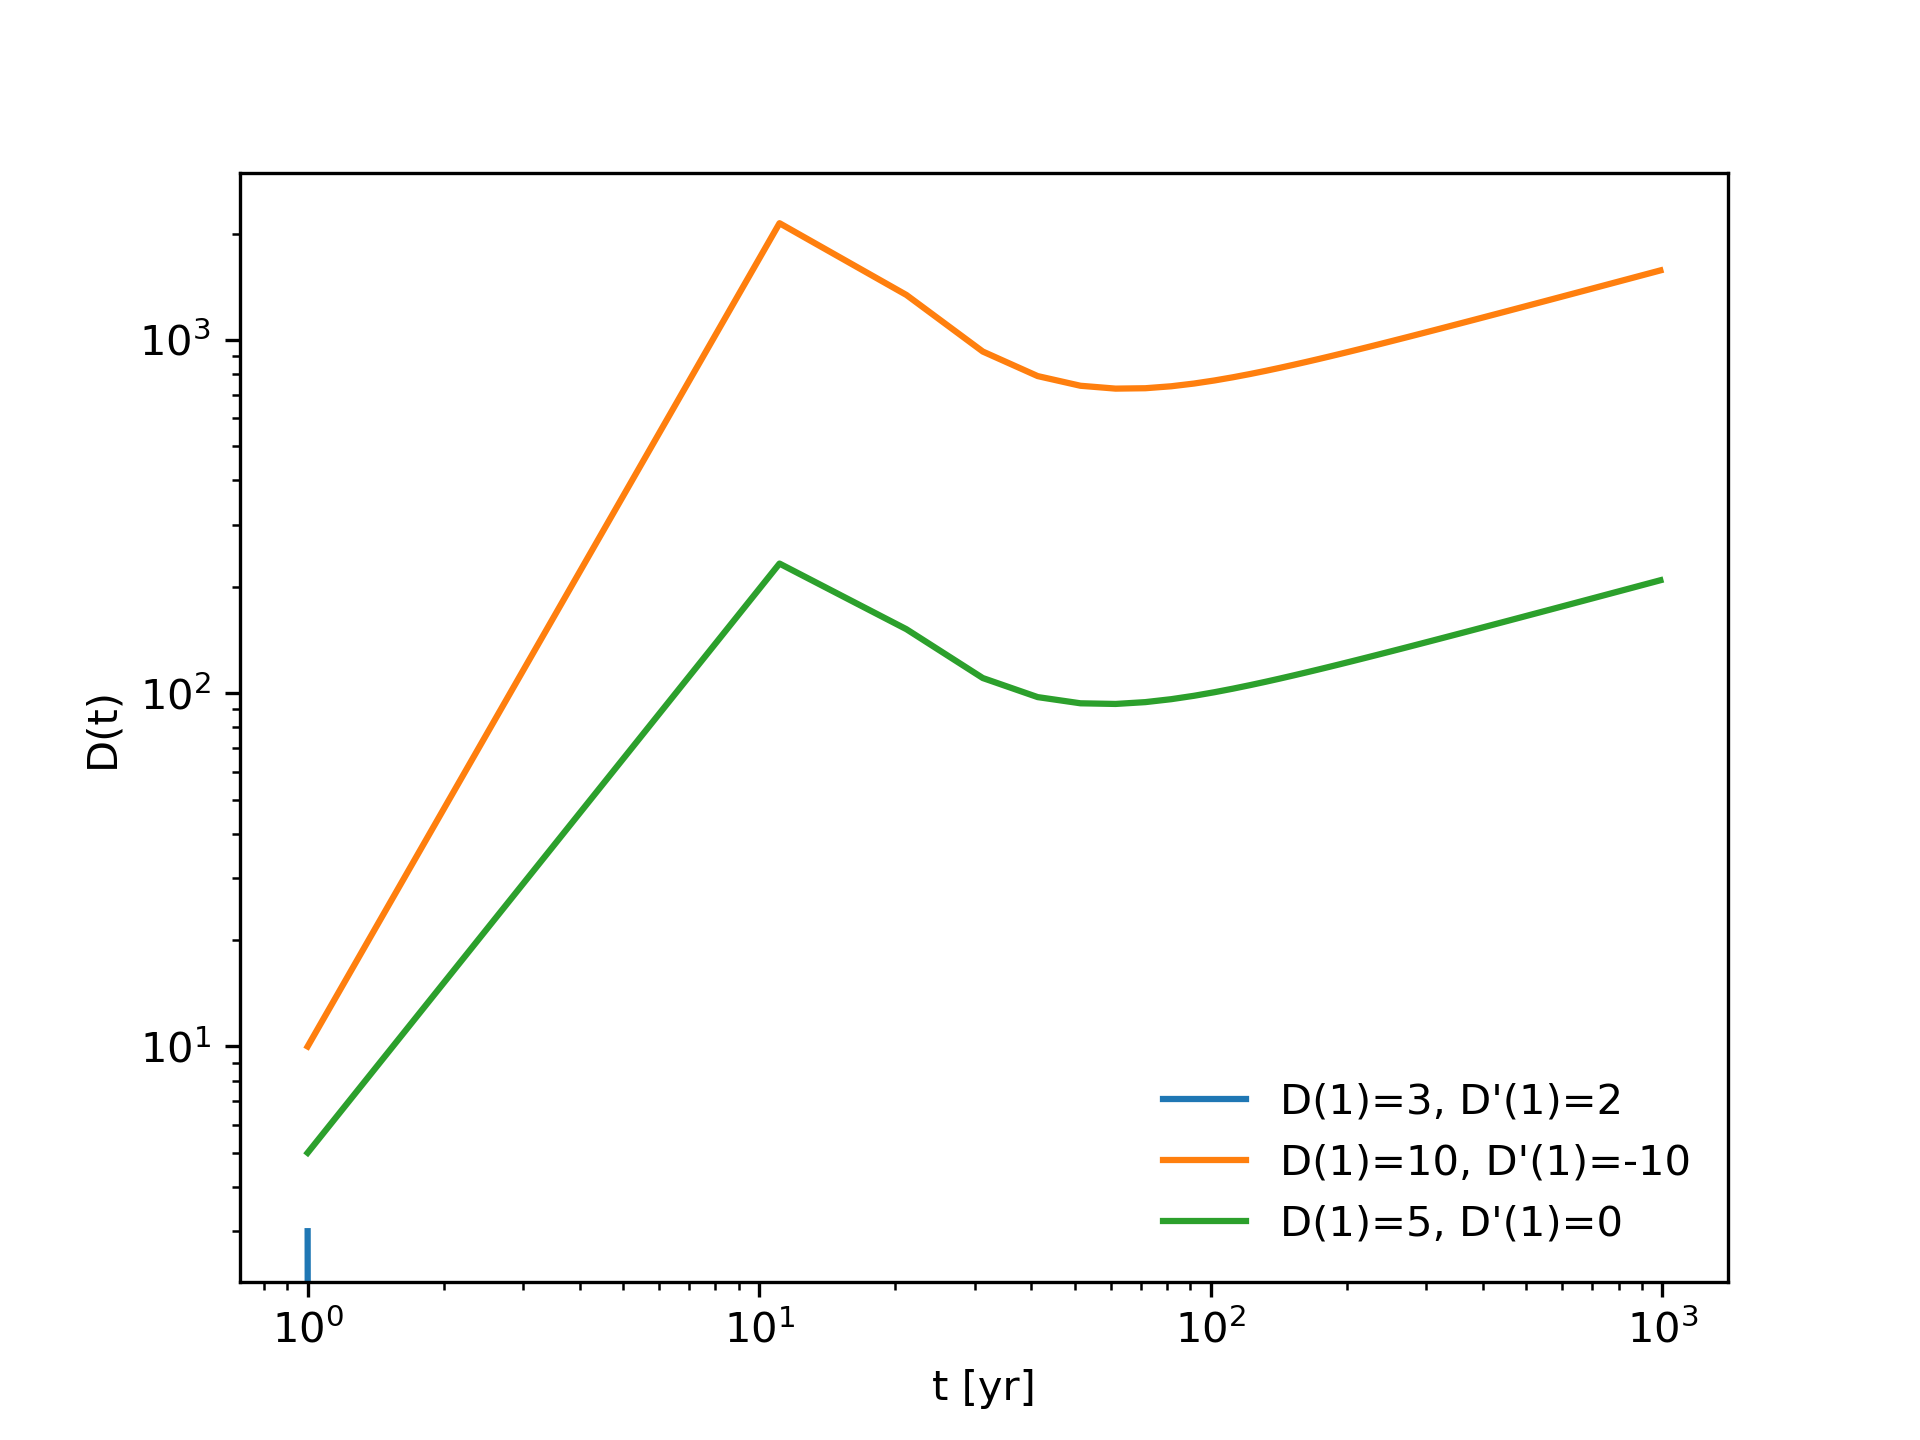
\includegraphics[width=0.9\linewidth]{./plots/rk4.png}
    \caption{Sad plot of the ODE solved.}
    \label{rk}
\end{figure}



\section{Problem 4}
\subsection{4a}

\lstinputlisting{p4a.py}
\lstinputlisting{p4a.txt}
We use the midpoint rule to calculate the desired integral. We achieve only
$1 \times 10^{-4}$ precision. We also use a bound that is sufficiently large
but is not actually $\inf$. A more robust integration is required to get
desired results.




\subsection{4b}

\lstinputlisting{p4b.py}
\lstinputlisting{p4b.txt}
We use the midpoint rule to calculate the desired integral again, but in terms
of the scale factor $a$. We give the value of the analytic derivative of the
linear growth factor at redshift $z=50$ ($a = \frac{1}{51}$),
\begin{equation}
 \dot D(t) = \frac{dD}{da}\dot a,
\end{equation}
using the integral we calculated numerically. The derivative is,
\begin{equation}
 \dot D(t) = \frac{-15}{4}\Omega_m^2 H_0 \frac{I}{a_{\textrm{f}}^3},
\end{equation}
where $\Omega_m$ is the matter density, $H_0$ the Hubble constant,
$a_{\textrm{f}}$ the final scale factor, and $I$ the integral given by,
\begin{equation}
 \int_{a=0}^{a=\frac{1}{51}} \frac{\frac{1}{a^3}}
   {\frac{\Omega_{\textrm{m}}{a^3} + \Omega_{\Lambda}}},
\end{equation}
where $\Omega_{\Lambda}$ is the cosmological constant.


\subsection{4b}

\lstinputlisting{p4b.py}
\lstinputlisting{p4b.txt}
We use the midpoint rule to calculate the desired integral again, but in terms
of the scale factor $a$. We give the value of the analytic derivative of the
linear growth factor at redshift $z=50$ ($a = \frac{1}{51}$),
\begin{equation}
 \dot D(t) = \frac{dD}{da}\dot a,
\end{equation}
using the integral we calculated numerically. The derivative is,
\begin{equation}
 \dot D(t) = \frac{-15}{4}\Omega_m^2 H_0 \frac{I}{a_{\textrm{f}}^3},
\end{equation}
where $\Omega_m$ is the matter density, $H_0$ the Hubble constant,
$a_{\textrm{f}}$ the final scale factor, and $I$ the integral given by,
\begin{equation}
 \int_{a=0}^{a=\frac{1}{51}} \frac{\frac{1}{a^3}}
   {\frac{\Omega_{\textrm{m}}{a^3} + \Omega_{\Lambda}}},
\end{equation}
where $\Omega_{\Lambda}$ is the cosmological constant.


\subsection{4c}
Not implemented. Sad!


\subsection{4d}
Not implemented. Sad!


\section{Problem 5}
\subsection{5a}


\subsection{5b}
Not implemented. Sad!


\subsection{5c}
Not implemented. Sad!

But, I think we use this method to achieve a more realistic picture of
possible interactions between particles.


\subsection{5d}
Not implemented. Sad!


\subsection{5e}
Not implemented. Sad!


\subsection{5f}
Not implemented. Sad!


\subsection{5b}
Not implemented. Sad!


\section{Problem 6}
\lstinputlisting{p6.py}
\lstinputlisting{p6.txt}
Another unfortunate result. After following the slides and a few YouTube
videos, this is what I was able to come up with: a couple linear regression
models. I had made a bit of a breakthrough in understanding $27/5/2019$,
a bit too late to spend enough time with it to make a nice, working
program though. The ``cost'' estimations (that is, the predicted values)
are not yet yielding what the problem asks for specifically.

However, I will say that I checked for correlations between the parameters
(uncomment the code if you are curious) and I have to note that it is a bit
unfair to give us an assignment wherein we implement logistic regression on
a dataset where the parameters are not even correlated with each other.
Especially given that it is likely none of us have ever implemented machine
learning algorithms before. It makes it that much more difficult to figure out
what to even do.


\section{Problem7}

\lstinputlisting{p7.py}
\lstinputlisting{p7.txt}
The quadtree seen in \autoref{quad} seems to lump too many points in each
node. Again, I ran out of time, though. I was not able to get to printing
the monopoles. I need to search through the specified tree and compute
the multipole for each leaf and then for each tree recursively, as the
problem asks.
\begin{figure}[h!]
    \centering
    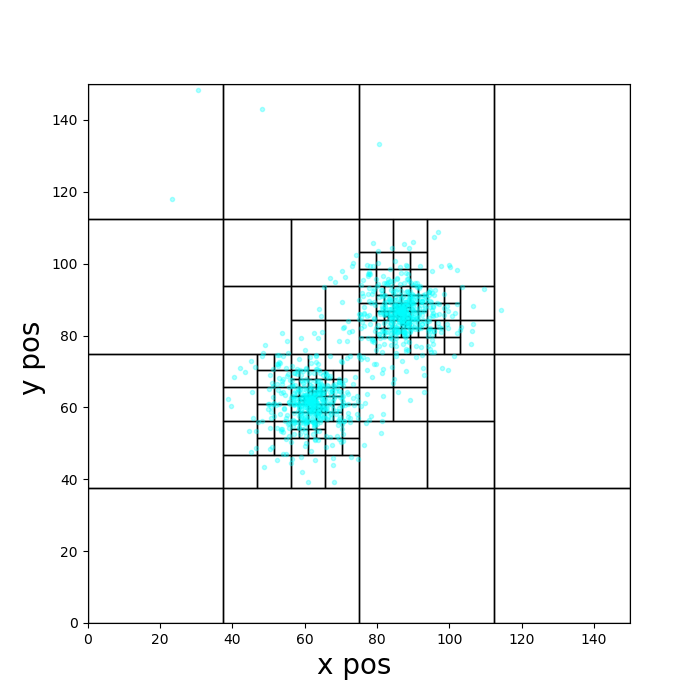
\includegraphics[width=0.9\linewidth]{./plots/quadtree.png}
    \caption{Quadtree plotted.}
    \label{quad}
\end{figure}


\section{Problem 8}
Not implemented. Sad!

Another small rant. I would like it to be known that Computational Astrophysics
is a course based entirely on simulations ($6$ ECs). There were $5$ assignments
that took several weeks to code up---\emph{with} the simulation backbone
already provided (via \texttt{AMUSE}). This problem could probably take a
month to complete on its own. And it is only worth a small fraction of the
final grade. I would love to continue talks on the expectations of this course
in the future.



\end{document}


\section{1}
\subsection{1a}

Here we test our rng as we did in the first handout. 
\begin{figure}[h!]
    \centering
    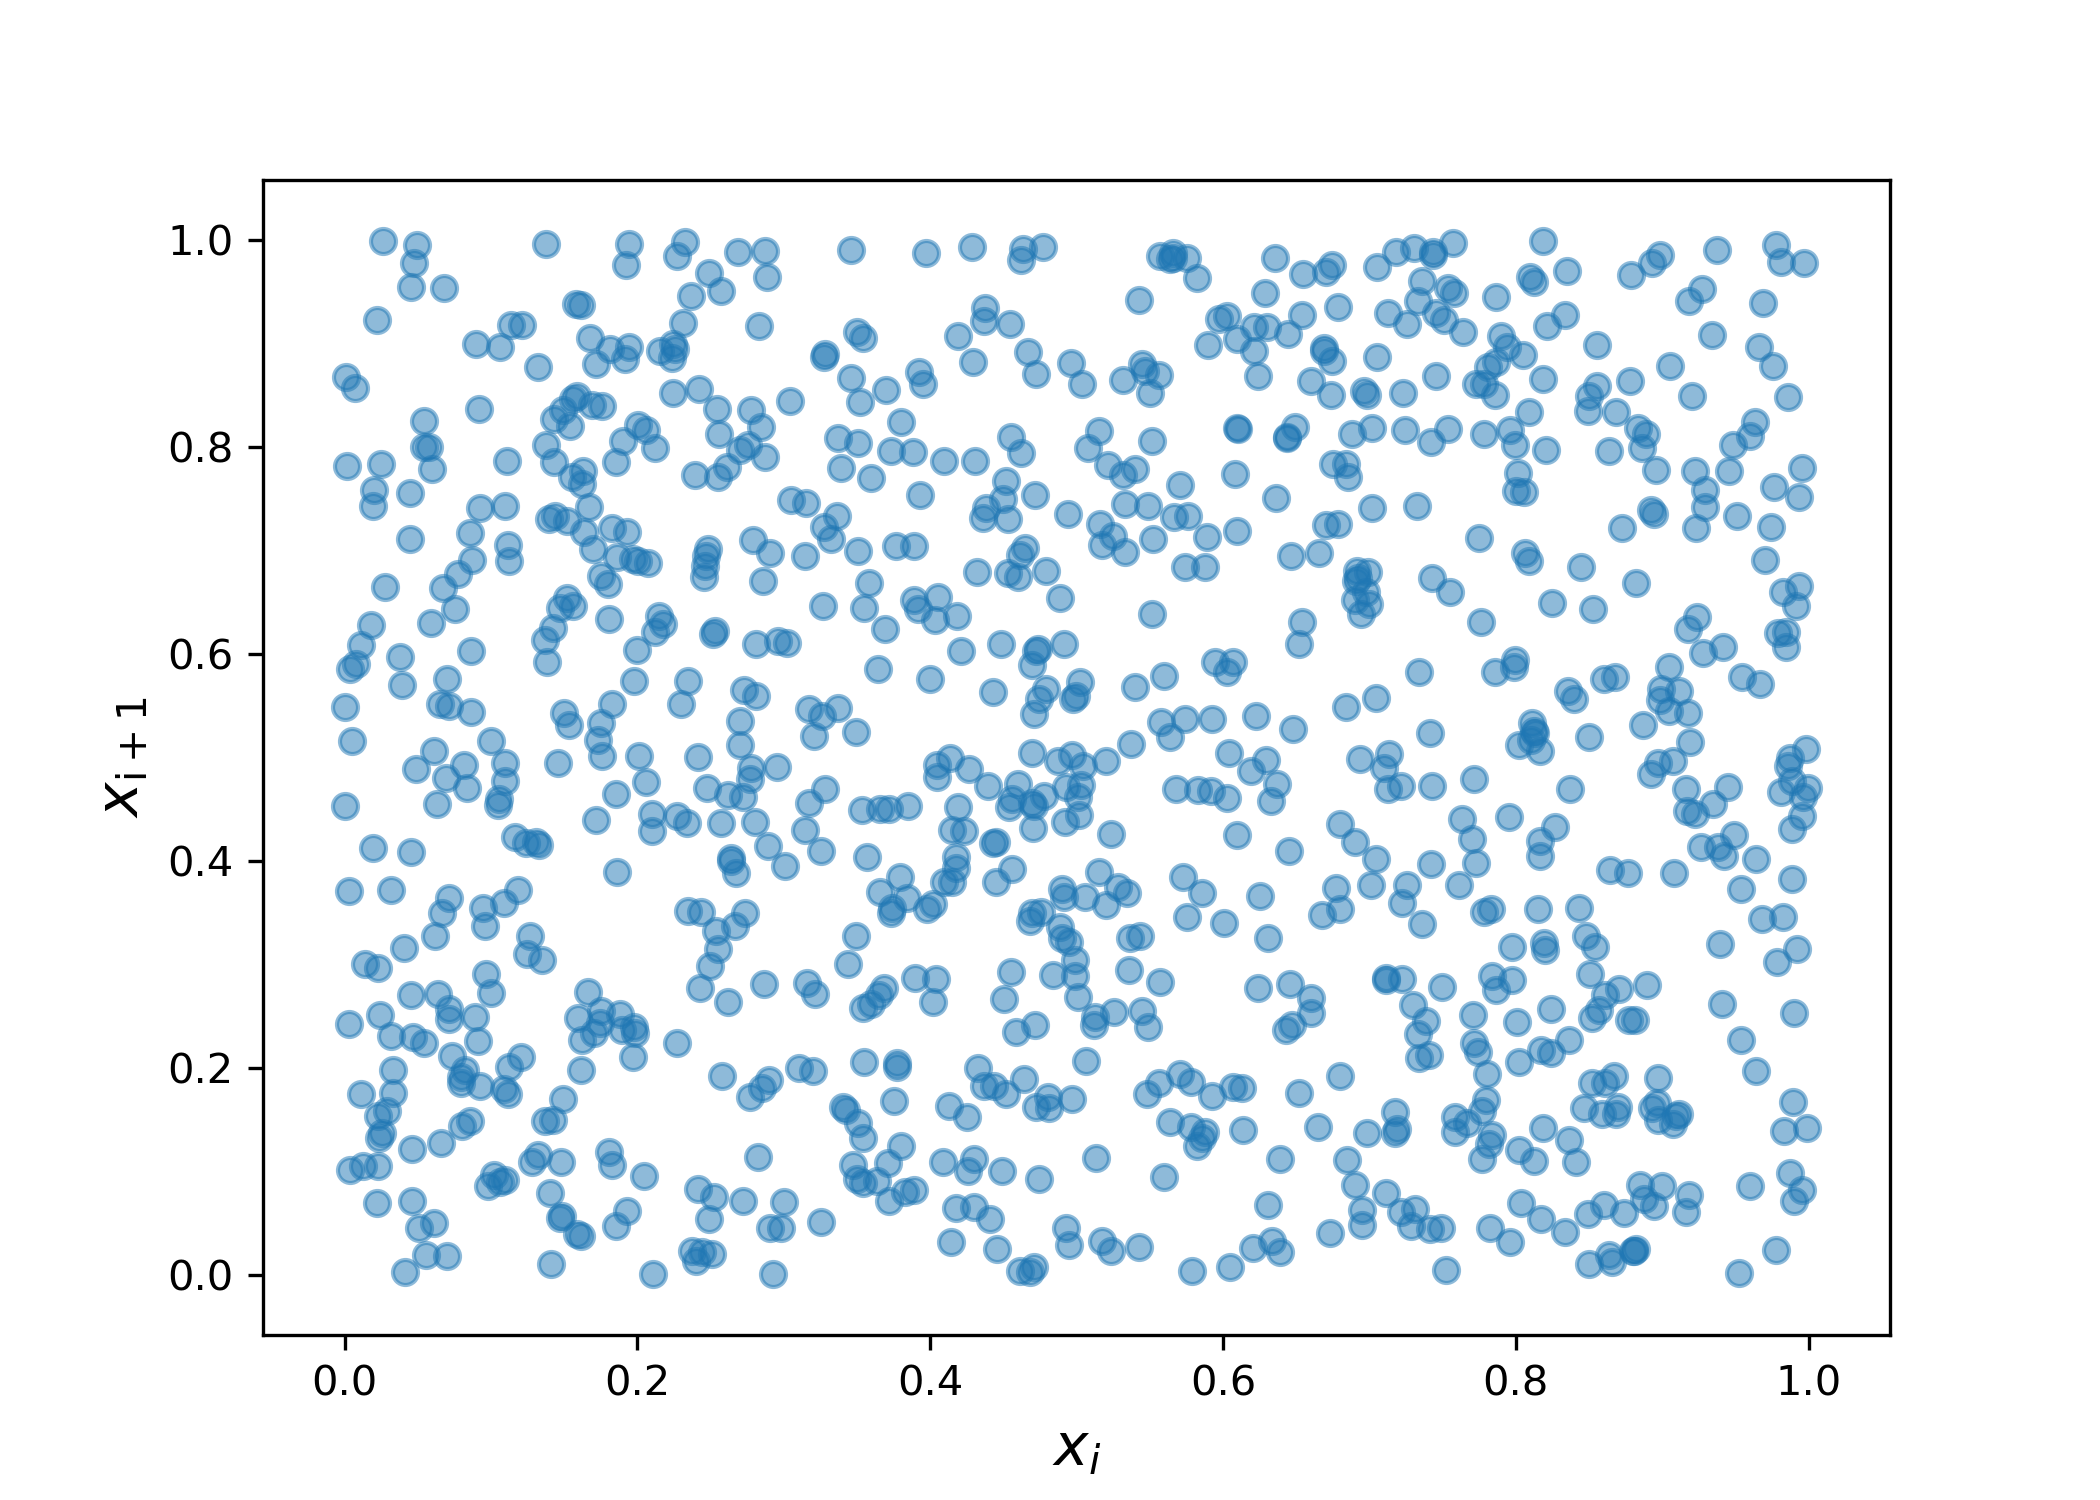
\includegraphics[width=0.9\linewidth]{./plots/x_x_1.png}
    \caption{$x$ vs. $x_{i+1}$ for the random number generator.}
    \label{plt1}
\end{figure}
Looking at the $i$ versus the $i+1$ components of our rng, there appears
to be little correlation between the numbers, which is a good sign. In
\autoref{plt2} we see the values that each number has in the array of 
$1000$ random numbers. It is between $0$ and $1$, also a good sign.
\begin{figure}[h!]
    \centering
    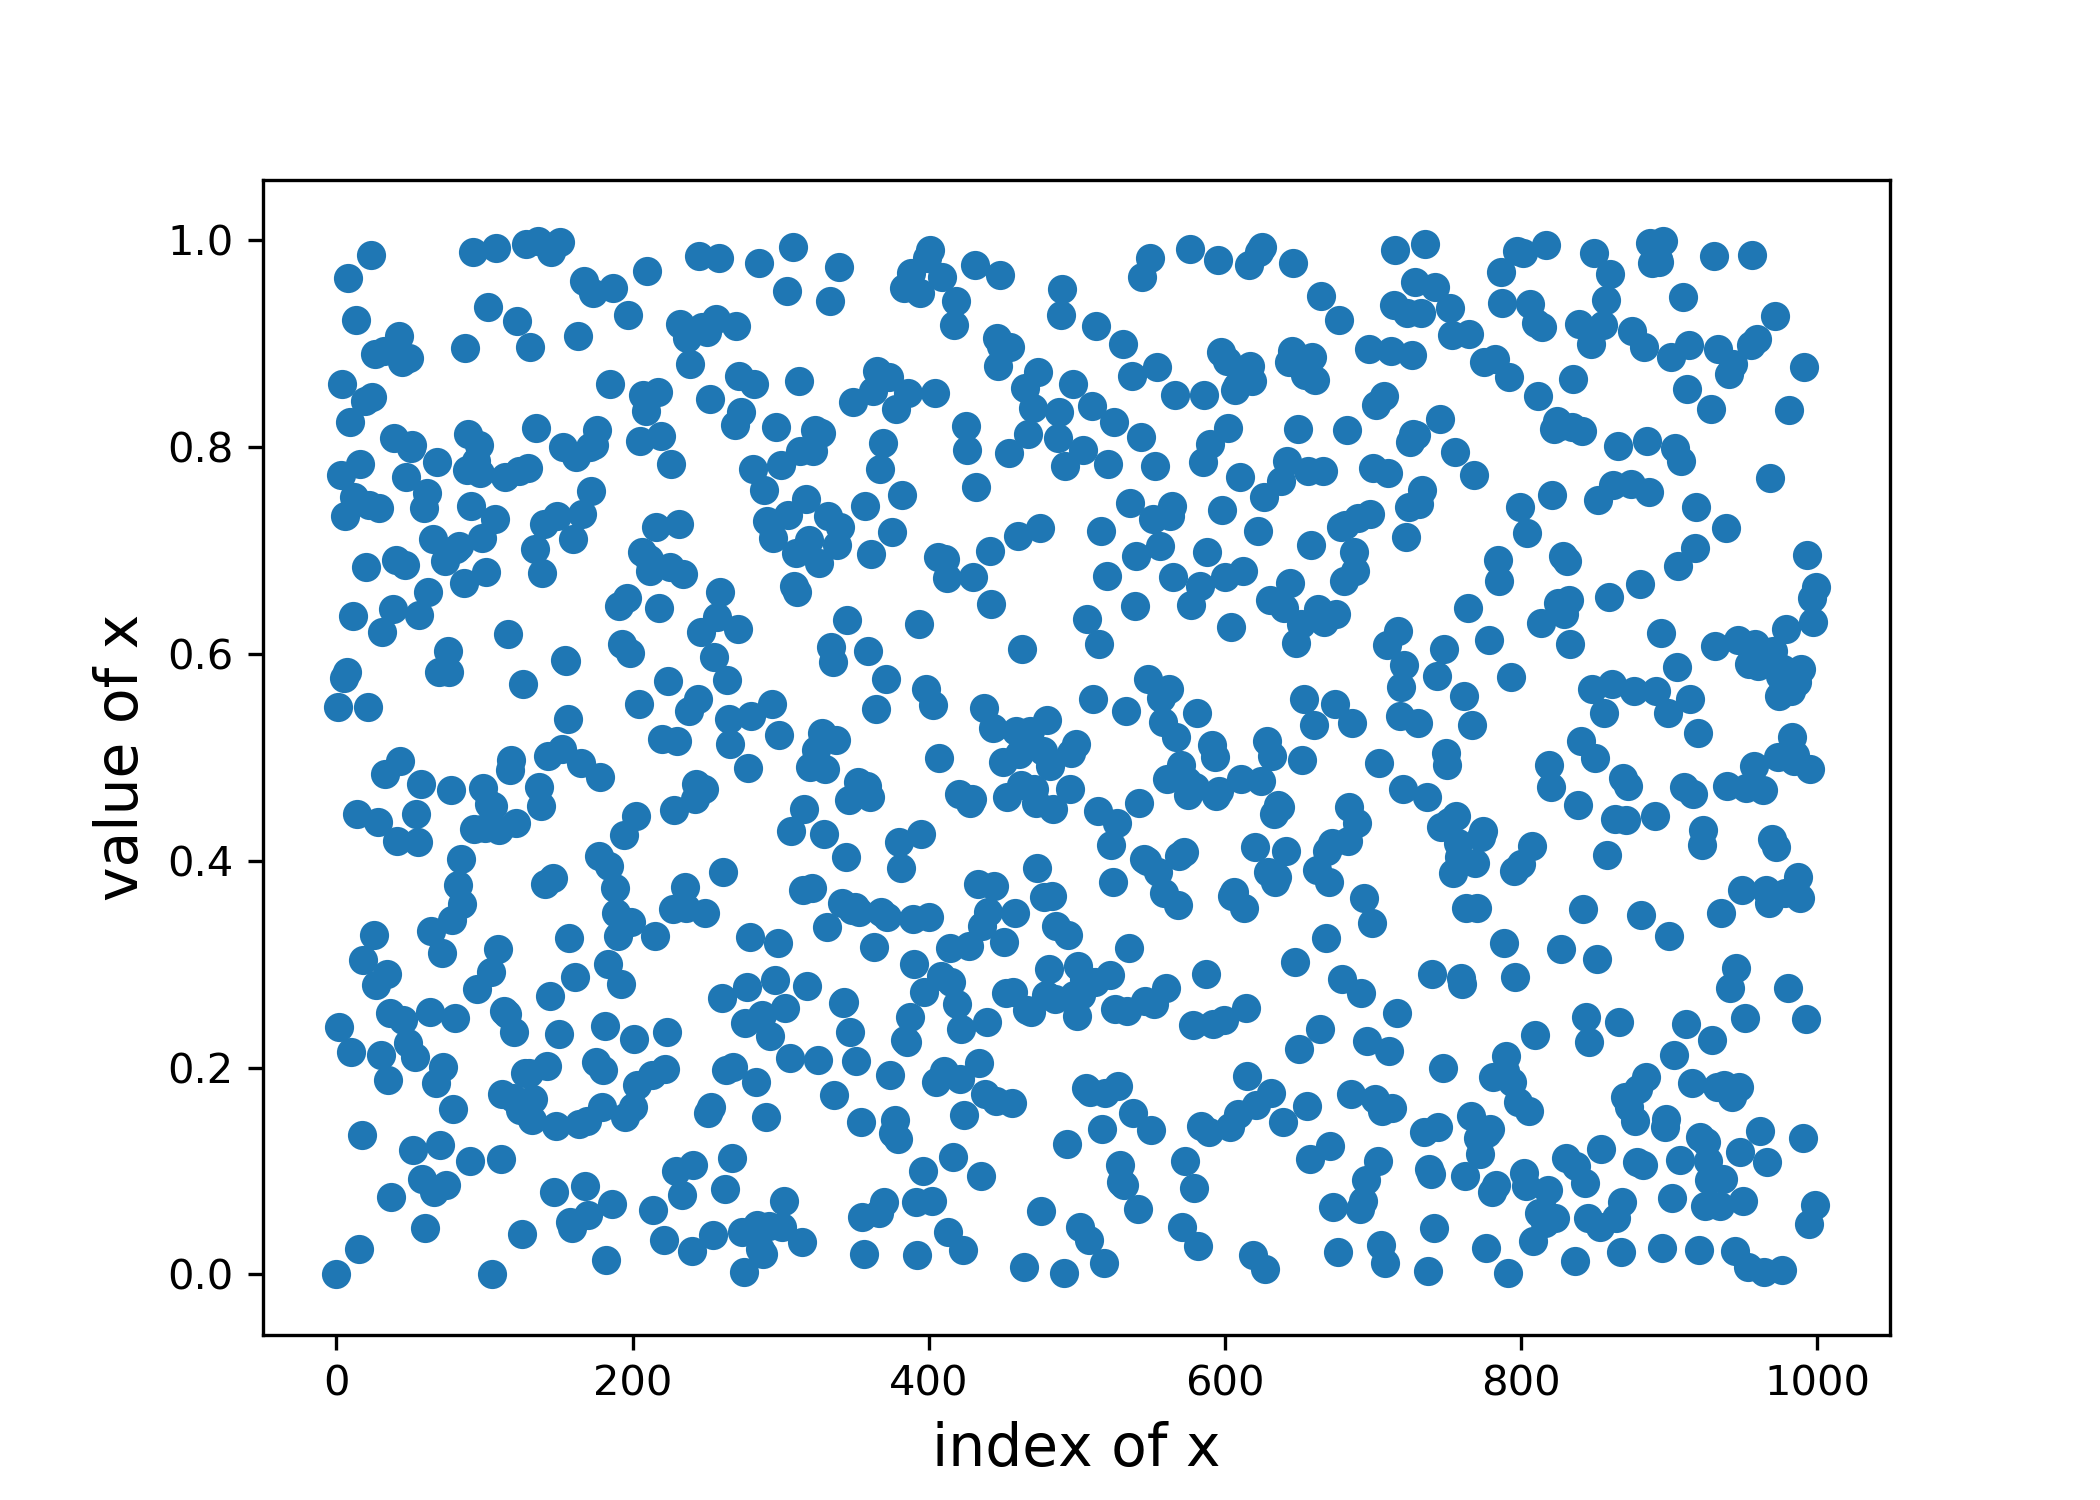
\includegraphics[width=0.9\linewidth]{./plots/xval_xind.png}
    \caption{The value of $x$ at a given index.}
    \label{plt2}
\end{figure}
However, in \autoref{plt3} it is clear something is wrong with the rng.
\begin{figure}[h!]
    \centering
    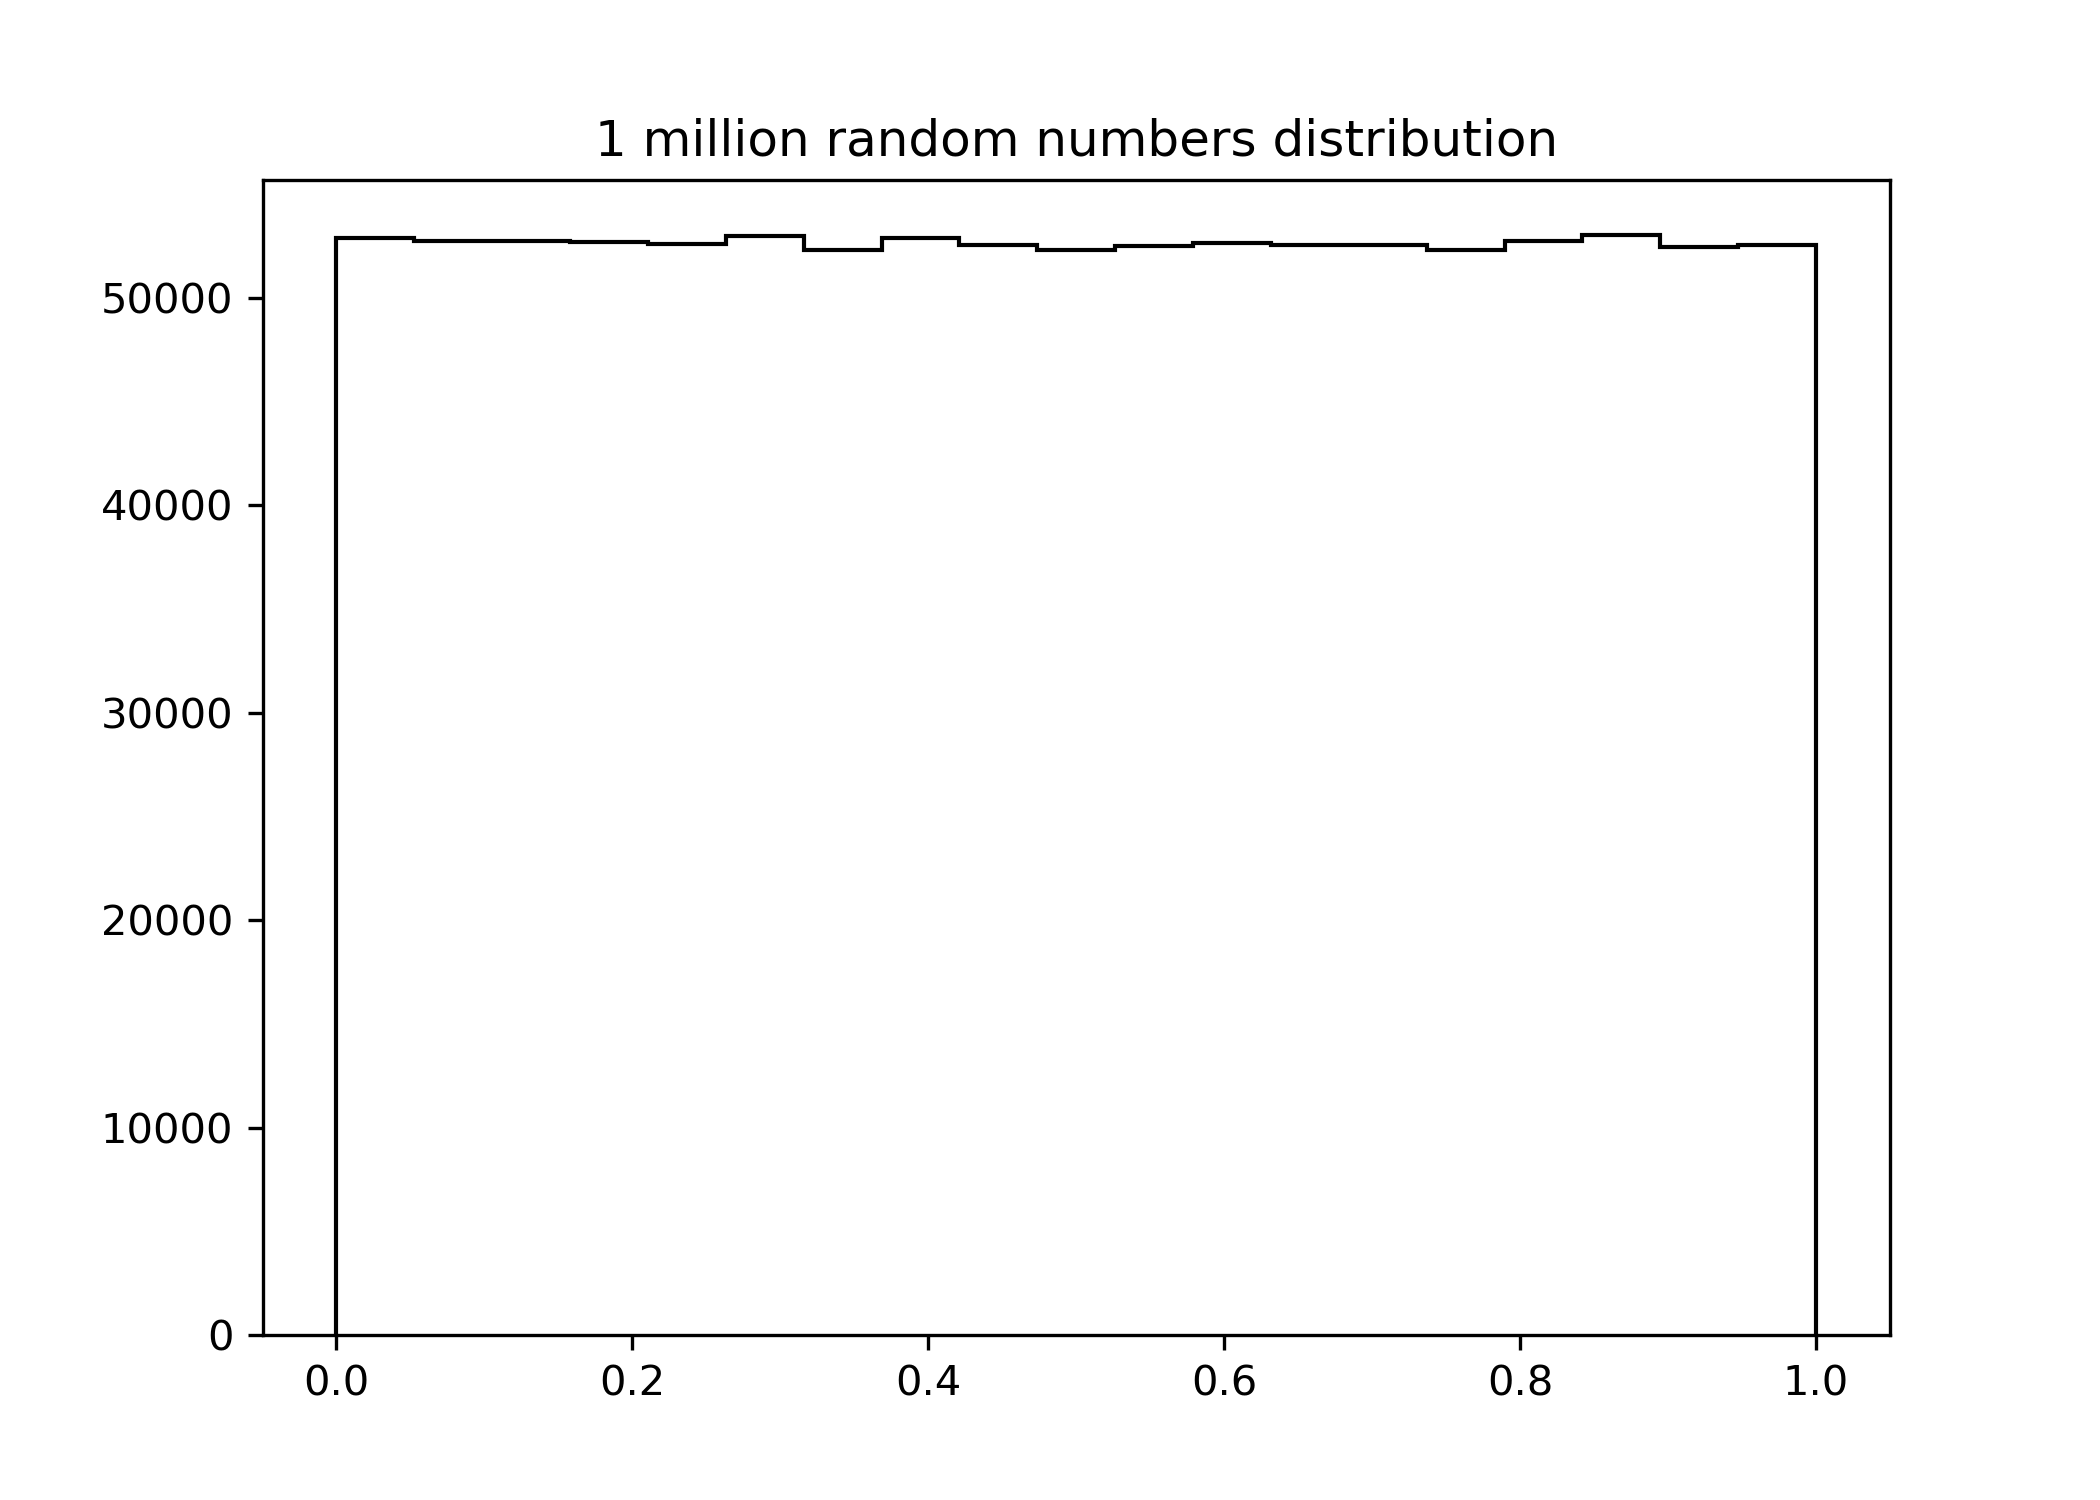
\includegraphics[width=0.9\linewidth]{./plots/1mil_hist.png}
    \caption{$1$ million random numbers plotted.}
    \label{plt3}
\end{figure}
As is plainly seen, the numbers in the random generator nearly all go above 
$5 \times 10^4$, which is not what we would expect from the rng. I am not
sure what the issue is. I attempted to cast all of the values as \texttt{ints}
but I was getting runtime errors in the $XOR$ bit-shift. The variance appears
to be fine, so I left it as is.


\subsection{1b}

\lstinputlisting{p1b.py}

As I have already explained that my rng is likely wrong, I will not mention
it further in the exercise. Here we use the Box-Muller method to generate
a Gaussian distribution, seen in \autoref{plt4}.
\begin{figure}[h!]
    \centering
    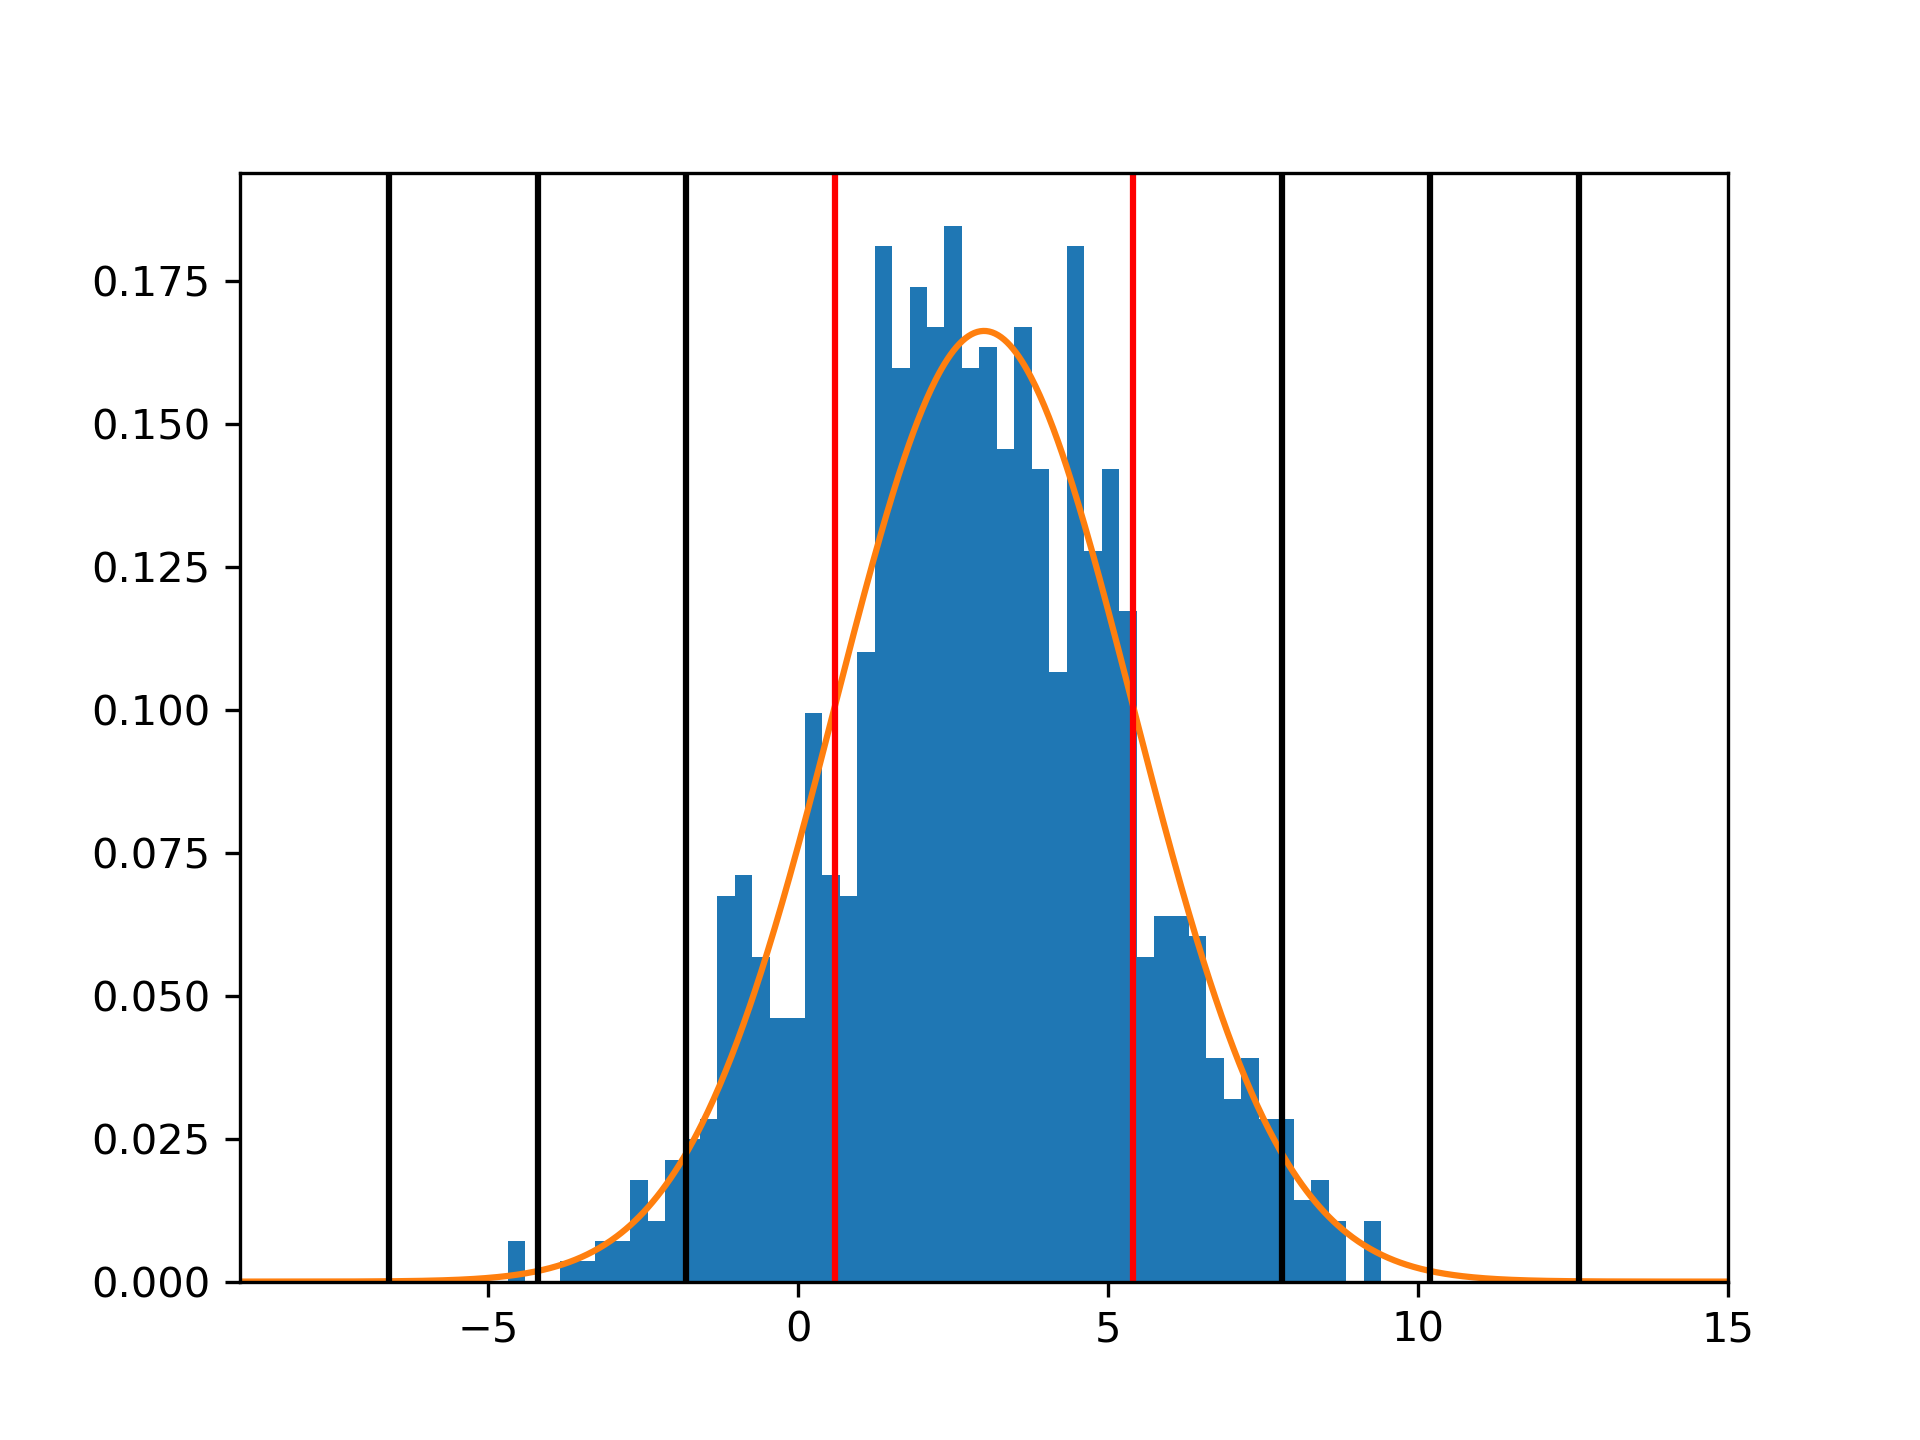
\includegraphics[width=0.9\linewidth]{./plots/box_gauss.png}
    \caption{My distribution with \texttt{numpy.norm} overplotted.}
    \label{plt4}
\end{figure}
The Box-Mueller method seems to work nicely, it is simply the rng that
ruins the Gaussian, given that there are values that are favored in the
$+1\sigma$ range.


\subsection{1c}

\lstinputlisting{p1c.py}
Next is the KS test. For this, I am unsure where I went wrong because
I followed the slides but to no avail. With time constraints, I was not
able to figure it out. Figures are plotted below.
\begin{figure}[h!]
    \centering
    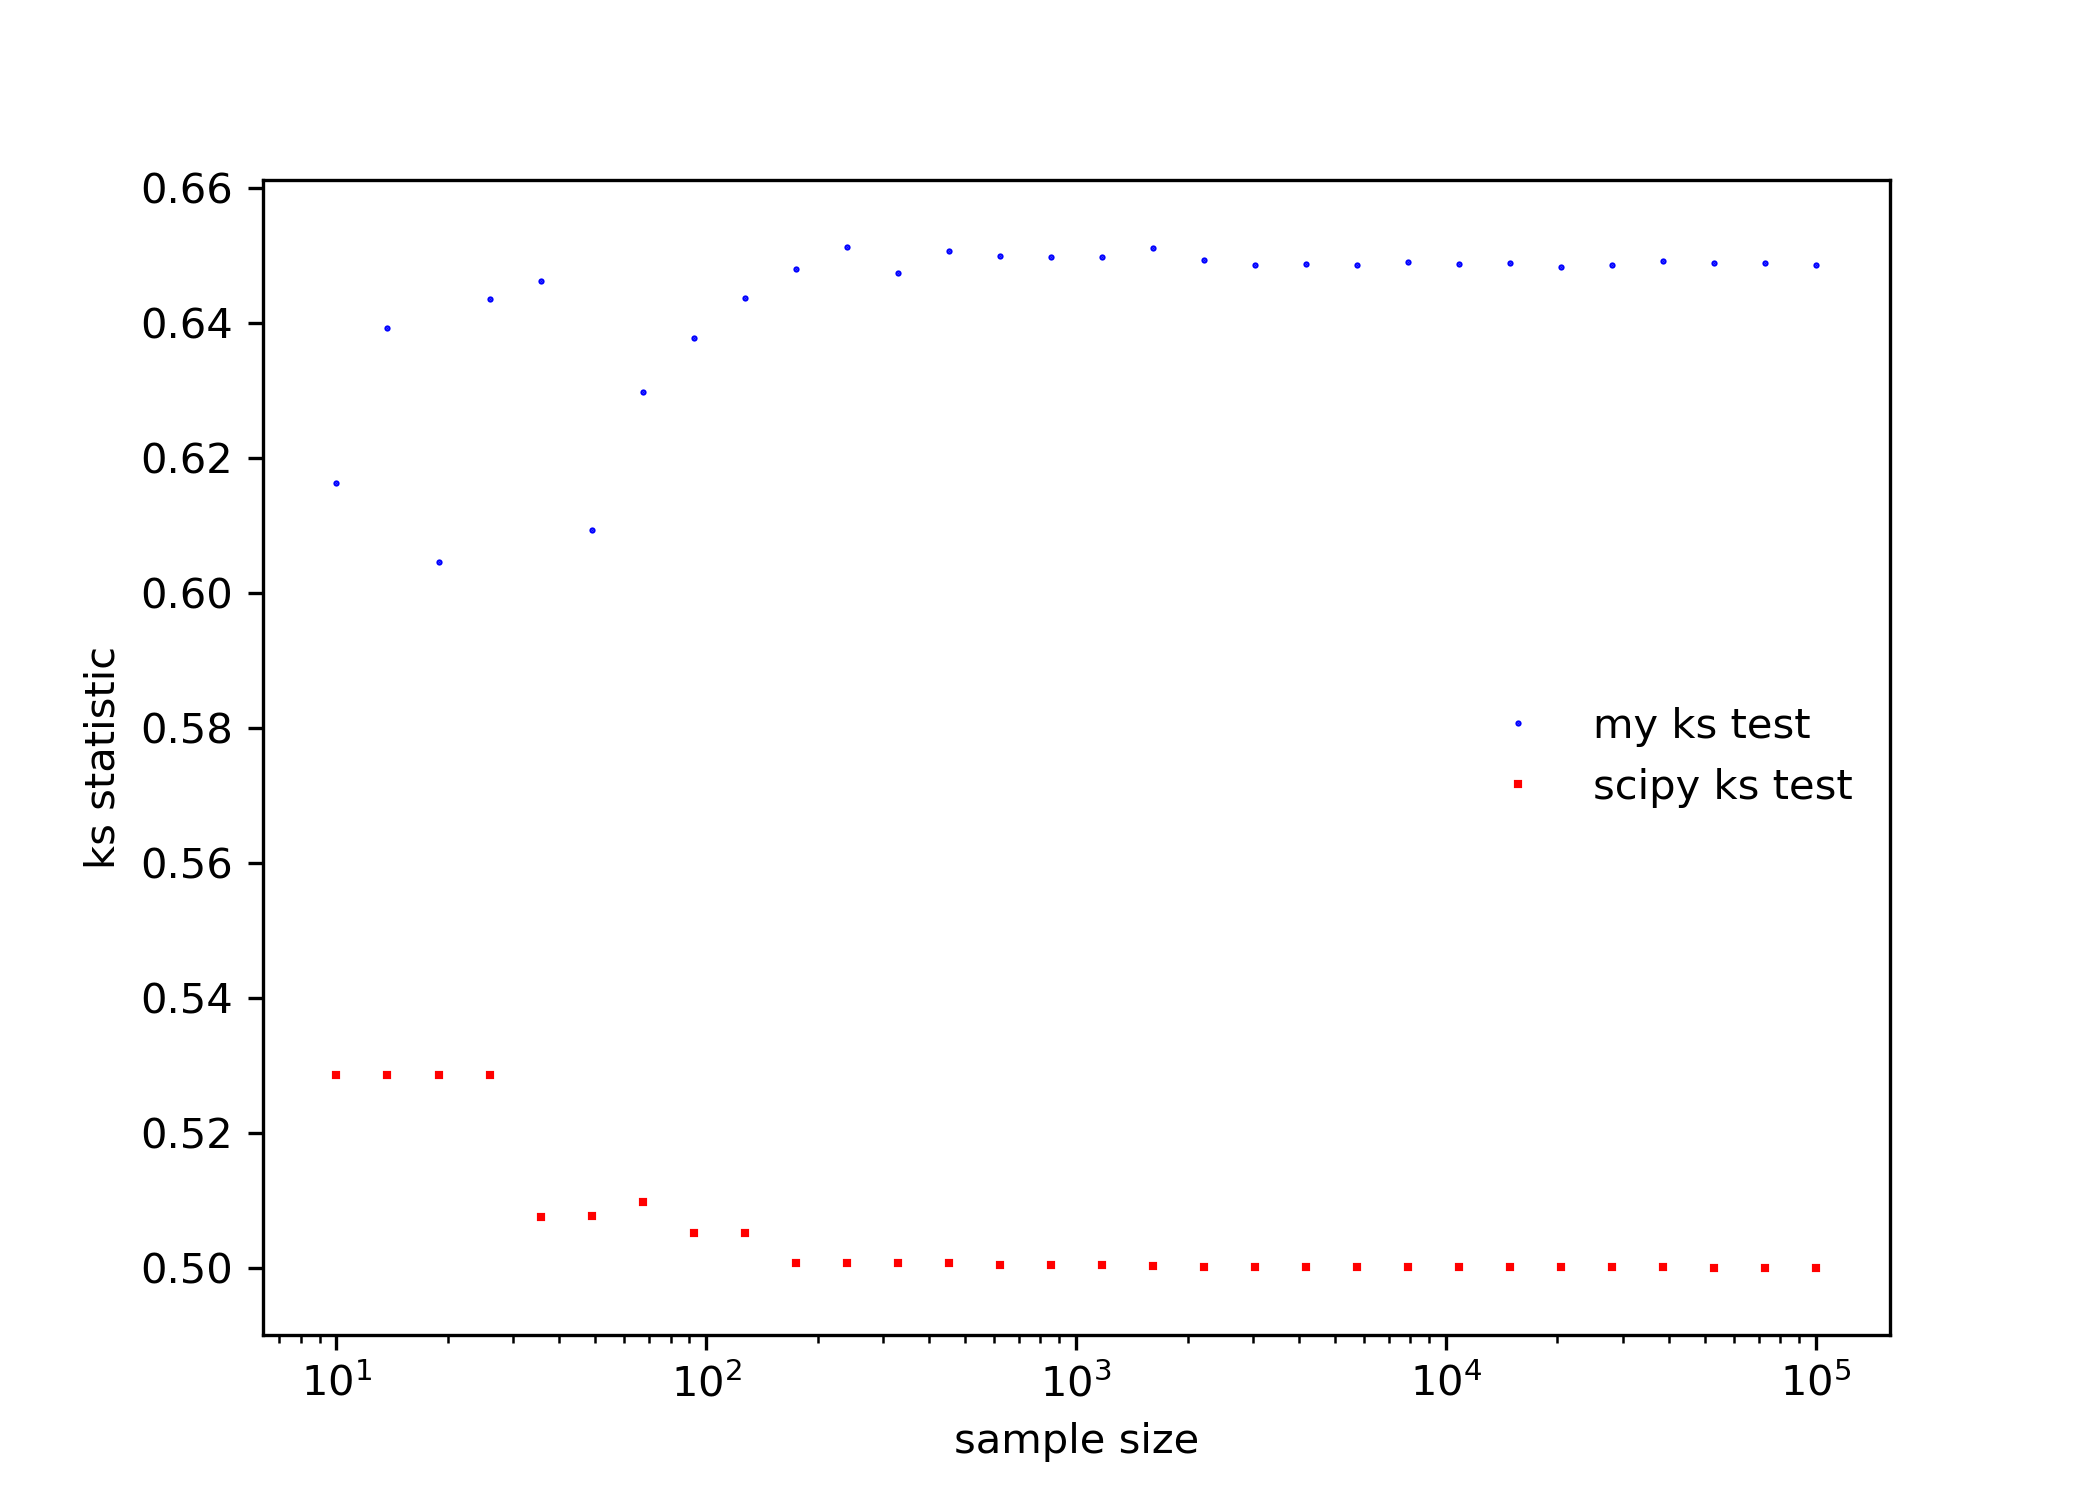
\includegraphics[width=0.9\linewidth]{./plots/ks_stat.png}
    \caption{$1$ million random numbers plotted.}
    \label{plt3}
\end{figure}

\begin{figure}[h!]
    \centering
    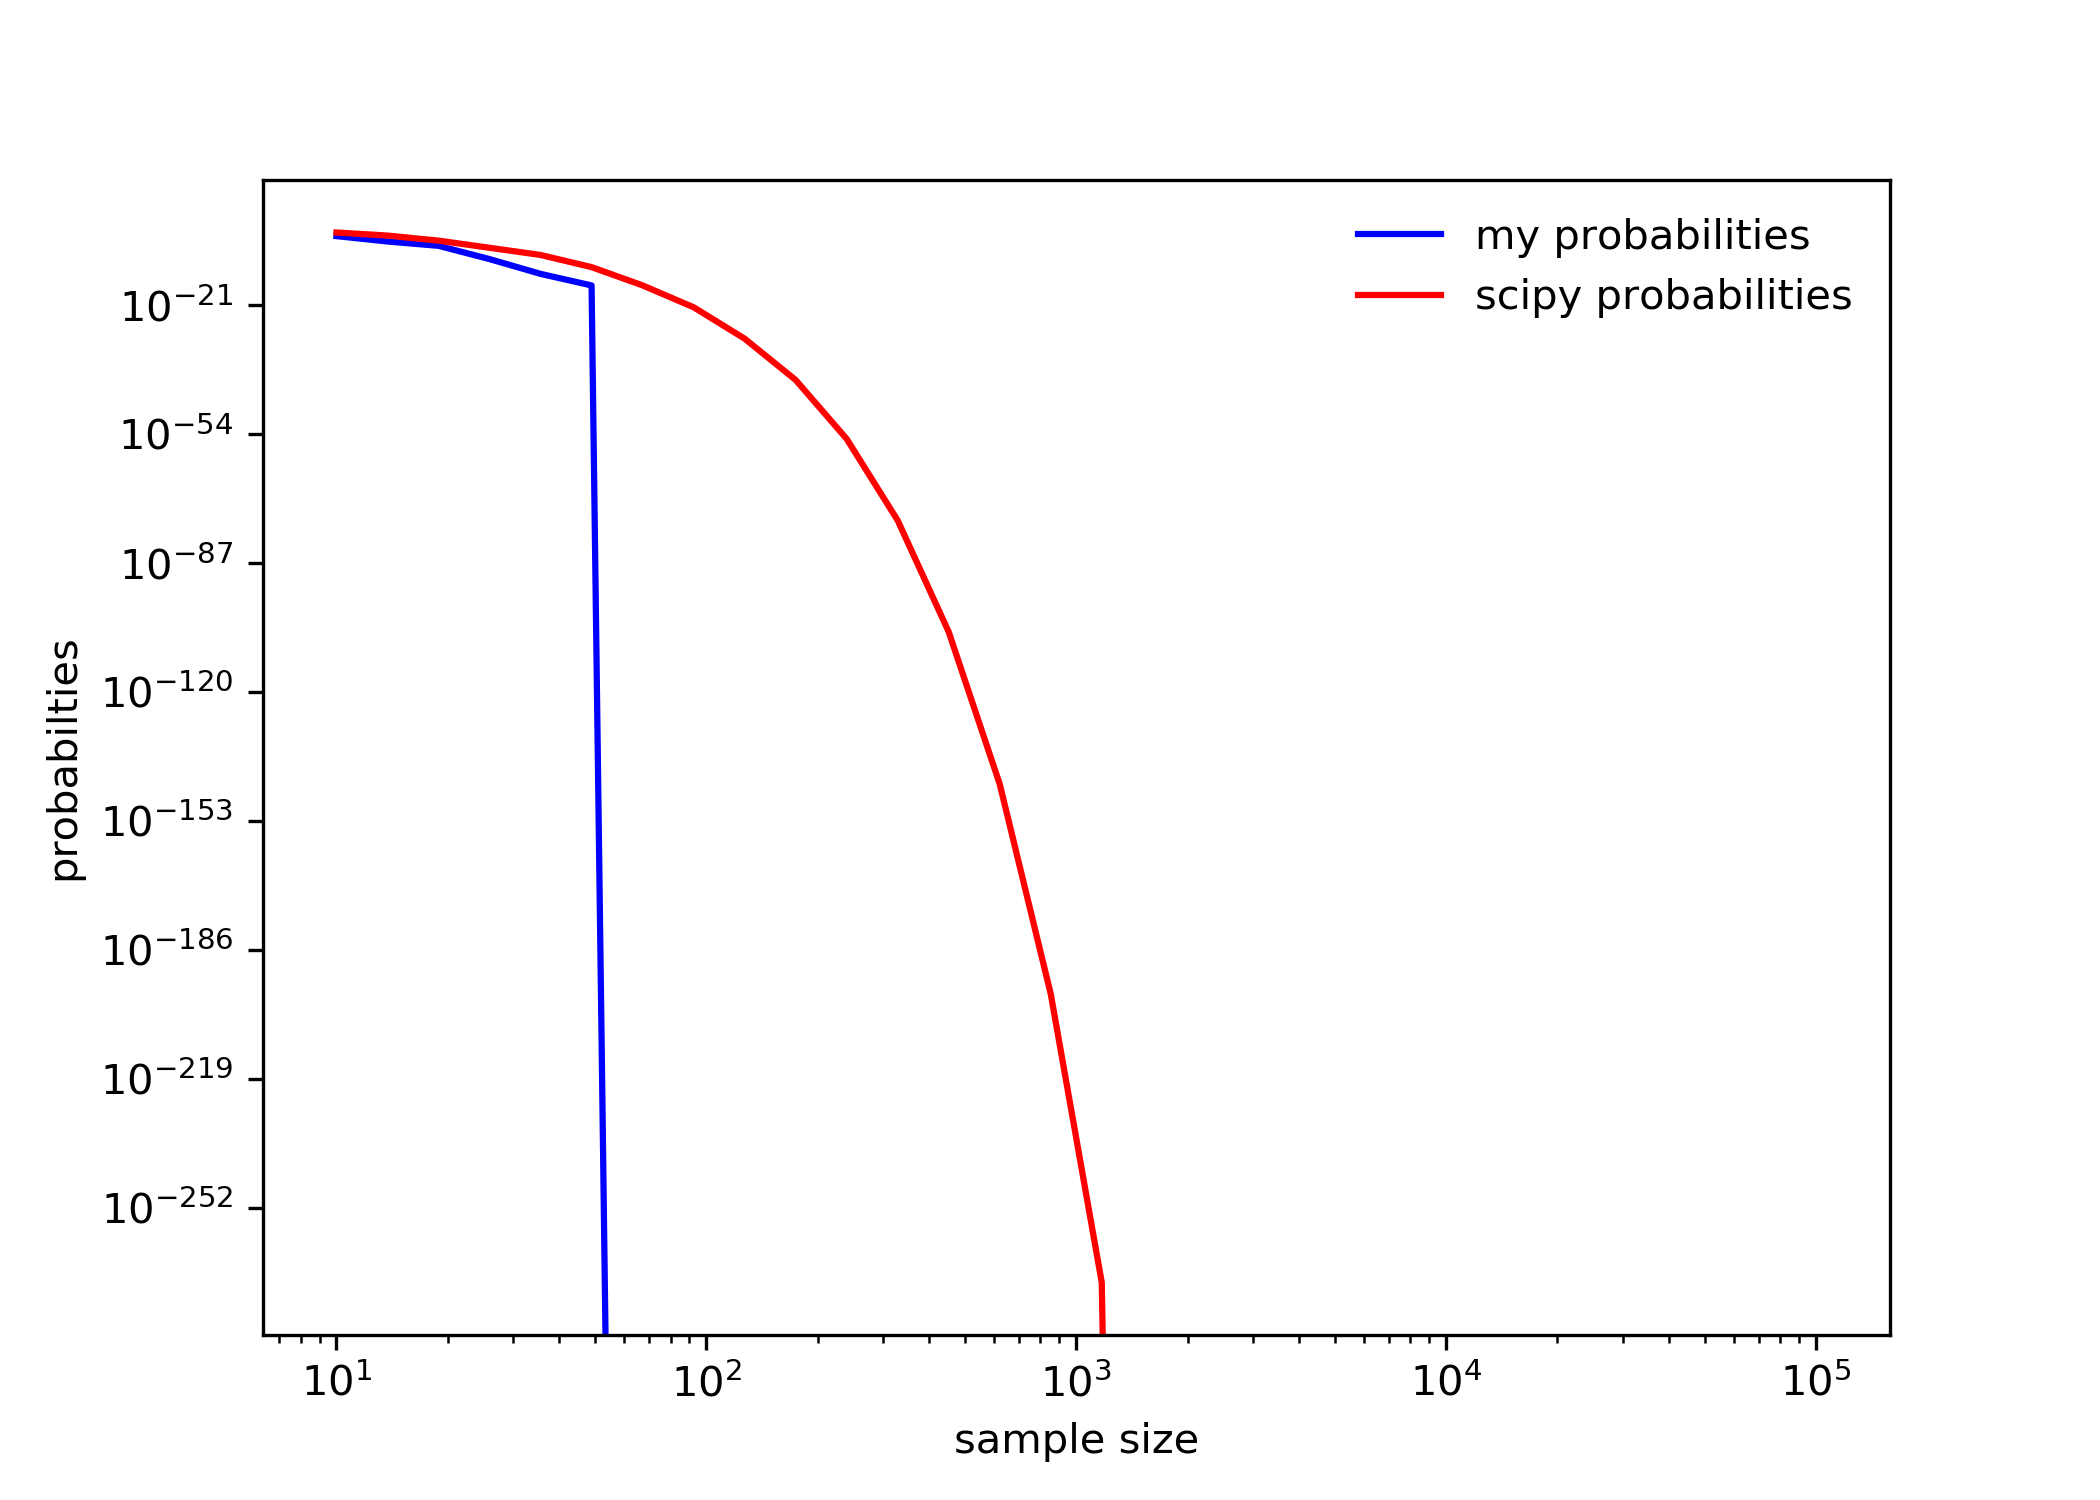
\includegraphics[width=0.9\linewidth]{./plots/ks_prob.png}
    \caption{$1$ million random numbers plotted.}
    \label{plt3}
\end{figure}



\subsection{1d}

\lstinputlisting{p1d.py}
Next is the Kuiper test. As with the KS test, I am unsure where I went wrong
because I followed the slides but to no avail. With time constraints, 
I was not able to figure it out. Figures are plotted below. One obvious 
explanation is that my distribution does not fit a Gaussian.
I am unsure of potential (and likely) bugs in my code.
\begin{figure}[h!]
    \centering
    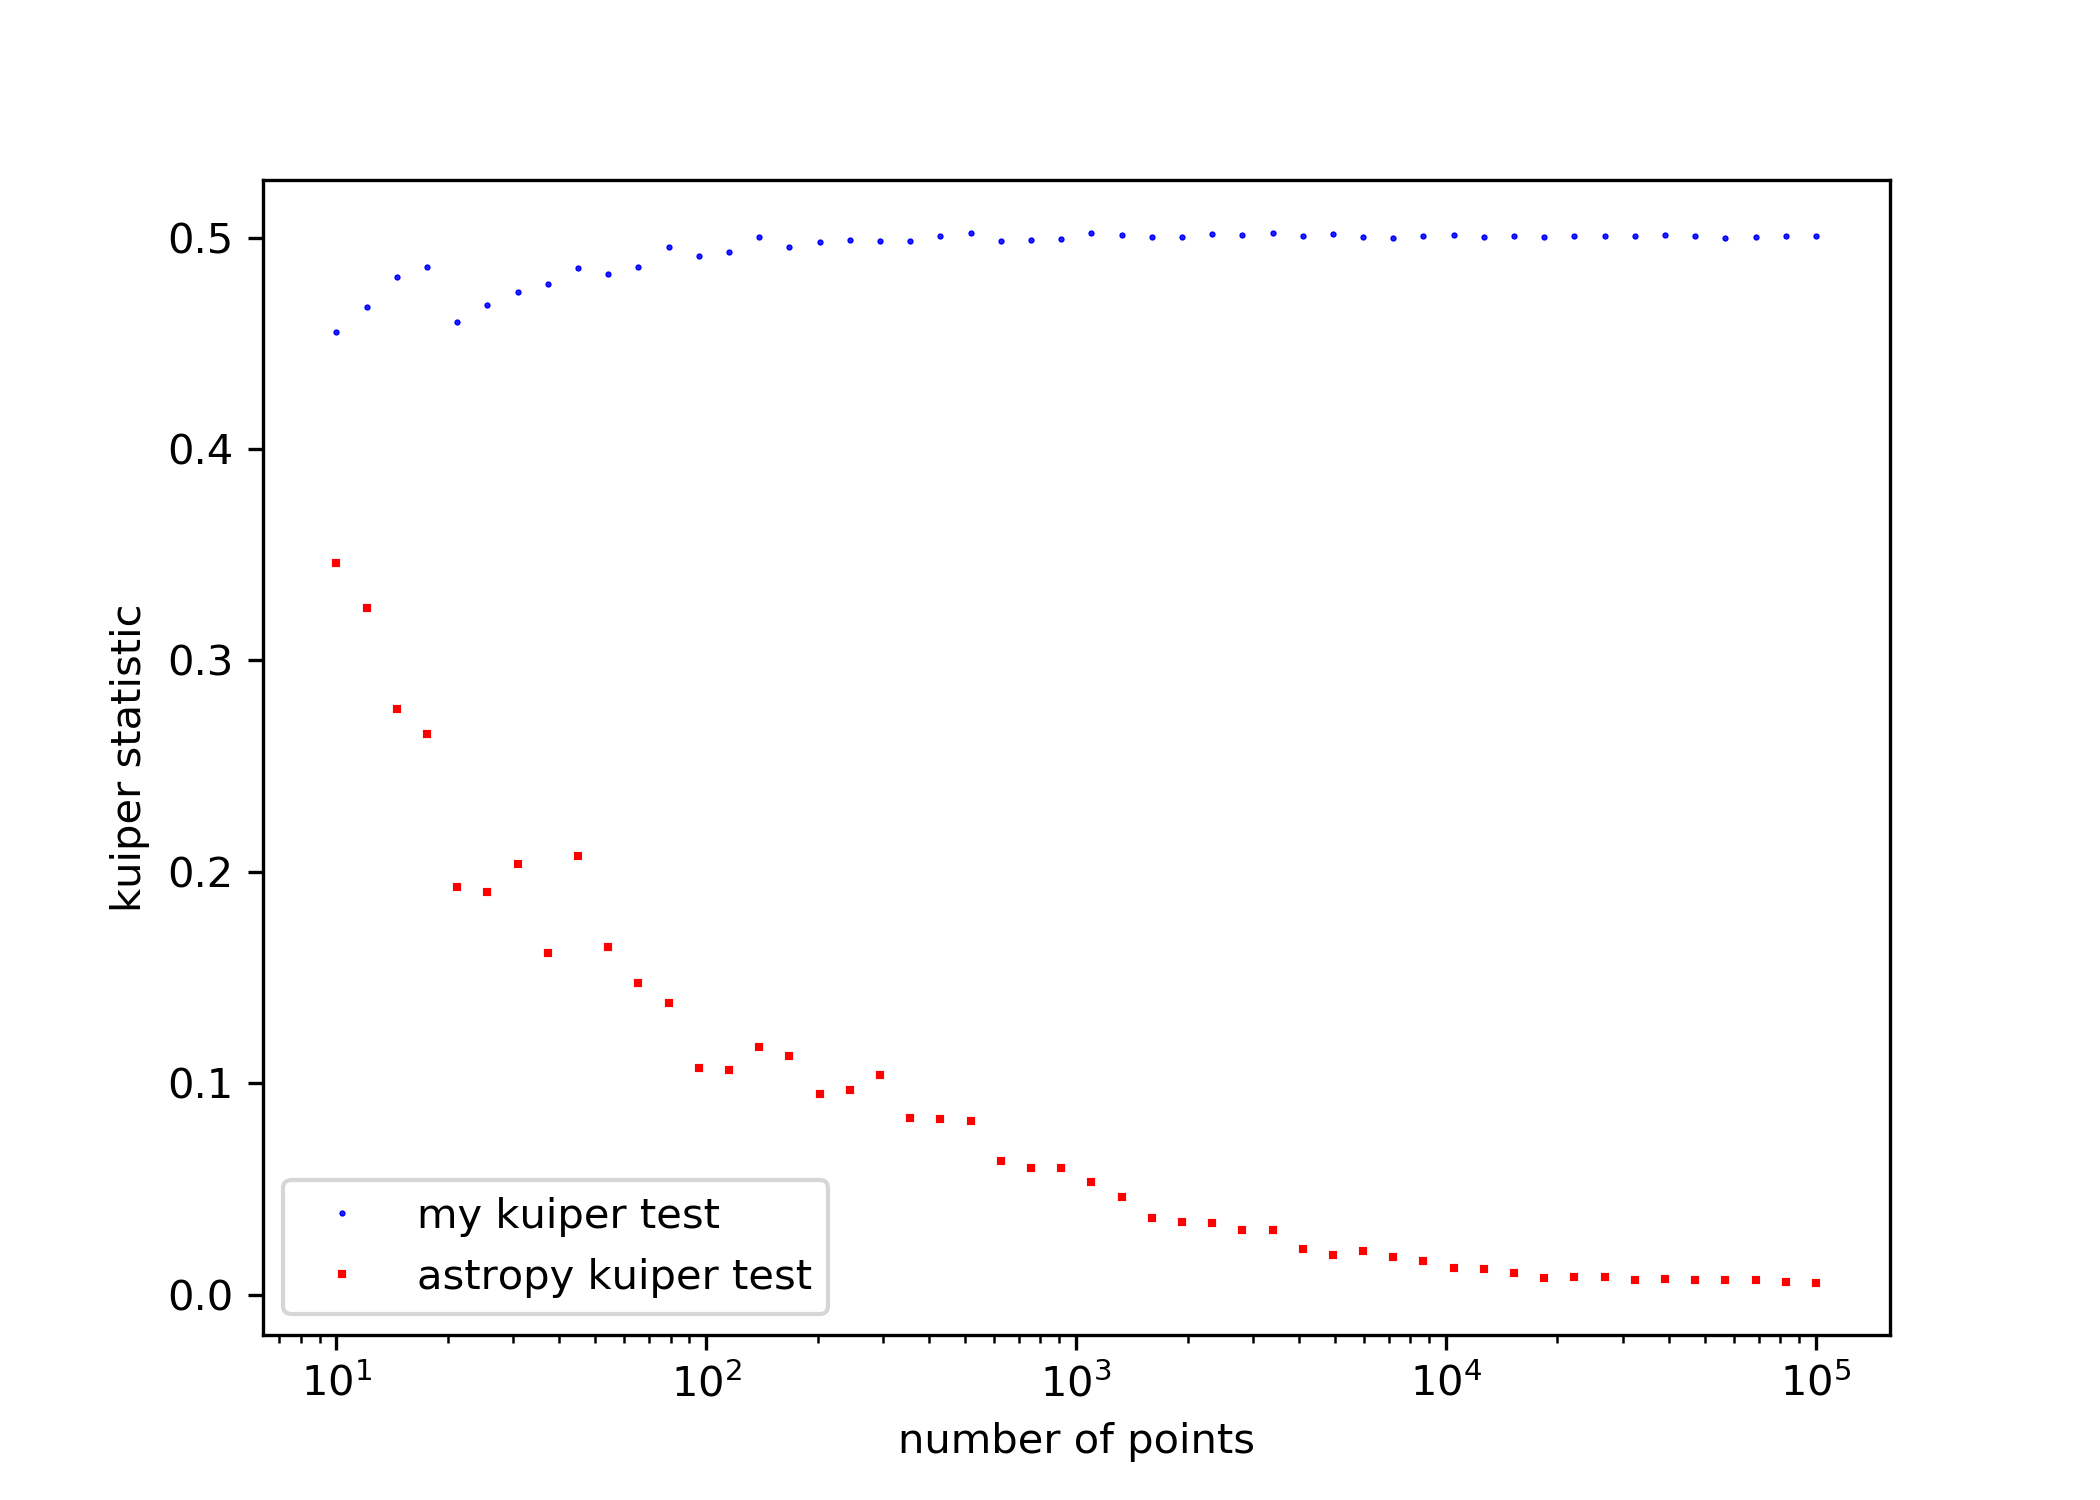
\includegraphics[width=0.9\linewidth]{./plots/kuiper_stat.png}
    \caption{Kuiper distance statistic.}
    \label{kuip_s}
\end{figure}

\begin{figure}[h!]
    \centering
    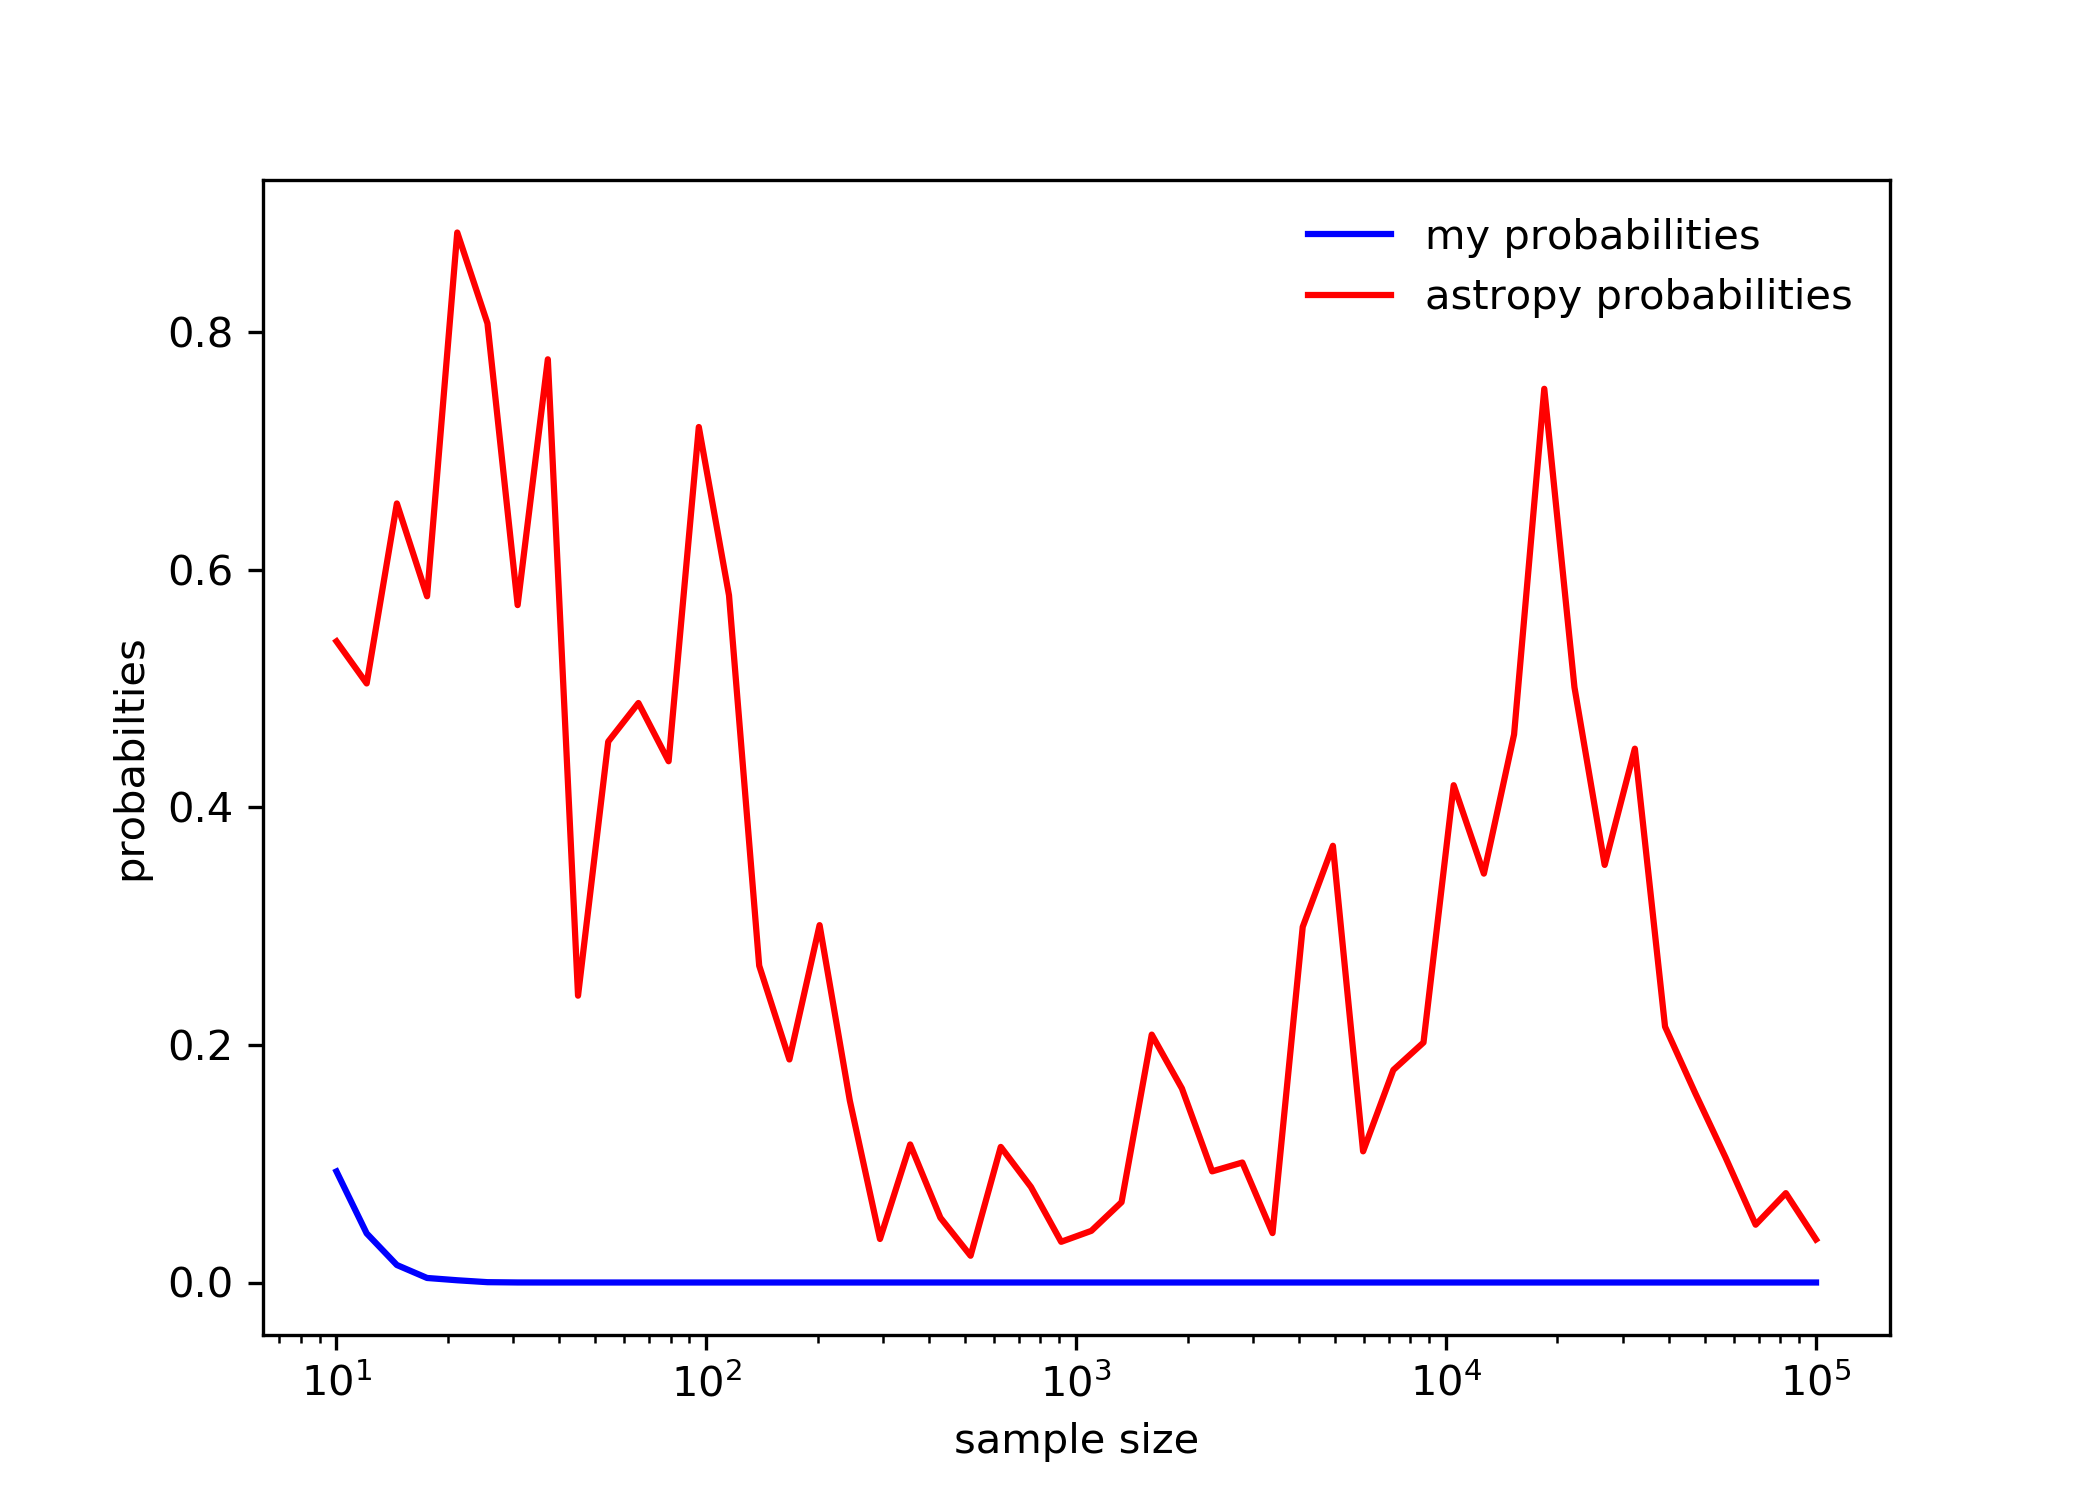
\includegraphics[width=0.9\linewidth]{./plots/k_prob.png}
    \caption{Kuiper probabilities.}
    \label{kuip_p}
\end{figure}



\subsection{1e}

\lstinputlisting{p1e.py}
Next, we are meant to verify a statistic of our choice (in this case the 
KS statistic) with a set of random numbers. I recognized too late that I need
to implement a $2$D KS sampler. As can be seen, I have a potential CDF to use,
but the statistic cannot be used at this time.



\section{Problem 2}

\lstinputlisting{p2.py}
We set out to make initial density fields based off of the power spectrum,
\begin{equation}
  P(k) = k^n,
\end{equation}
where $n$ is $-1, -2, -3$. Essentially, we setup the indices for the Fast
Fourier Transform (FFT) as described in the slides. We define the function
for the power spectrum, use our rng to make random numbers, and finally
perform the FFT on each field. Figures are plotted below.

\begin{figure}[h!]
    \centering
    \includegraphics[width=0.9\linewidth]{./plots/gauss_field_n_1.png}
    \caption{Gaussian field for $n=-1$.}
    \label{gf1}
\end{figure}
The initial field in \autoref{gf1} looks roughly what we expect.
Admittedly, I am unsure exactly what is expected, but as the handout
explains, dispersion is dependent on $n$. In \autoref{gf2} we can see
the dispersion causes a bit more ``clumpiness'' (that is, high-density
pockets). In \autoref{gf3}, we see an even higher contrast between
the low-high density regions. (Sorry, my colorbar was not working! It's 
viridis colormap, though.)
\begin{figure}[h!]
    \centering
    \includegraphics[width=0.9\linewidth]{./plots/gauss_field_n_2.png}
    \caption{Gaussian field for $n=-2$.}
    \label{gf2}
\end{figure}
However, in \autoref{gf3} it is clear something is wrong. The physical
distances are not changing as a function of $n$. As $P_k$ changes from
$n=-1$ to $n=-2$ for example, the maximum and minimum k values should increase
from $n=-1$ to $n=-2$. The physical distances should be larger as well.
Given time constraints, I gave up and left the plots as is. I assume 
it has a $2$-fold issue: my rng and perhaps the amplitudes are not actually
changing as expected.
\begin{figure}[h!]
    \centering
    \includegraphics[width=0.9\linewidth]{./plots/gauss_field_n_3.png}
    \caption{Gaussian field for $n=-3$.}
    \label{gf3}
\end{figure}



\section{Problem 3}

\lstinputlisting{p3.py}
We set out to solve the given ordinary differential equation (ODE) given in
the handout. I have very little to show--I do not have the analytic solution,
and it is clear from \autoref{rk} that the solution is not correct. My attempt
was to decompose the second-order ODE to a first-order, then to use the
Runge-Kutta fourth-order algorithm to solve the ODE. Results are below.
I needed much more help than I sought out, I recognize that. But, it was also
important to try and do the rest of the assignment as well...

\begin{figure}[h!]
    \centering
    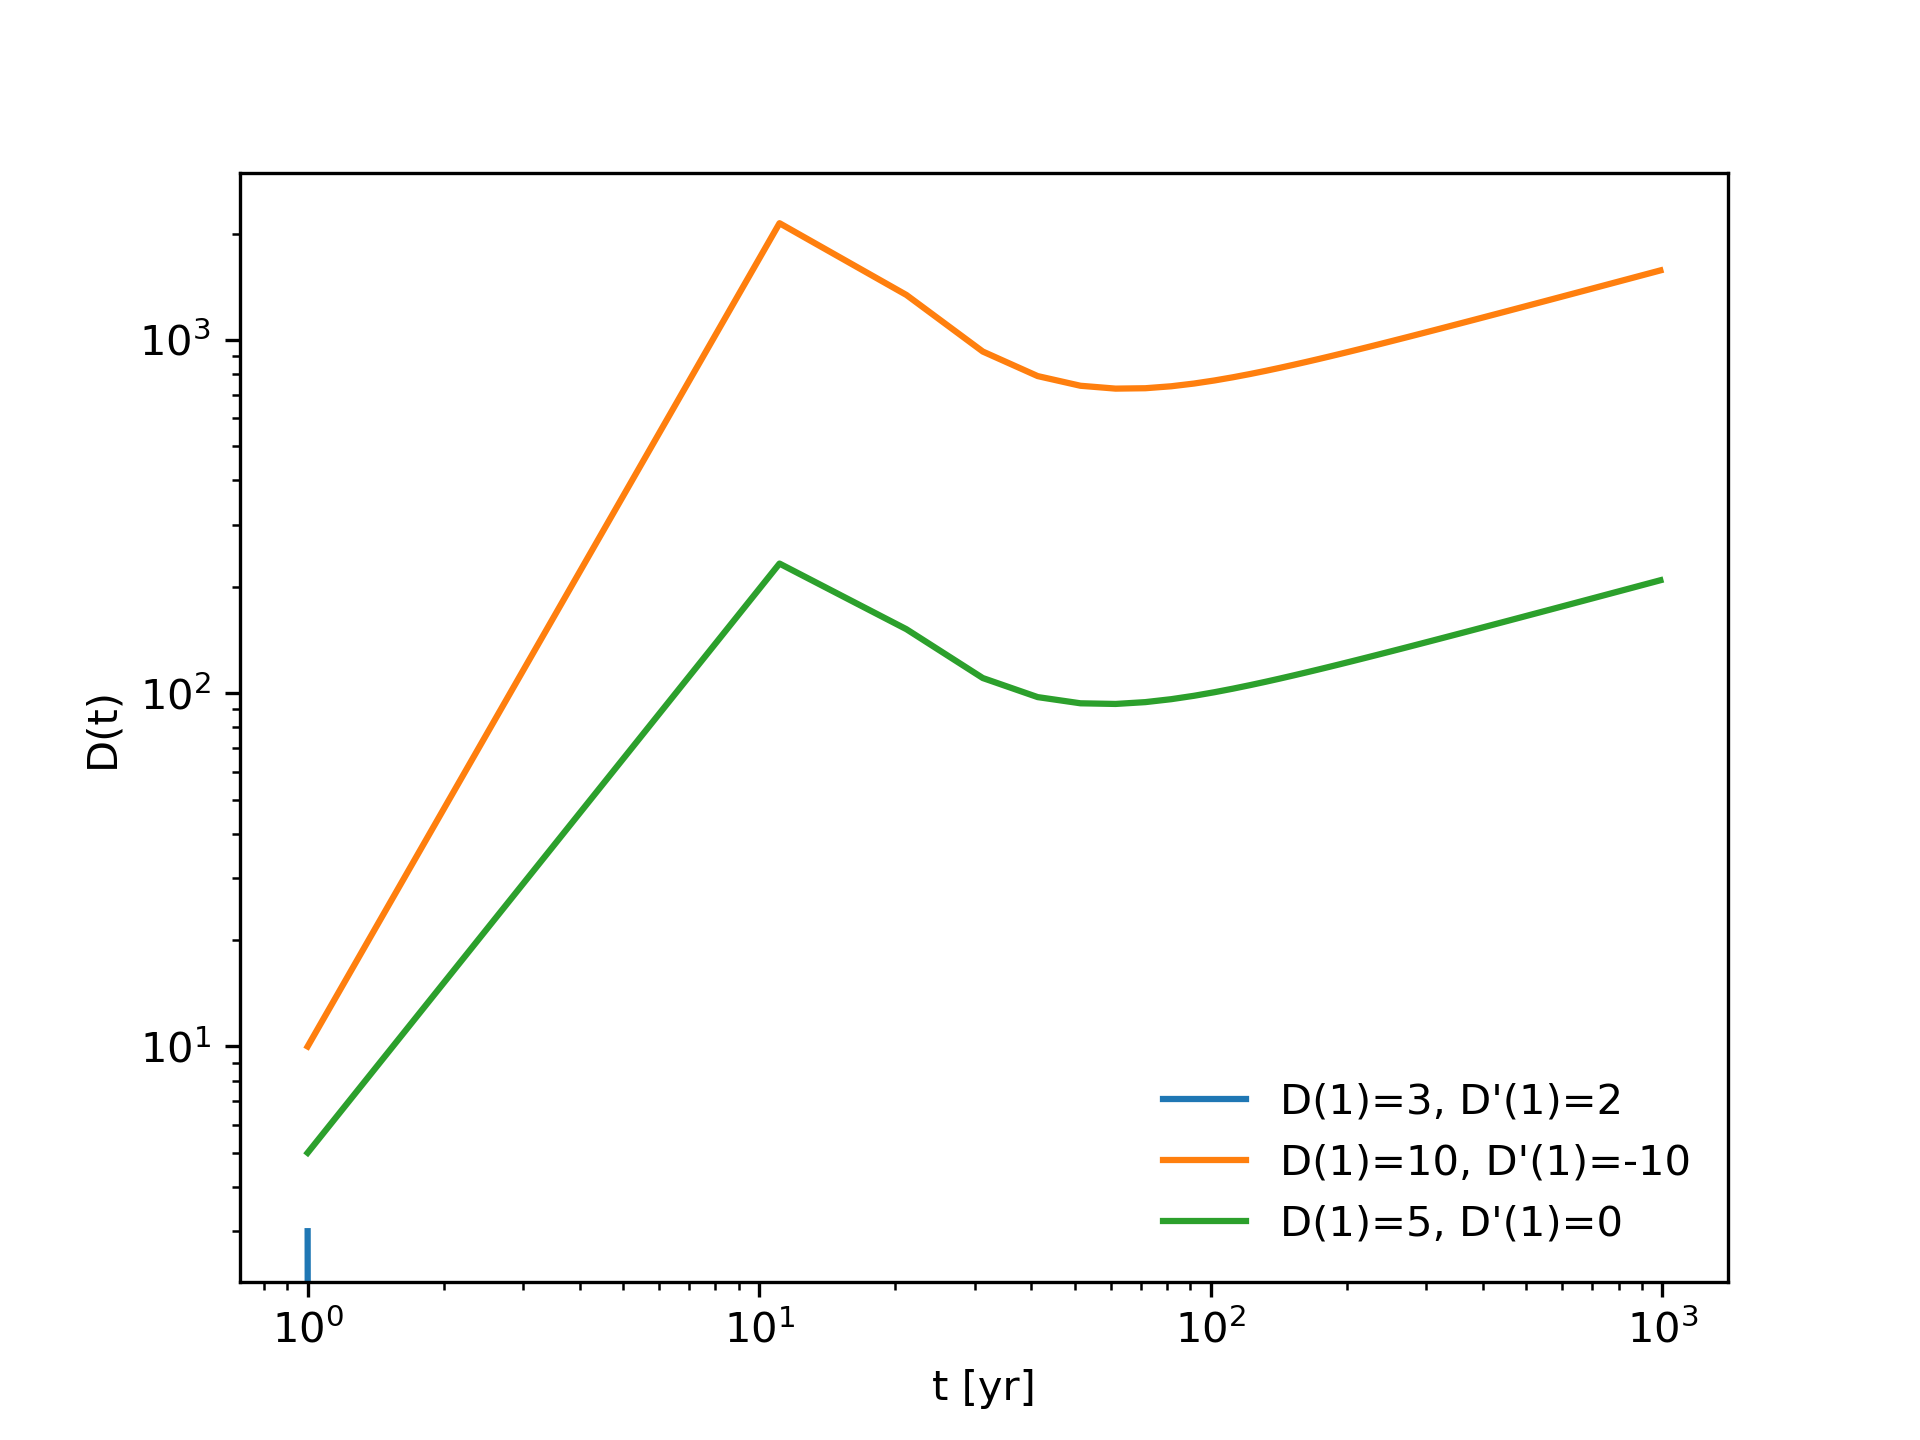
\includegraphics[width=0.9\linewidth]{./plots/rk4.png}
    \caption{Sad plot of the ODE solved.}
    \label{rk}
\end{figure}



\section{Problem 4}
\subsection{4a}

\lstinputlisting{p4a.py}
\lstinputlisting{p4a.txt}
We use the midpoint rule to calculate the desired integral. We achieve only
$1 \times 10^{-4}$ precision. We also use a bound that is sufficiently large
but is not actually $\inf$. A more robust integration is required to get
desired results.




\subsection{4b}

\lstinputlisting{p4b.py}
\lstinputlisting{p4b.txt}
We use the midpoint rule to calculate the desired integral again, but in terms
of the scale factor $a$. We give the value of the analytic derivative of the
linear growth factor at redshift $z=50$ ($a = \frac{1}{51}$),
\begin{equation}
 \dot D(t) = \frac{dD}{da}\dot a,
\end{equation}
using the integral we calculated numerically. The derivative is,
\begin{equation}
 \dot D(t) = \frac{-15}{4}\Omega_m^2 H_0 \frac{I}{a_{\textrm{f}}^3},
\end{equation}
where $\Omega_m$ is the matter density, $H_0$ the Hubble constant,
$a_{\textrm{f}}$ the final scale factor, and $I$ the integral given by,
\begin{equation}
 \int_{a=0}^{a=\frac{1}{51}} \frac{\frac{1}{a^3}}
   {\frac{\Omega_{\textrm{m}}{a^3} + \Omega_{\Lambda}}},
\end{equation}
where $\Omega_{\Lambda}$ is the cosmological constant.


\subsection{4b}

\lstinputlisting{p4b.py}
\lstinputlisting{p4b.txt}
We use the midpoint rule to calculate the desired integral again, but in terms
of the scale factor $a$. We give the value of the analytic derivative of the
linear growth factor at redshift $z=50$ ($a = \frac{1}{51}$),
\begin{equation}
 \dot D(t) = \frac{dD}{da}\dot a,
\end{equation}
using the integral we calculated numerically. The derivative is,
\begin{equation}
 \dot D(t) = \frac{-15}{4}\Omega_m^2 H_0 \frac{I}{a_{\textrm{f}}^3},
\end{equation}
where $\Omega_m$ is the matter density, $H_0$ the Hubble constant,
$a_{\textrm{f}}$ the final scale factor, and $I$ the integral given by,
\begin{equation}
 \int_{a=0}^{a=\frac{1}{51}} \frac{\frac{1}{a^3}}
   {\frac{\Omega_{\textrm{m}}{a^3} + \Omega_{\Lambda}}},
\end{equation}
where $\Omega_{\Lambda}$ is the cosmological constant.


\subsection{4c}
Not implemented. Sad!


\subsection{4d}
Not implemented. Sad!


\section{Problem 5}
\subsection{5a}


\subsection{5b}
Not implemented. Sad!


\subsection{5c}
Not implemented. Sad!

But, I think we use this method to achieve a more realistic picture of
possible interactions between particles.


\subsection{5d}
Not implemented. Sad!


\subsection{5e}
Not implemented. Sad!


\subsection{5f}
Not implemented. Sad!


\subsection{5b}
Not implemented. Sad!


\section{Problem 6}
\lstinputlisting{p6.py}
\lstinputlisting{p6.txt}
Another unfortunate result. After following the slides and a few YouTube
videos, this is what I was able to come up with: a couple linear regression
models. I had made a bit of a breakthrough in understanding $27/5/2019$,
a bit too late to spend enough time with it to make a nice, working
program though. The ``cost'' estimations (that is, the predicted values)
are not yet yielding what the problem asks for specifically.

However, I will say that I checked for correlations between the parameters
(uncomment the code if you are curious) and I have to note that it is a bit
unfair to give us an assignment wherein we implement logistic regression on
a dataset where the parameters are not even correlated with each other.
Especially given that it is likely none of us have ever implemented machine
learning algorithms before. It makes it that much more difficult to figure out
what to even do.


\section{Problem7}

\lstinputlisting{p7.py}
\lstinputlisting{p7.txt}
The quadtree seen in \autoref{quad} seems to lump too many points in each
node. Again, I ran out of time, though. I was not able to get to printing
the monopoles. I need to search through the specified tree and compute
the multipole for each leaf and then for each tree recursively, as the
problem asks.
\begin{figure}[h!]
    \centering
    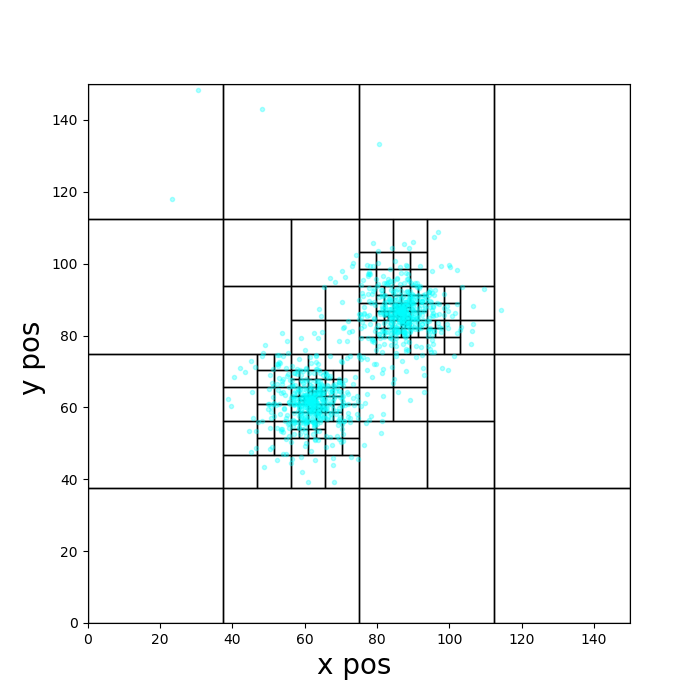
\includegraphics[width=0.9\linewidth]{./plots/quadtree.png}
    \caption{Quadtree plotted.}
    \label{quad}
\end{figure}


\section{Problem 8}
Not implemented. Sad!

Another small rant. I would like it to be known that Computational Astrophysics
is a course based entirely on simulations ($6$ ECs). There were $5$ assignments
that took several weeks to code up---\emph{with} the simulation backbone
already provided (via \texttt{AMUSE}). This problem could probably take a
month to complete on its own. And it is only worth a small fraction of the
final grade. I would love to continue talks on the expectations of this course
in the future.



\end{document}


\section{1}
\subsection{1a}

Here we test our rng as we did in the first handout. 
\begin{figure}[h!]
    \centering
    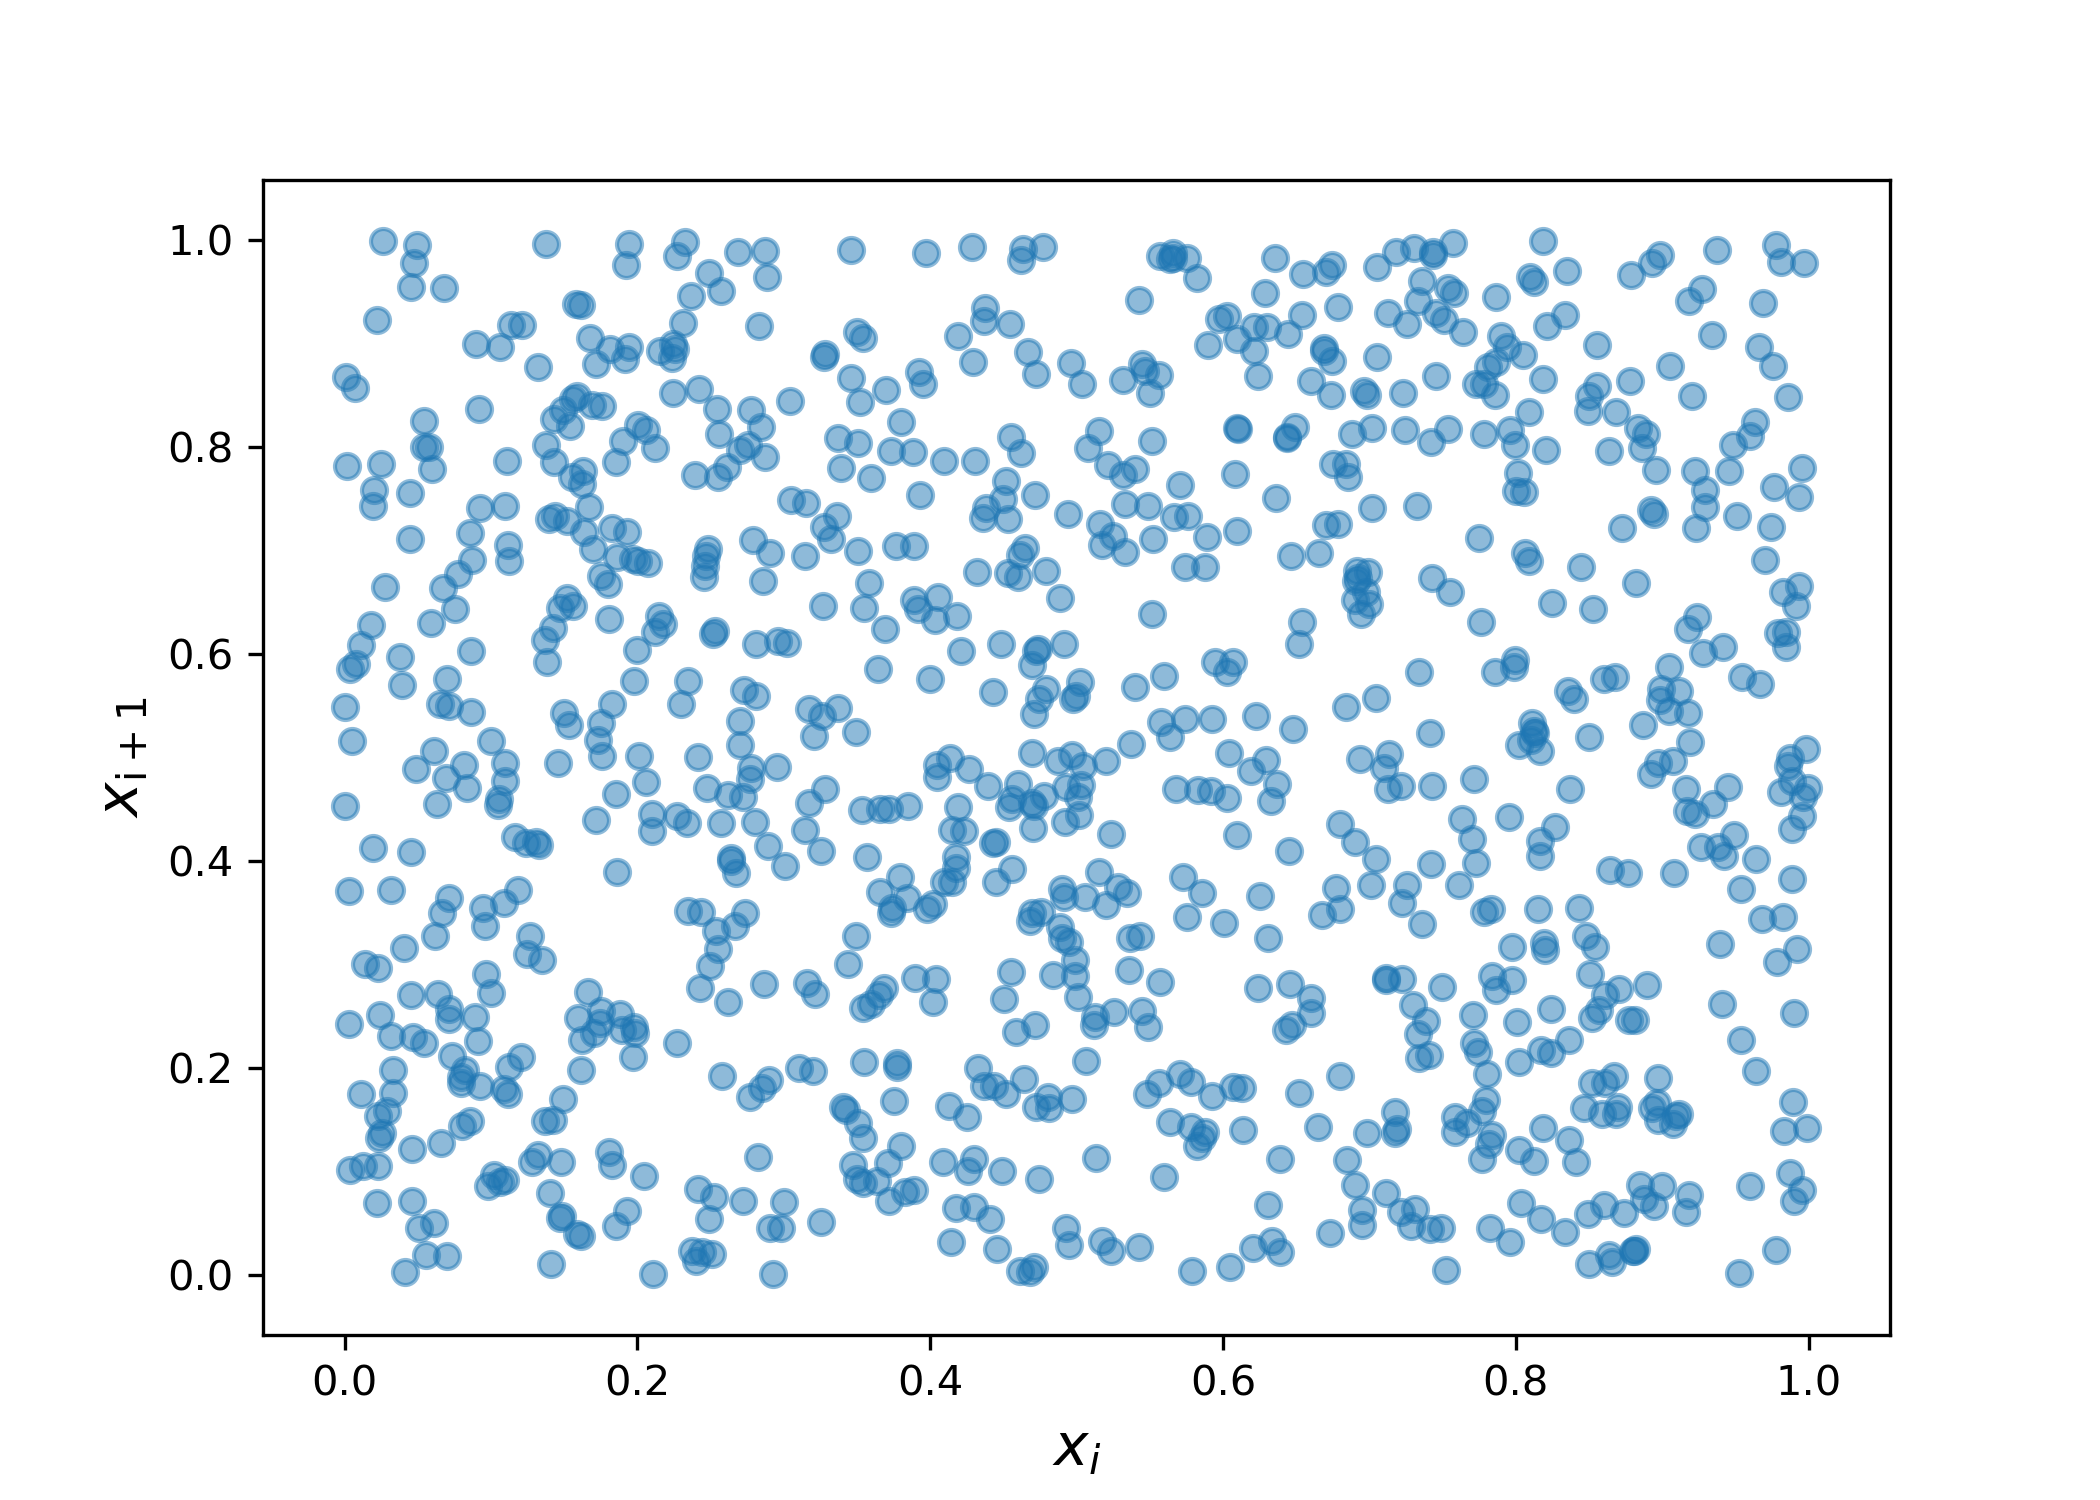
\includegraphics[width=0.9\linewidth]{./plots/x_x_1.png}
    \caption{$x$ vs. $x_{i+1}$ for the random number generator.}
    \label{plt1}
\end{figure}
Looking at the $i$ versus the $i+1$ components of our rng, there appears
to be little correlation between the numbers, which is a good sign. In
\autoref{plt2} we see the values that each number has in the array of 
$1000$ random numbers. It is between $0$ and $1$, also a good sign.
\begin{figure}[h!]
    \centering
    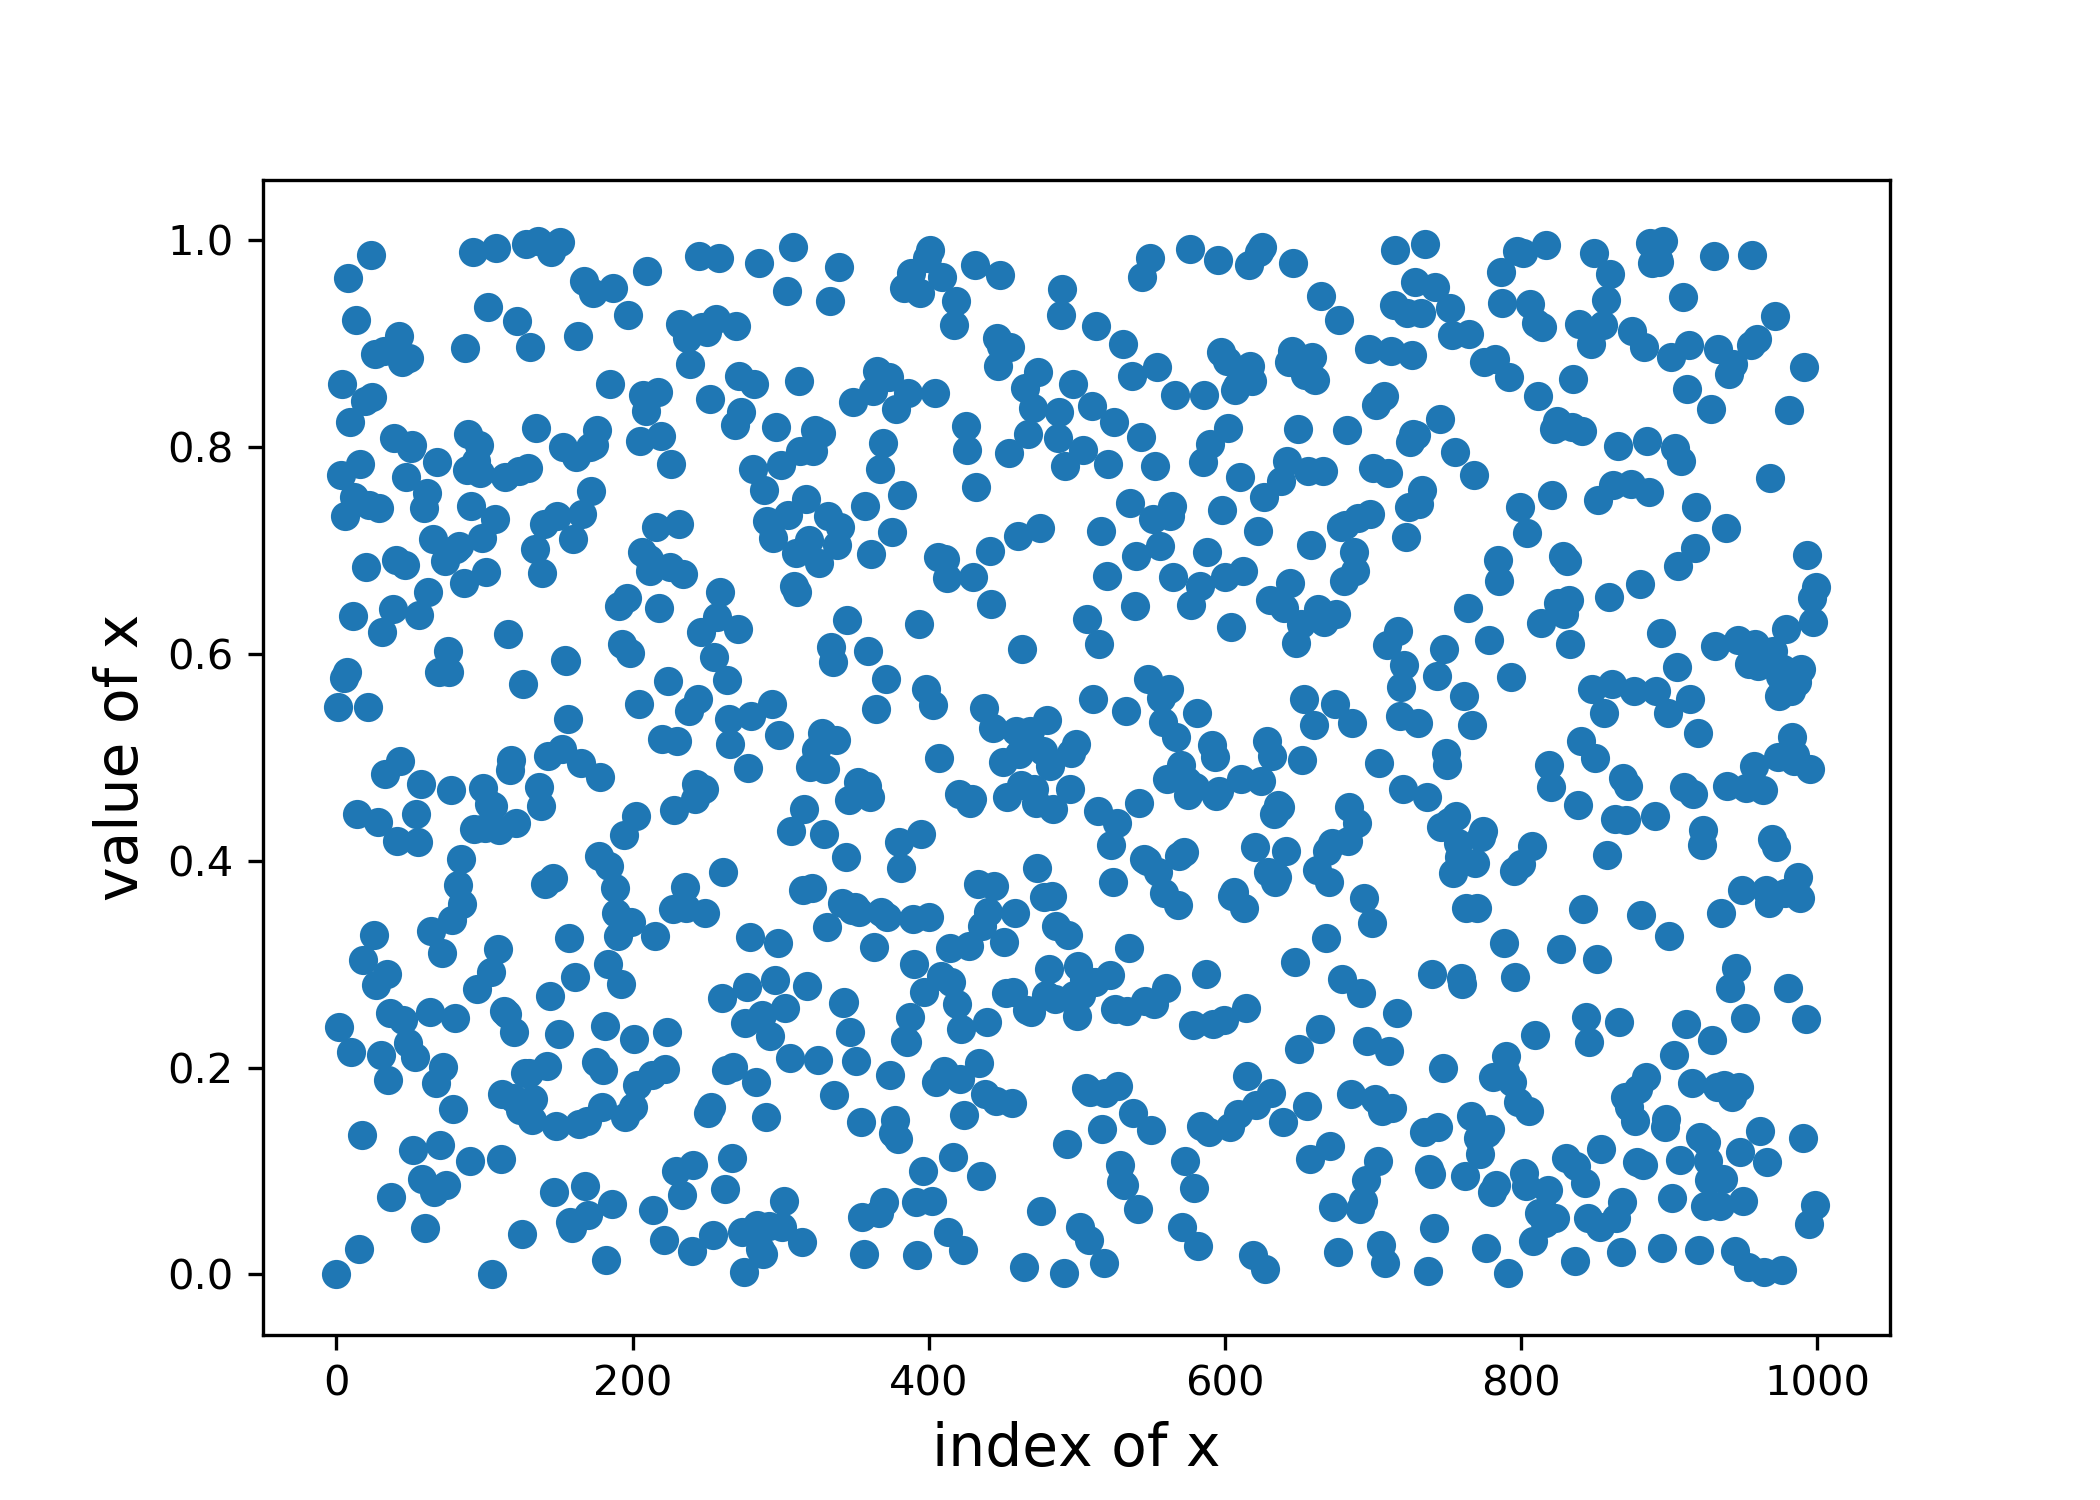
\includegraphics[width=0.9\linewidth]{./plots/xval_xind.png}
    \caption{The value of $x$ at a given index.}
    \label{plt2}
\end{figure}
However, in \autoref{plt3} it is clear something is wrong with the rng.
\begin{figure}[h!]
    \centering
    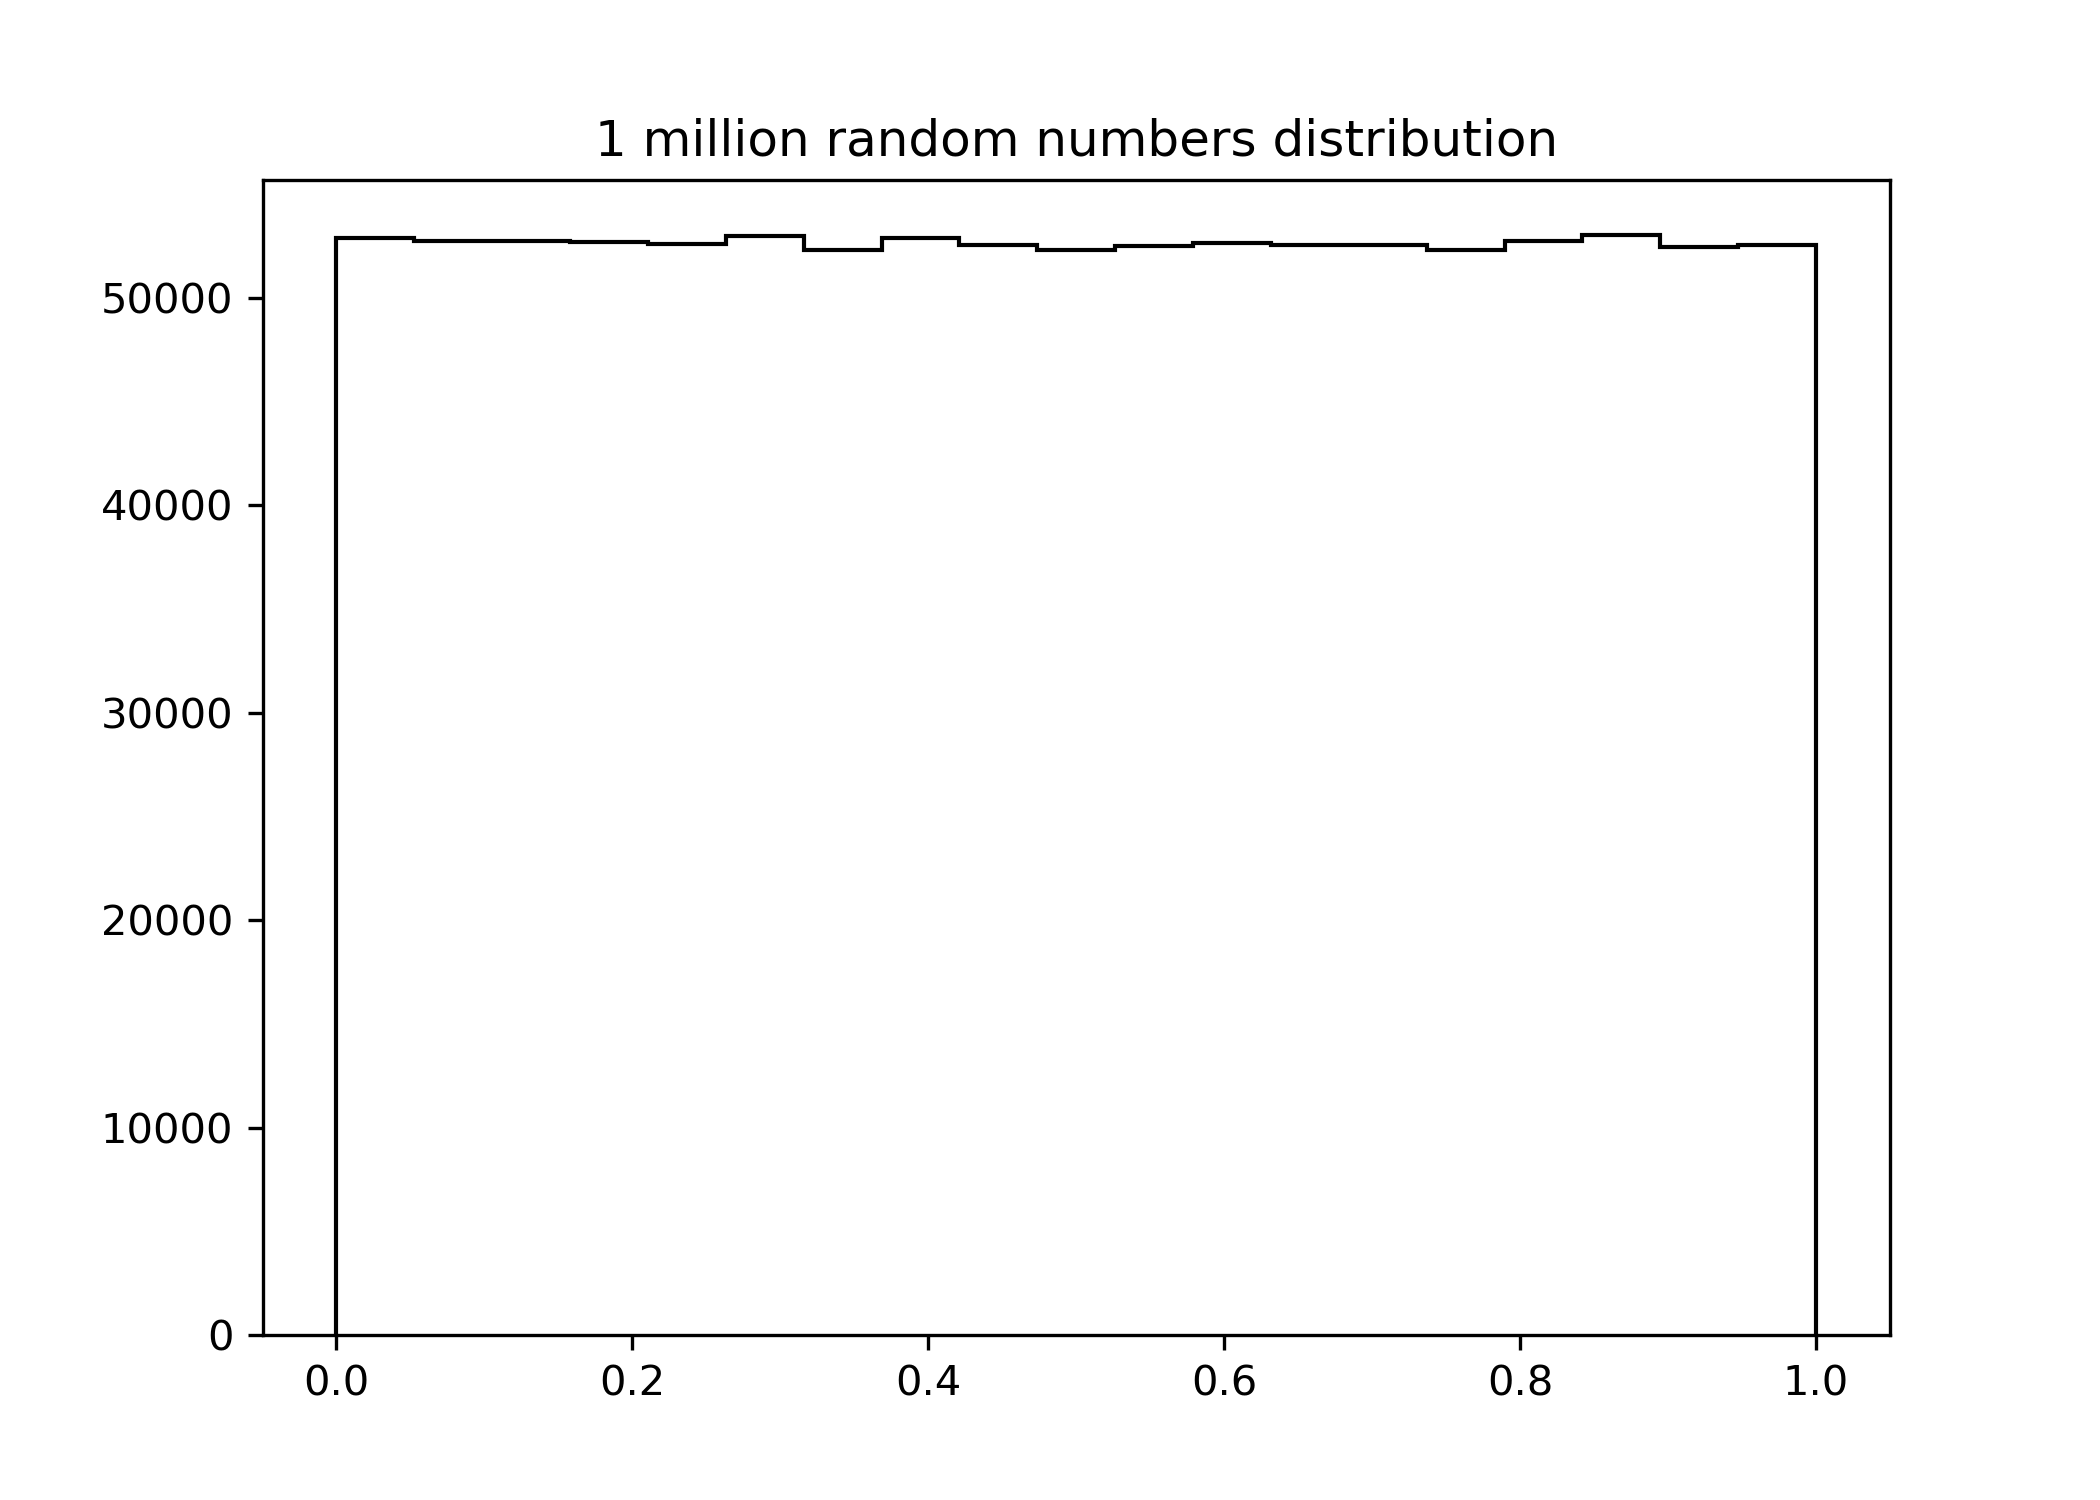
\includegraphics[width=0.9\linewidth]{./plots/1mil_hist.png}
    \caption{$1$ million random numbers plotted.}
    \label{plt3}
\end{figure}
As is plainly seen, the numbers in the random generator nearly all go above 
$5 \times 10^4$, which is not what we would expect from the rng. I am not
sure what the issue is. I attempted to cast all of the values as \texttt{ints}
but I was getting runtime errors in the $XOR$ bit-shift. The variance appears
to be fine, so I left it as is.


\subsection{1b}

\lstinputlisting{p1b.py}

As I have already explained that my rng is likely wrong, I will not mention
it further in the exercise. Here we use the Box-Muller method to generate
a Gaussian distribution, seen in \autoref{plt4}.
\begin{figure}[h!]
    \centering
    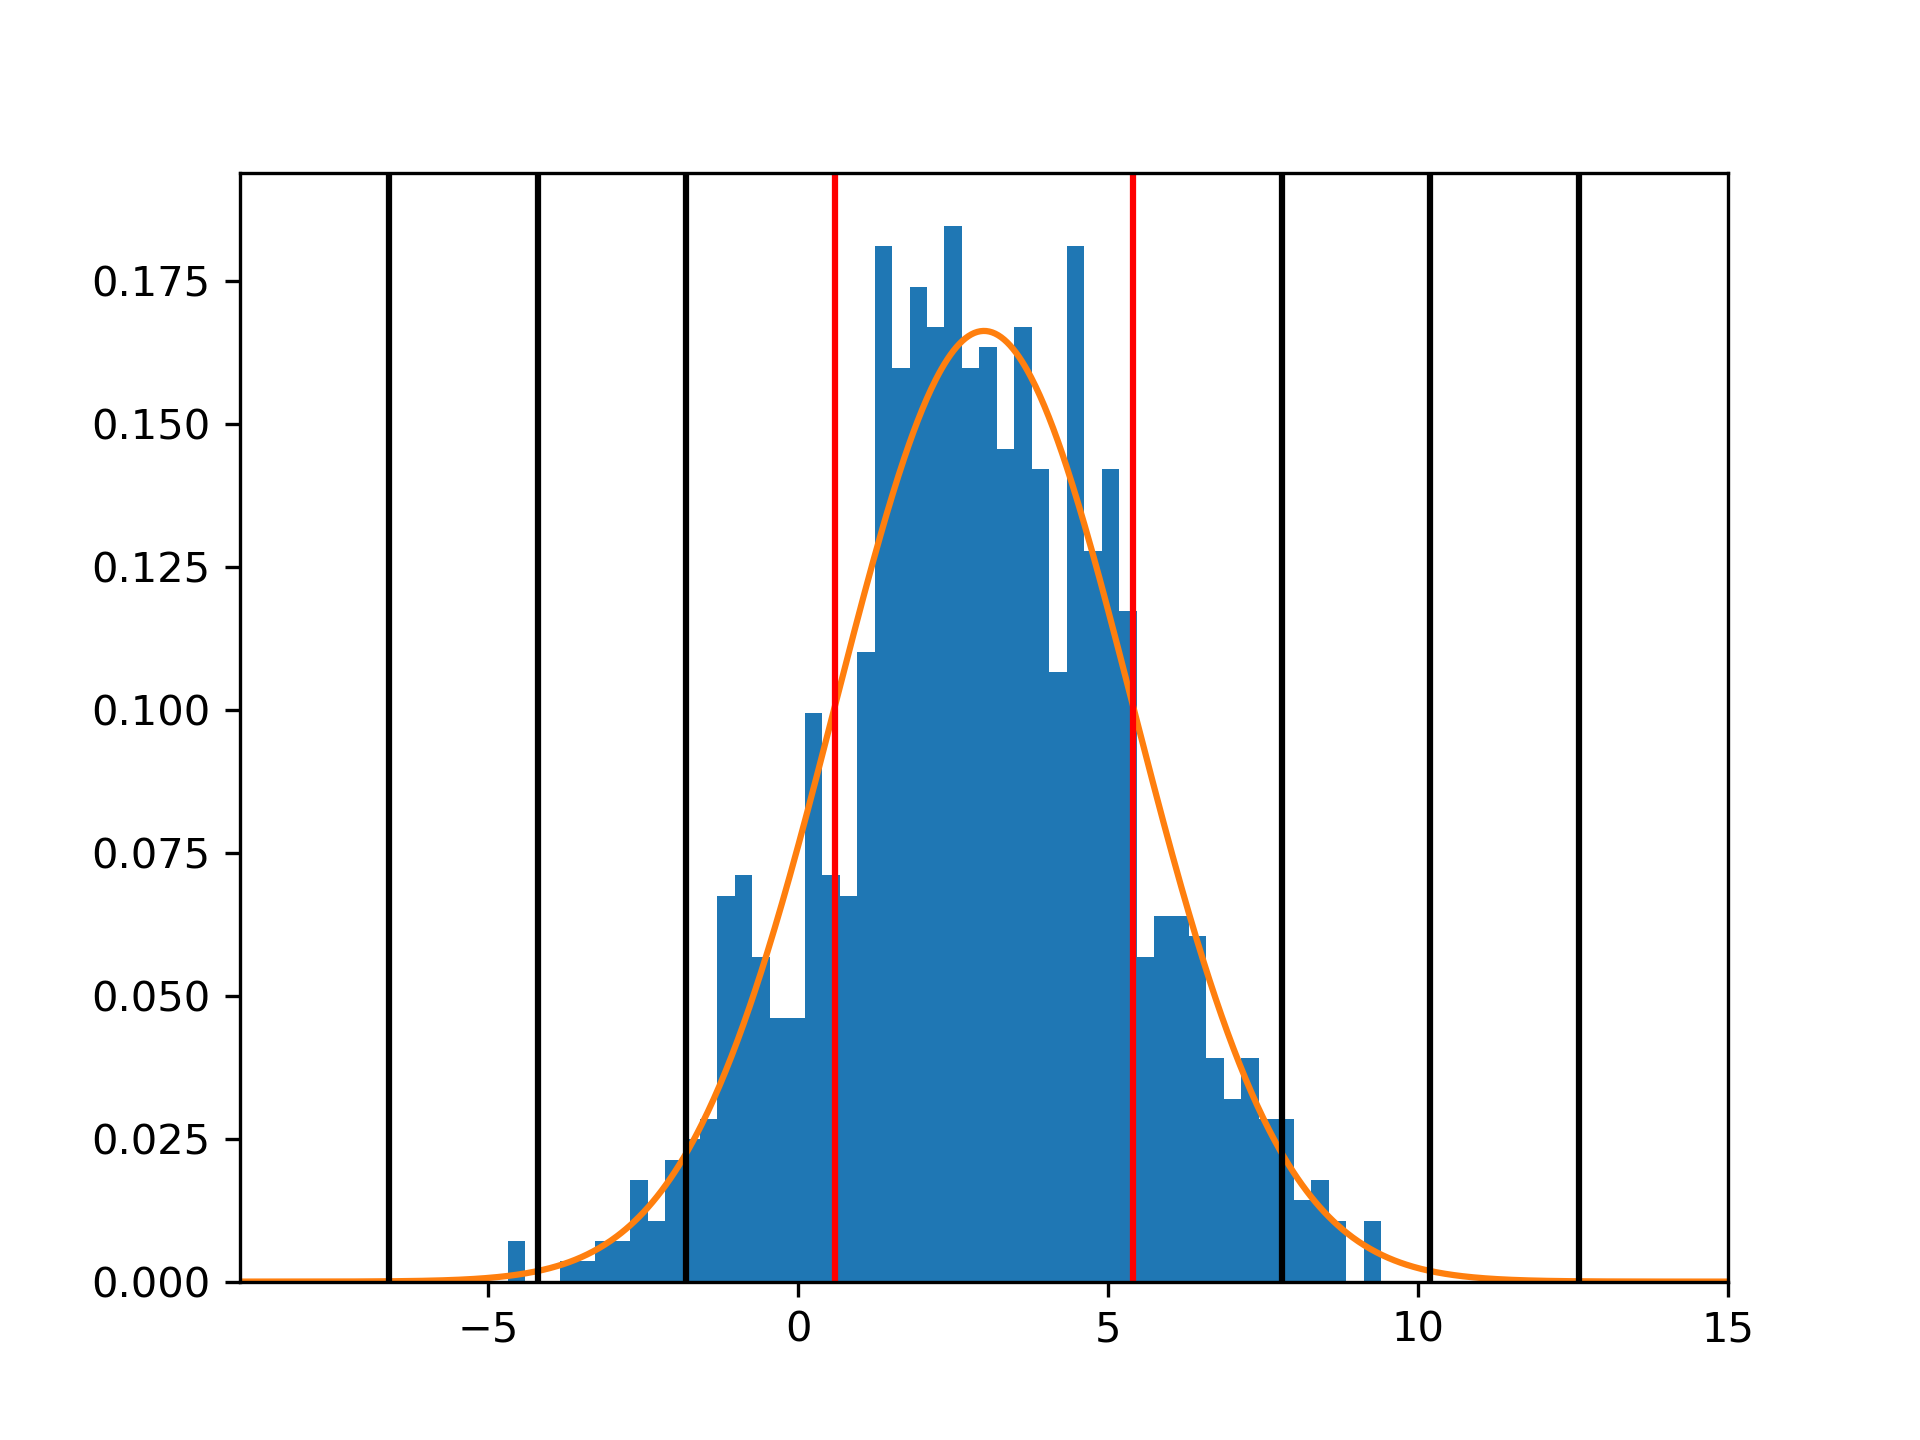
\includegraphics[width=0.9\linewidth]{./plots/box_gauss.png}
    \caption{My distribution with \texttt{numpy.norm} overplotted.}
    \label{plt4}
\end{figure}
The Box-Mueller method seems to work nicely, it is simply the rng that
ruins the Gaussian, given that there are values that are favored in the
$+1\sigma$ range.


\subsection{1c}

\lstinputlisting{p1c.py}
Next is the KS test. For this, I am unsure where I went wrong because
I followed the slides but to no avail. With time constraints, I was not
able to figure it out. Figures are plotted below.
\begin{figure}[h!]
    \centering
    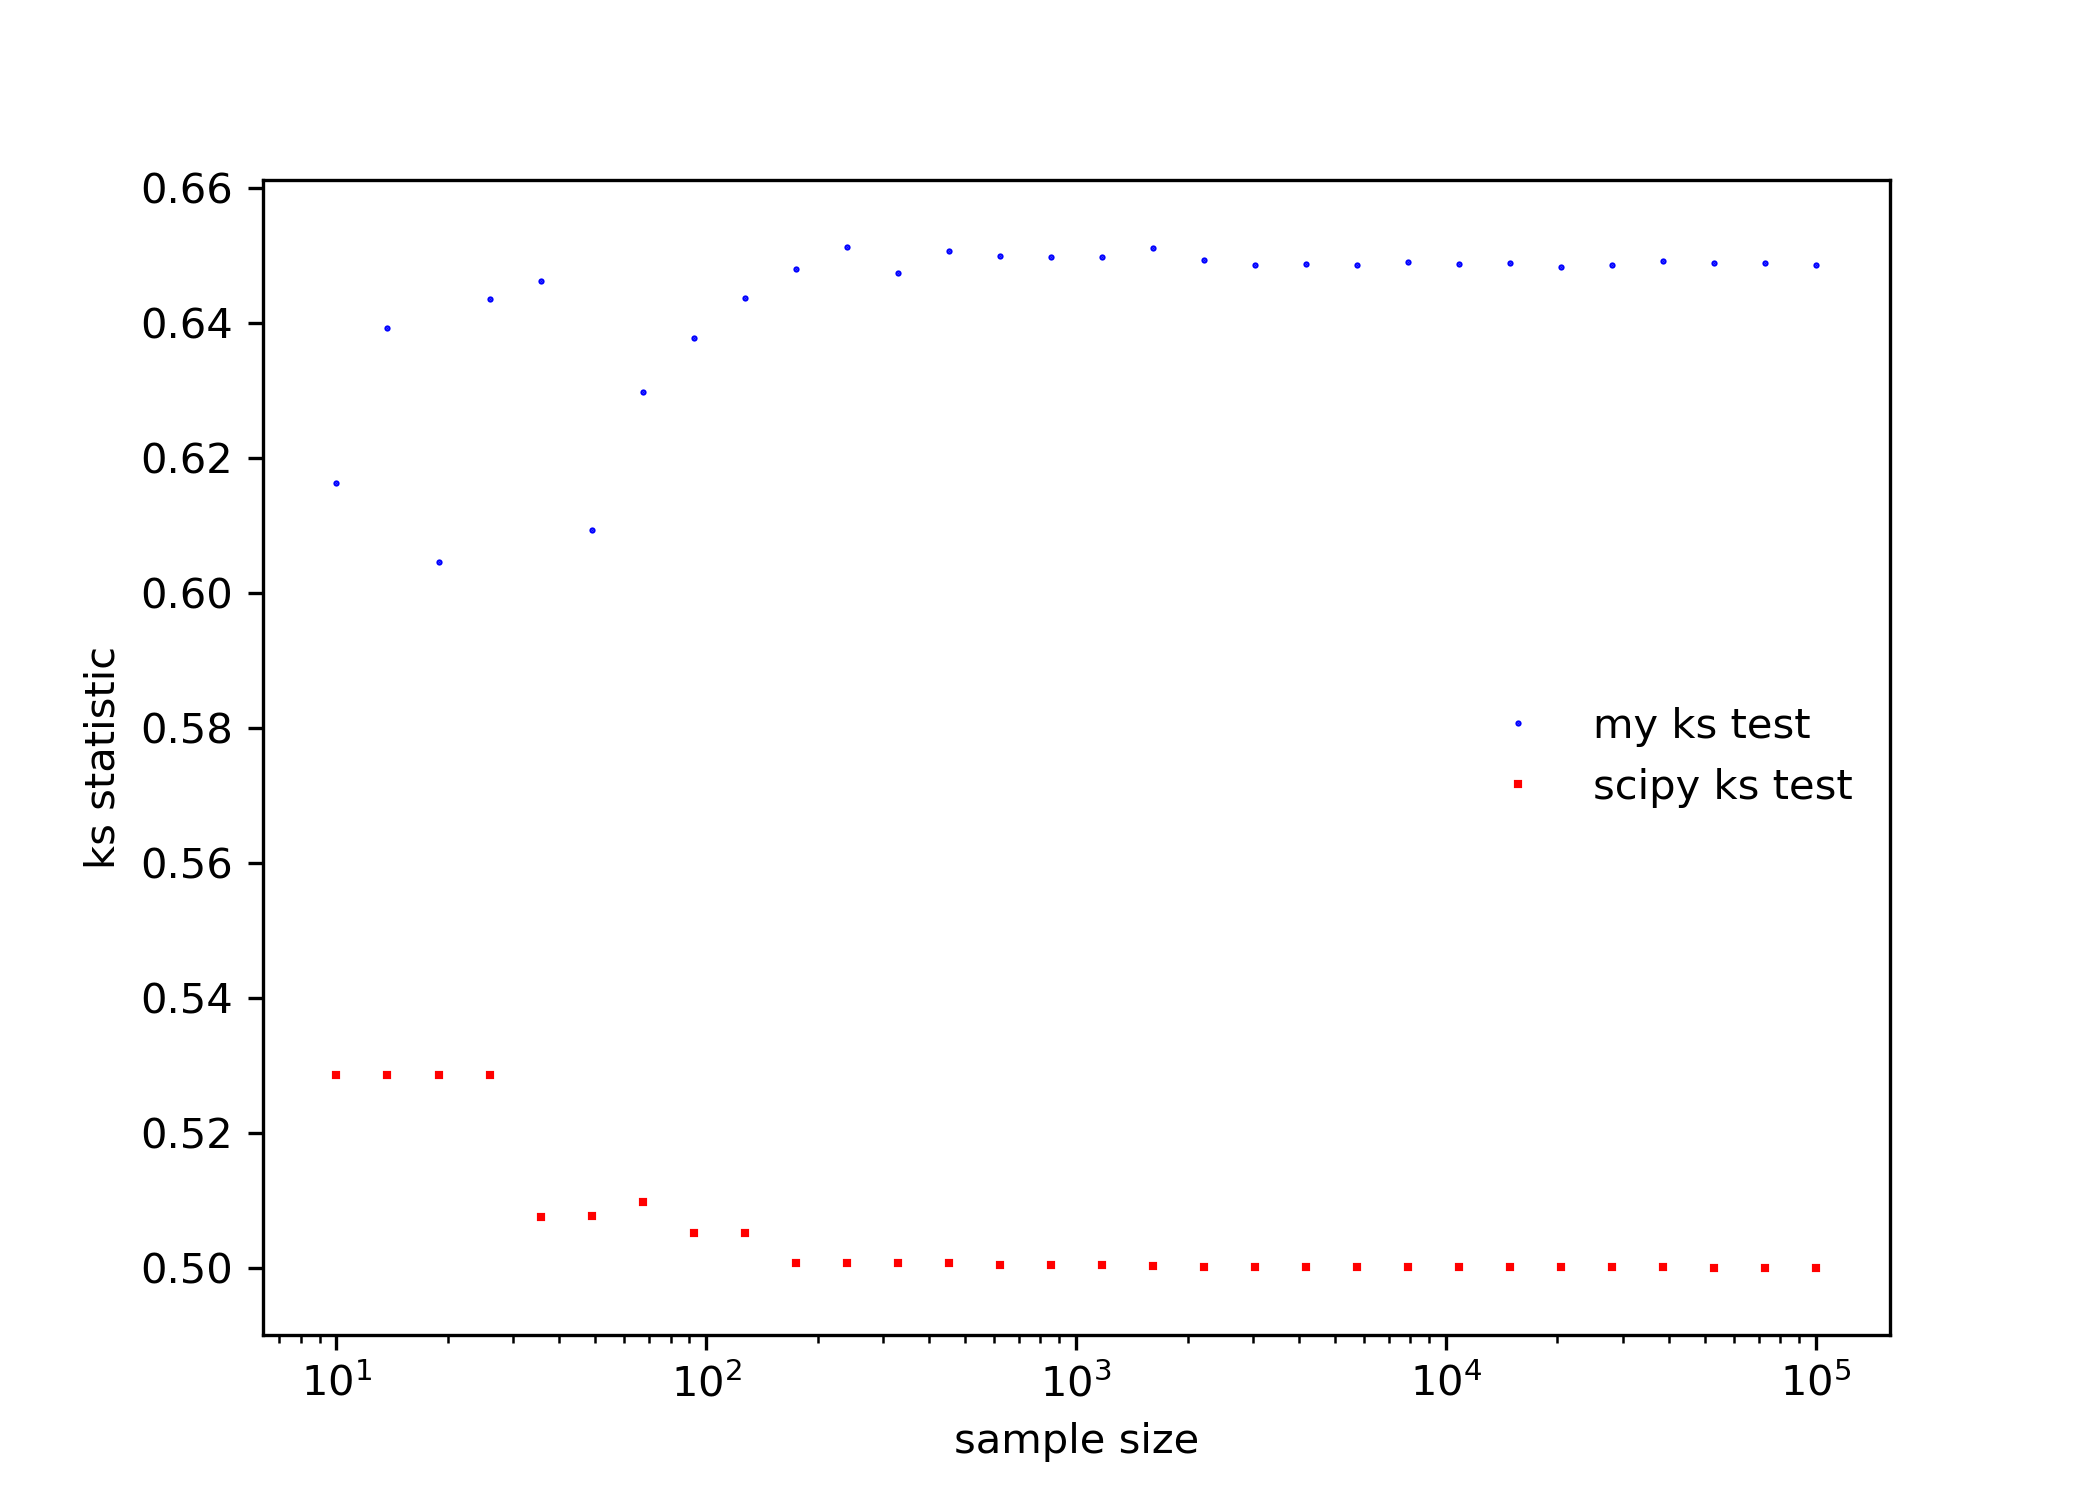
\includegraphics[width=0.9\linewidth]{./plots/ks_stat.png}
    \caption{$1$ million random numbers plotted.}
    \label{plt3}
\end{figure}

\begin{figure}[h!]
    \centering
    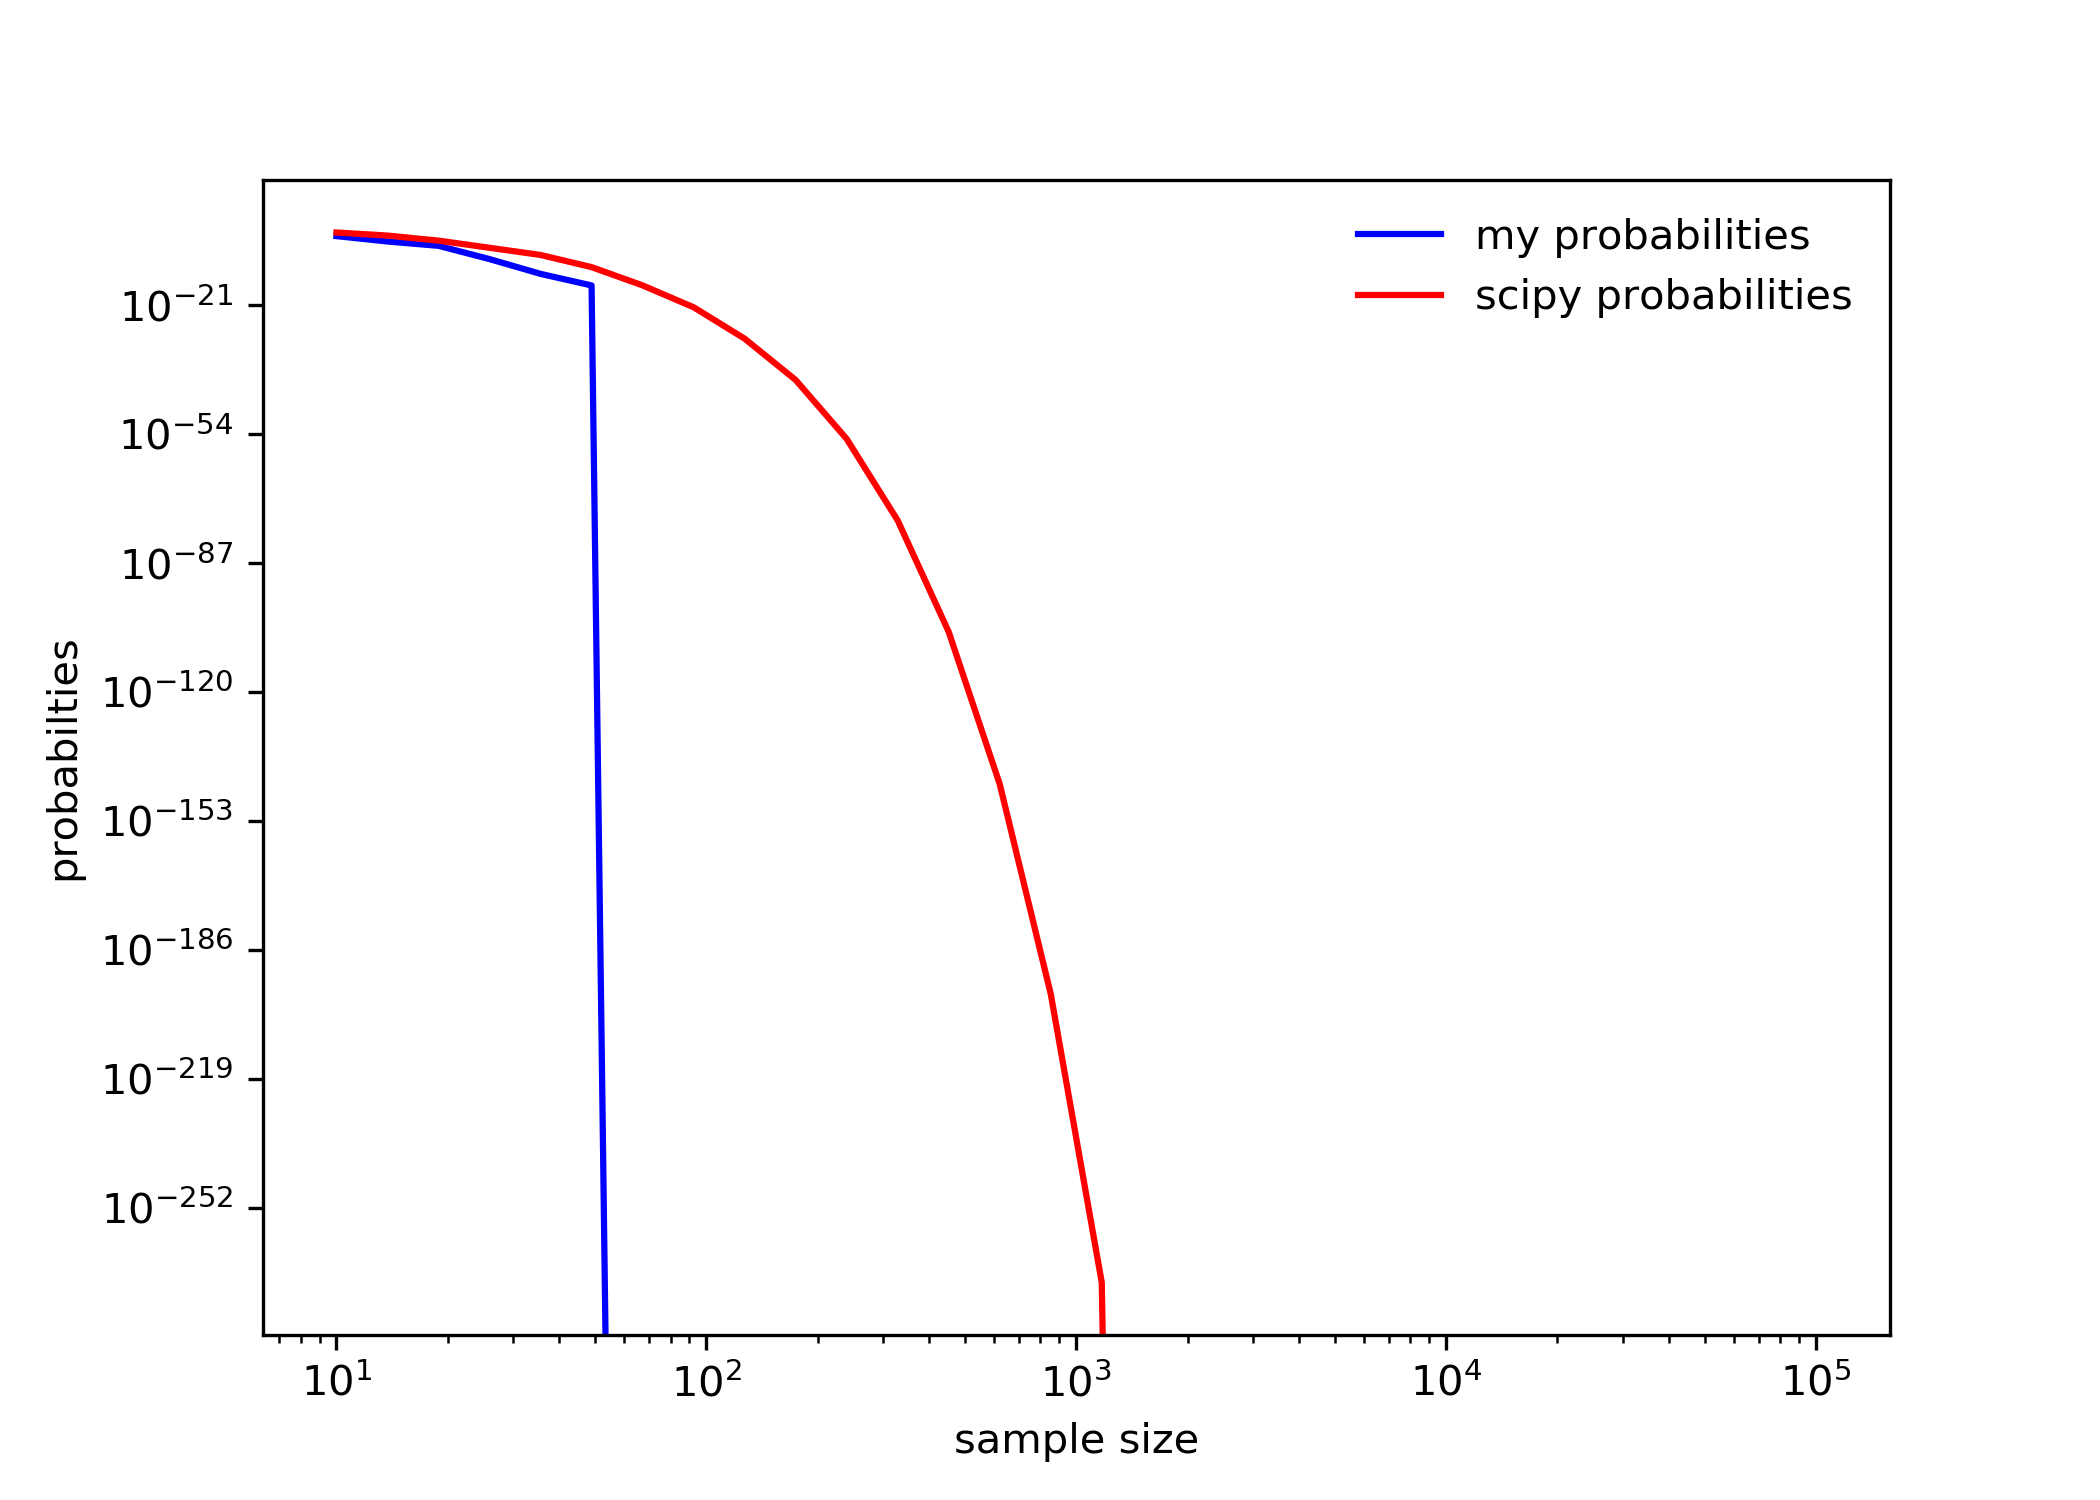
\includegraphics[width=0.9\linewidth]{./plots/ks_prob.png}
    \caption{$1$ million random numbers plotted.}
    \label{plt3}
\end{figure}



\subsection{1d}

\lstinputlisting{p1d.py}
Next is the Kuiper test. As with the KS test, I am unsure where I went wrong
because I followed the slides but to no avail. With time constraints, 
I was not able to figure it out. Figures are plotted below. One obvious 
explanation is that my distribution does not fit a Gaussian.
I am unsure of potential (and likely) bugs in my code.
\begin{figure}[h!]
    \centering
    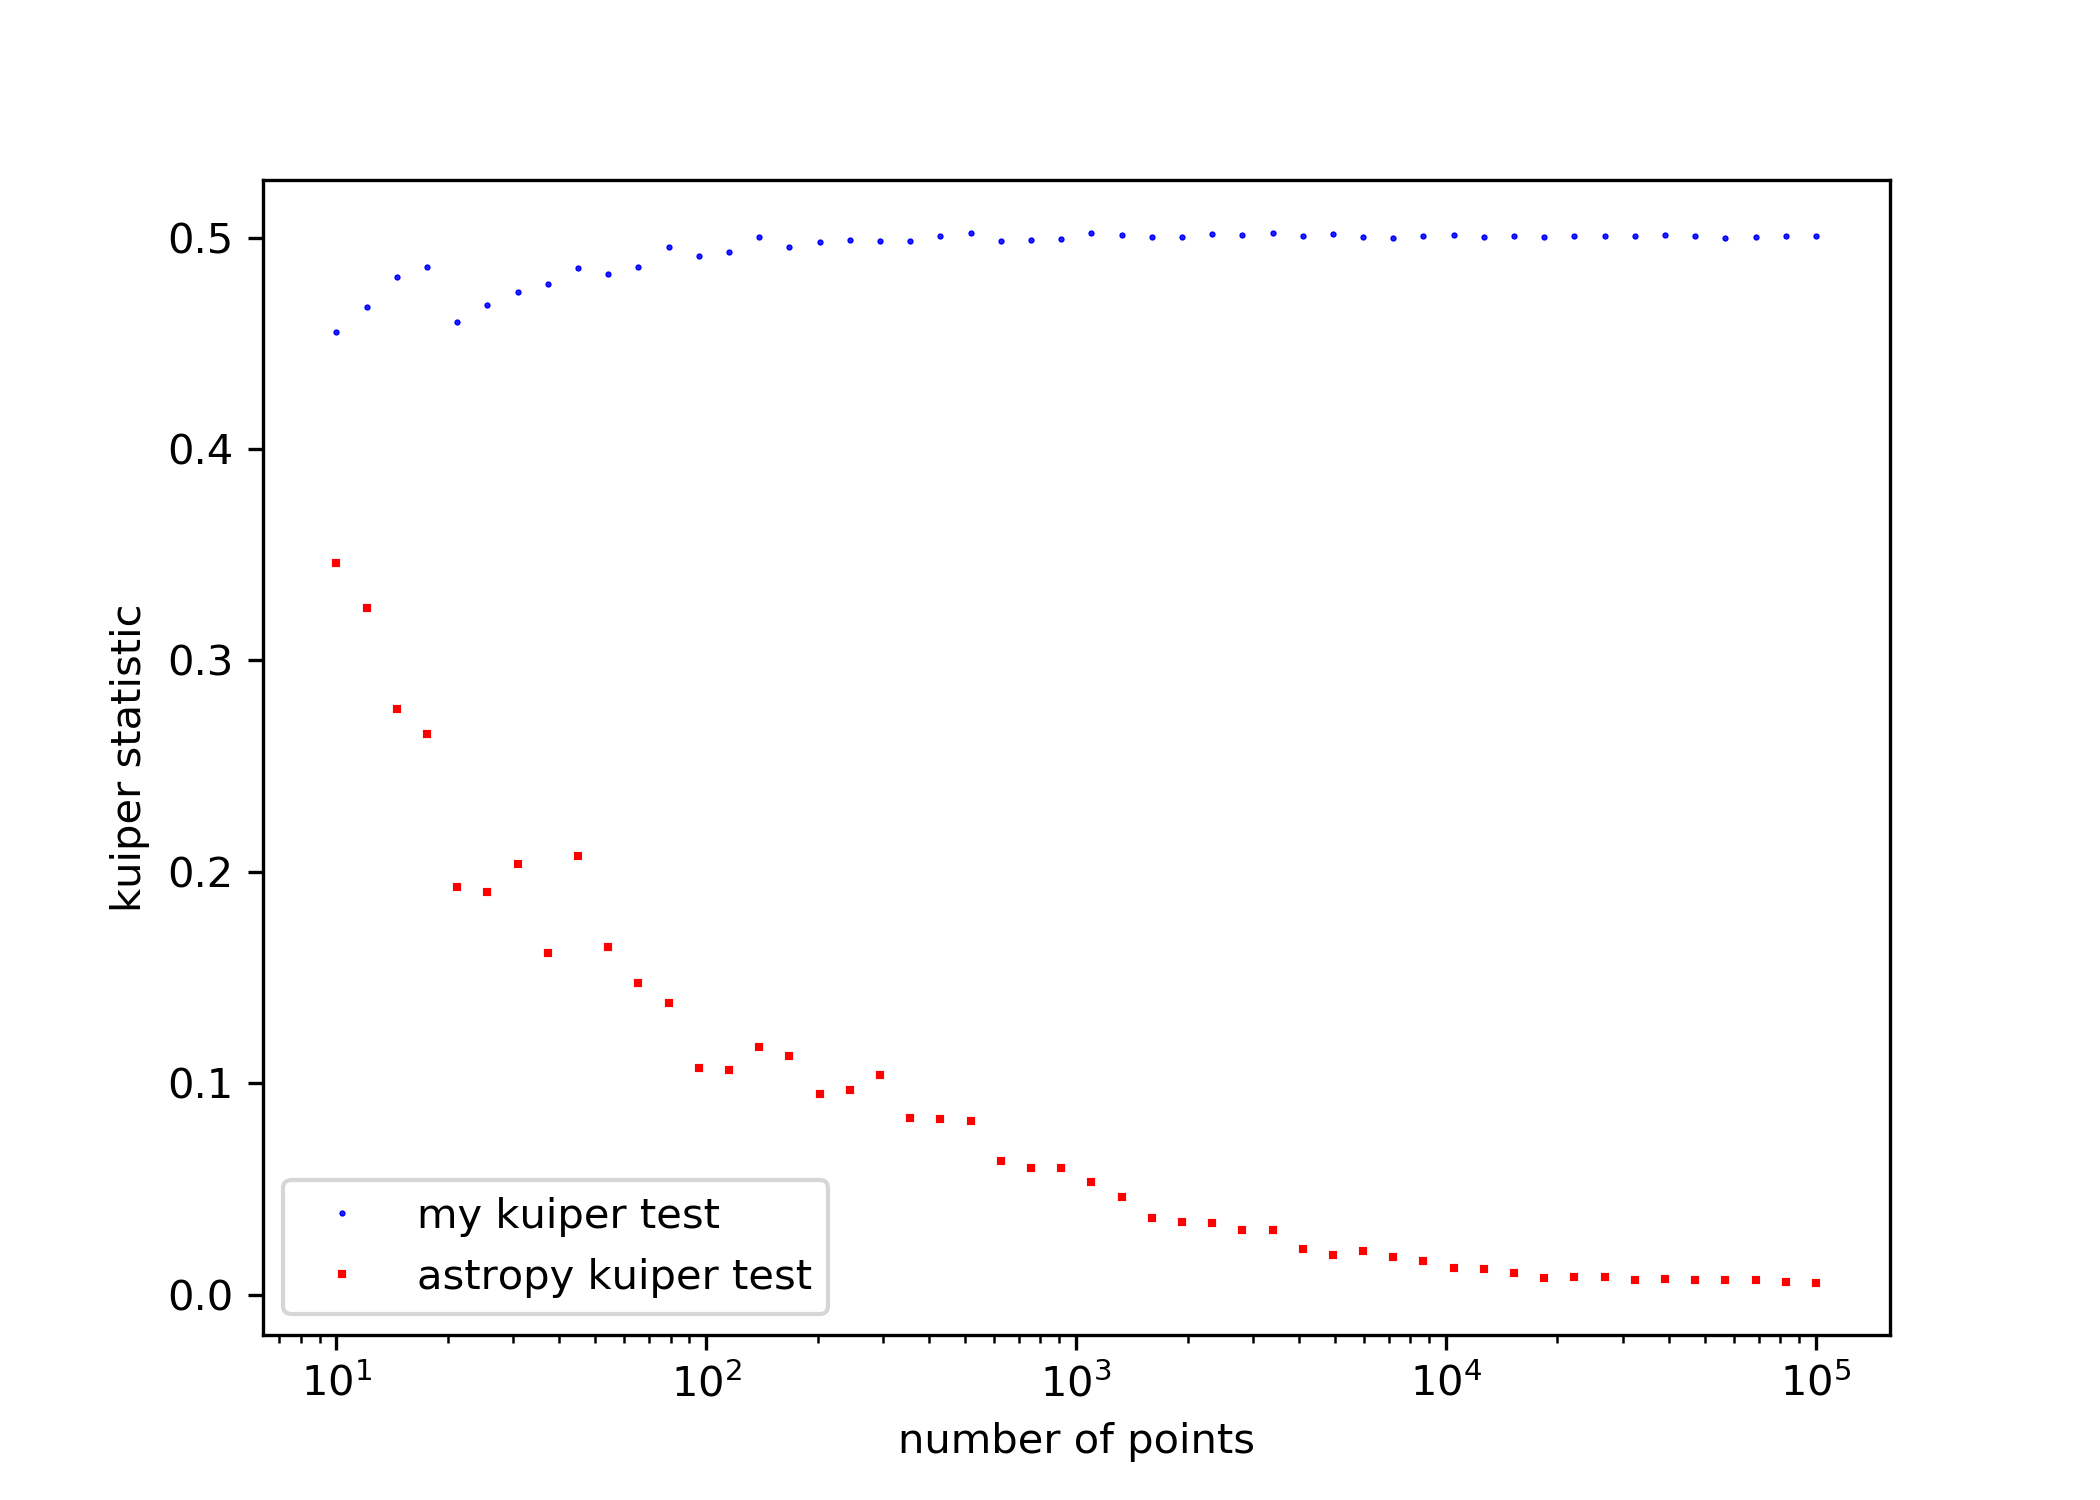
\includegraphics[width=0.9\linewidth]{./plots/kuiper_stat.png}
    \caption{Kuiper distance statistic.}
    \label{kuip_s}
\end{figure}

\begin{figure}[h!]
    \centering
    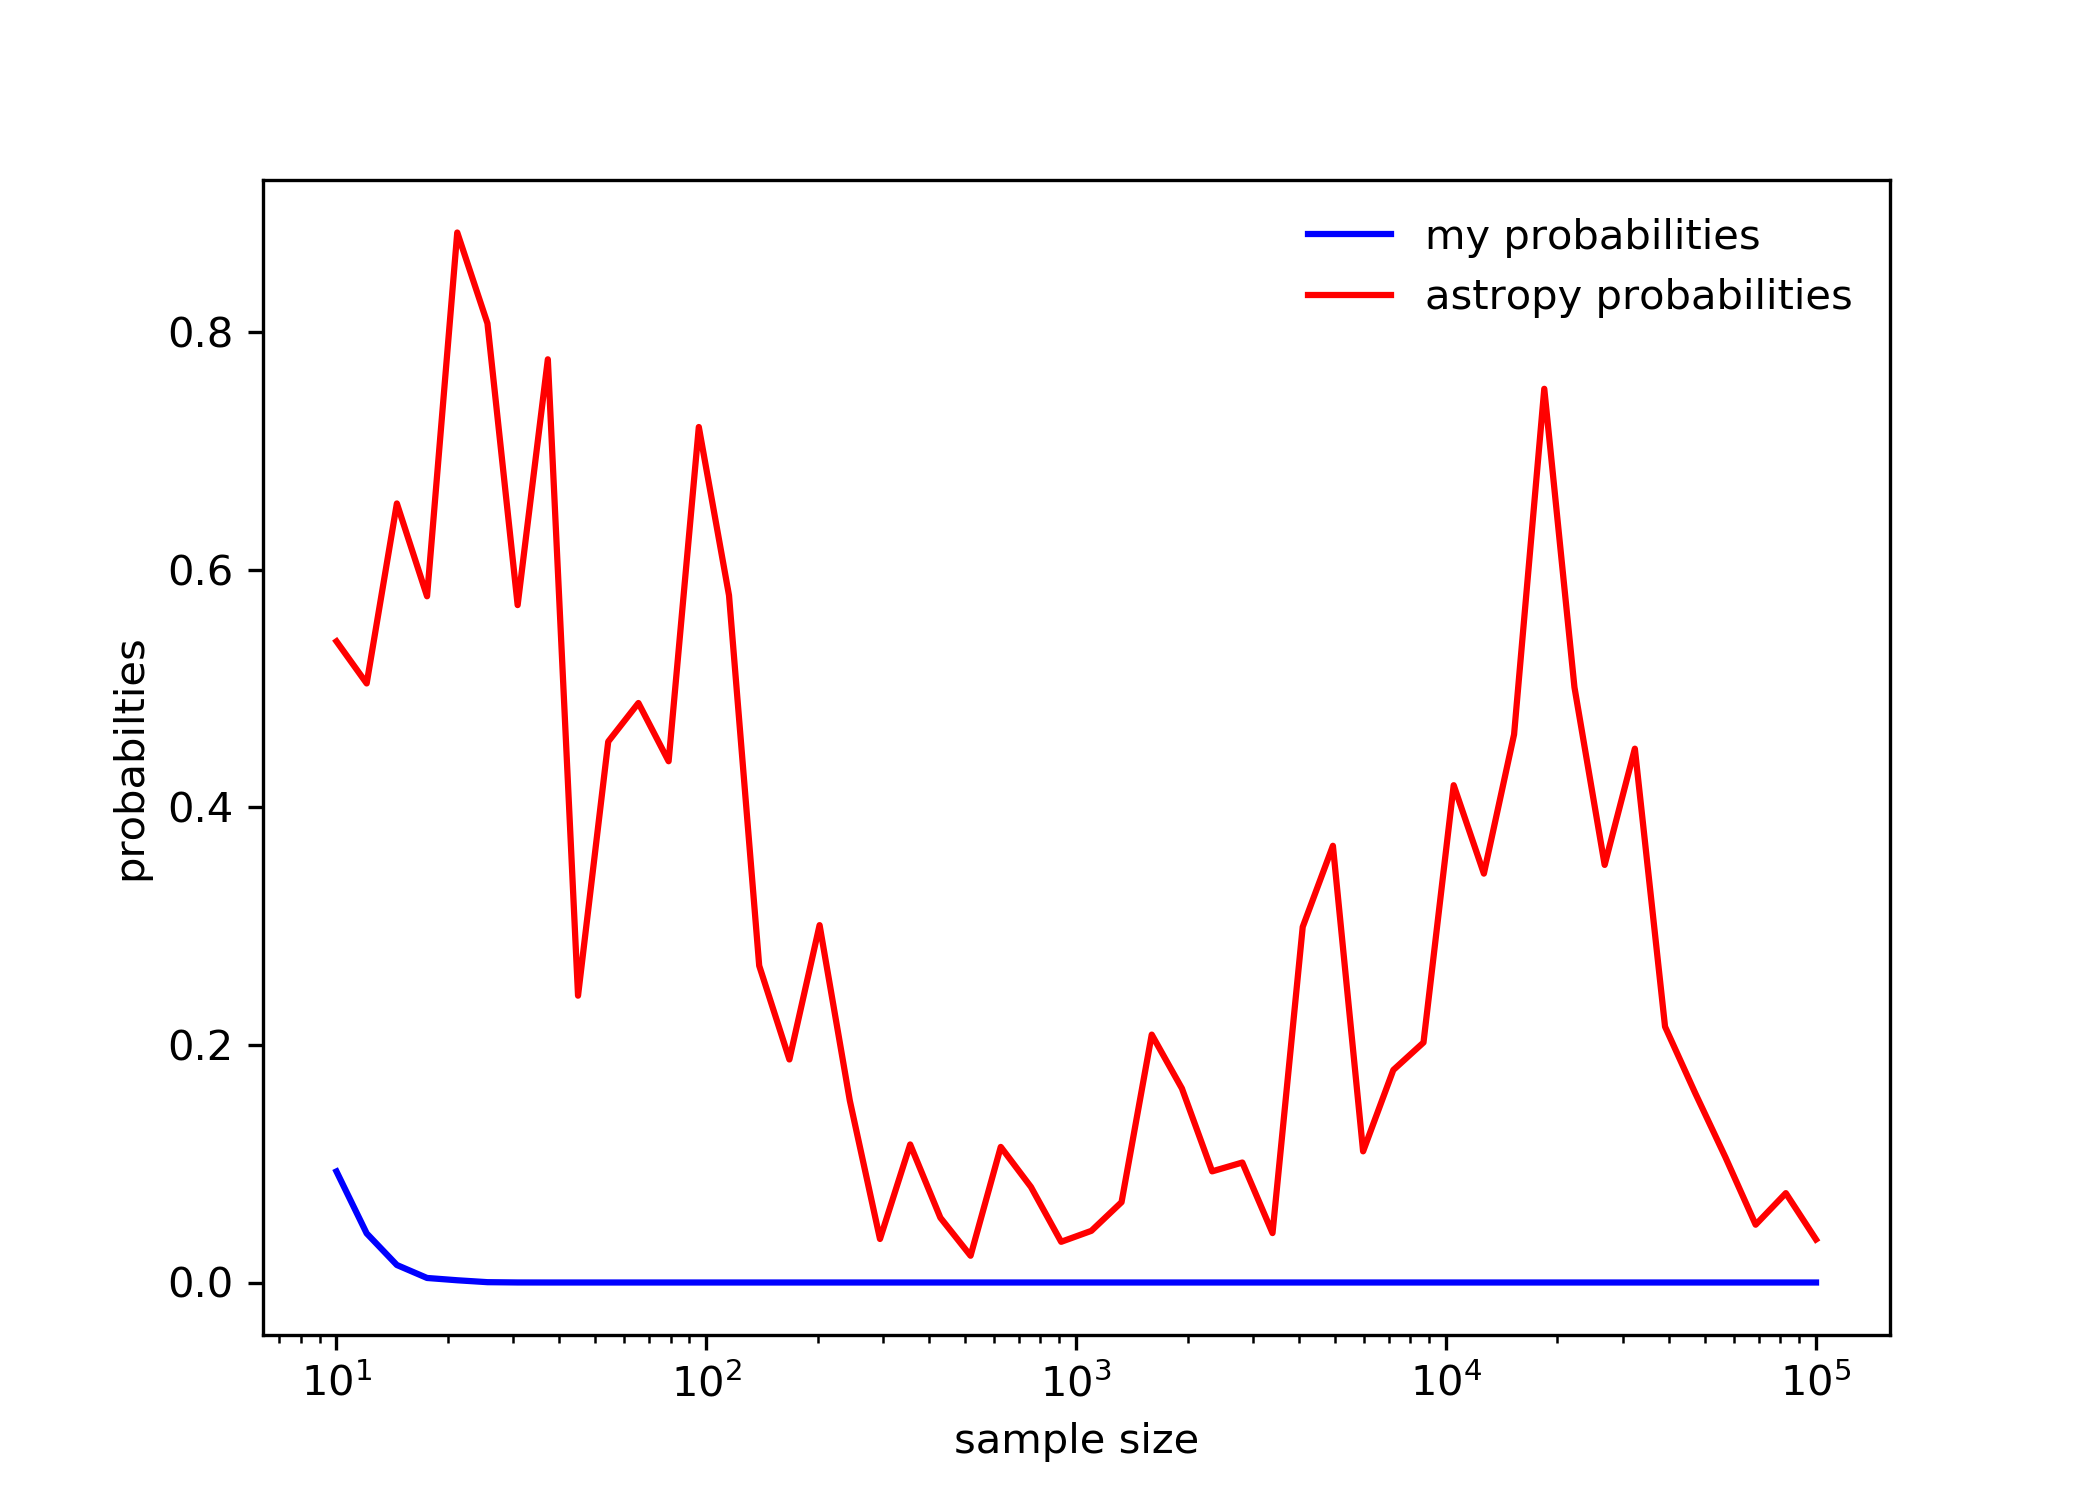
\includegraphics[width=0.9\linewidth]{./plots/k_prob.png}
    \caption{Kuiper probabilities.}
    \label{kuip_p}
\end{figure}



\subsection{1e}

\lstinputlisting{p1e.py}
Next, we are meant to verify a statistic of our choice (in this case the 
KS statistic) with a set of random numbers. I recognized too late that I need
to implement a $2$D KS sampler. As can be seen, I have a potential CDF to use,
but the statistic cannot be used at this time.



\section{Problem 2}

\lstinputlisting{p2.py}
We set out to make initial density fields based off of the power spectrum,
\begin{equation}
  P(k) = k^n,
\end{equation}
where $n$ is $-1, -2, -3$. Essentially, we setup the indices for the Fast
Fourier Transform (FFT) as described in the slides. We define the function
for the power spectrum, use our rng to make random numbers, and finally
perform the FFT on each field. Figures are plotted below.

\begin{figure}[h!]
    \centering
    \includegraphics[width=0.9\linewidth]{./plots/gauss_field_n_1.png}
    \caption{Gaussian field for $n=-1$.}
    \label{gf1}
\end{figure}
The initial field in \autoref{gf1} looks roughly what we expect.
Admittedly, I am unsure exactly what is expected, but as the handout
explains, dispersion is dependent on $n$. In \autoref{gf2} we can see
the dispersion causes a bit more ``clumpiness'' (that is, high-density
pockets). In \autoref{gf3}, we see an even higher contrast between
the low-high density regions. (Sorry, my colorbar was not working! It's 
viridis colormap, though.)
\begin{figure}[h!]
    \centering
    \includegraphics[width=0.9\linewidth]{./plots/gauss_field_n_2.png}
    \caption{Gaussian field for $n=-2$.}
    \label{gf2}
\end{figure}
However, in \autoref{gf3} it is clear something is wrong. The physical
distances are not changing as a function of $n$. As $P_k$ changes from
$n=-1$ to $n=-2$ for example, the maximum and minimum k values should increase
from $n=-1$ to $n=-2$. The physical distances should be larger as well.
Given time constraints, I gave up and left the plots as is. I assume 
it has a $2$-fold issue: my rng and perhaps the amplitudes are not actually
changing as expected.
\begin{figure}[h!]
    \centering
    \includegraphics[width=0.9\linewidth]{./plots/gauss_field_n_3.png}
    \caption{Gaussian field for $n=-3$.}
    \label{gf3}
\end{figure}



\section{Problem 3}

\lstinputlisting{p3.py}
We set out to solve the given ordinary differential equation (ODE) given in
the handout. I have very little to show--I do not have the analytic solution,
and it is clear from \autoref{rk} that the solution is not correct. My attempt
was to decompose the second-order ODE to a first-order, then to use the
Runge-Kutta fourth-order algorithm to solve the ODE. Results are below.
I needed much more help than I sought out, I recognize that. But, it was also
important to try and do the rest of the assignment as well...

\begin{figure}[h!]
    \centering
    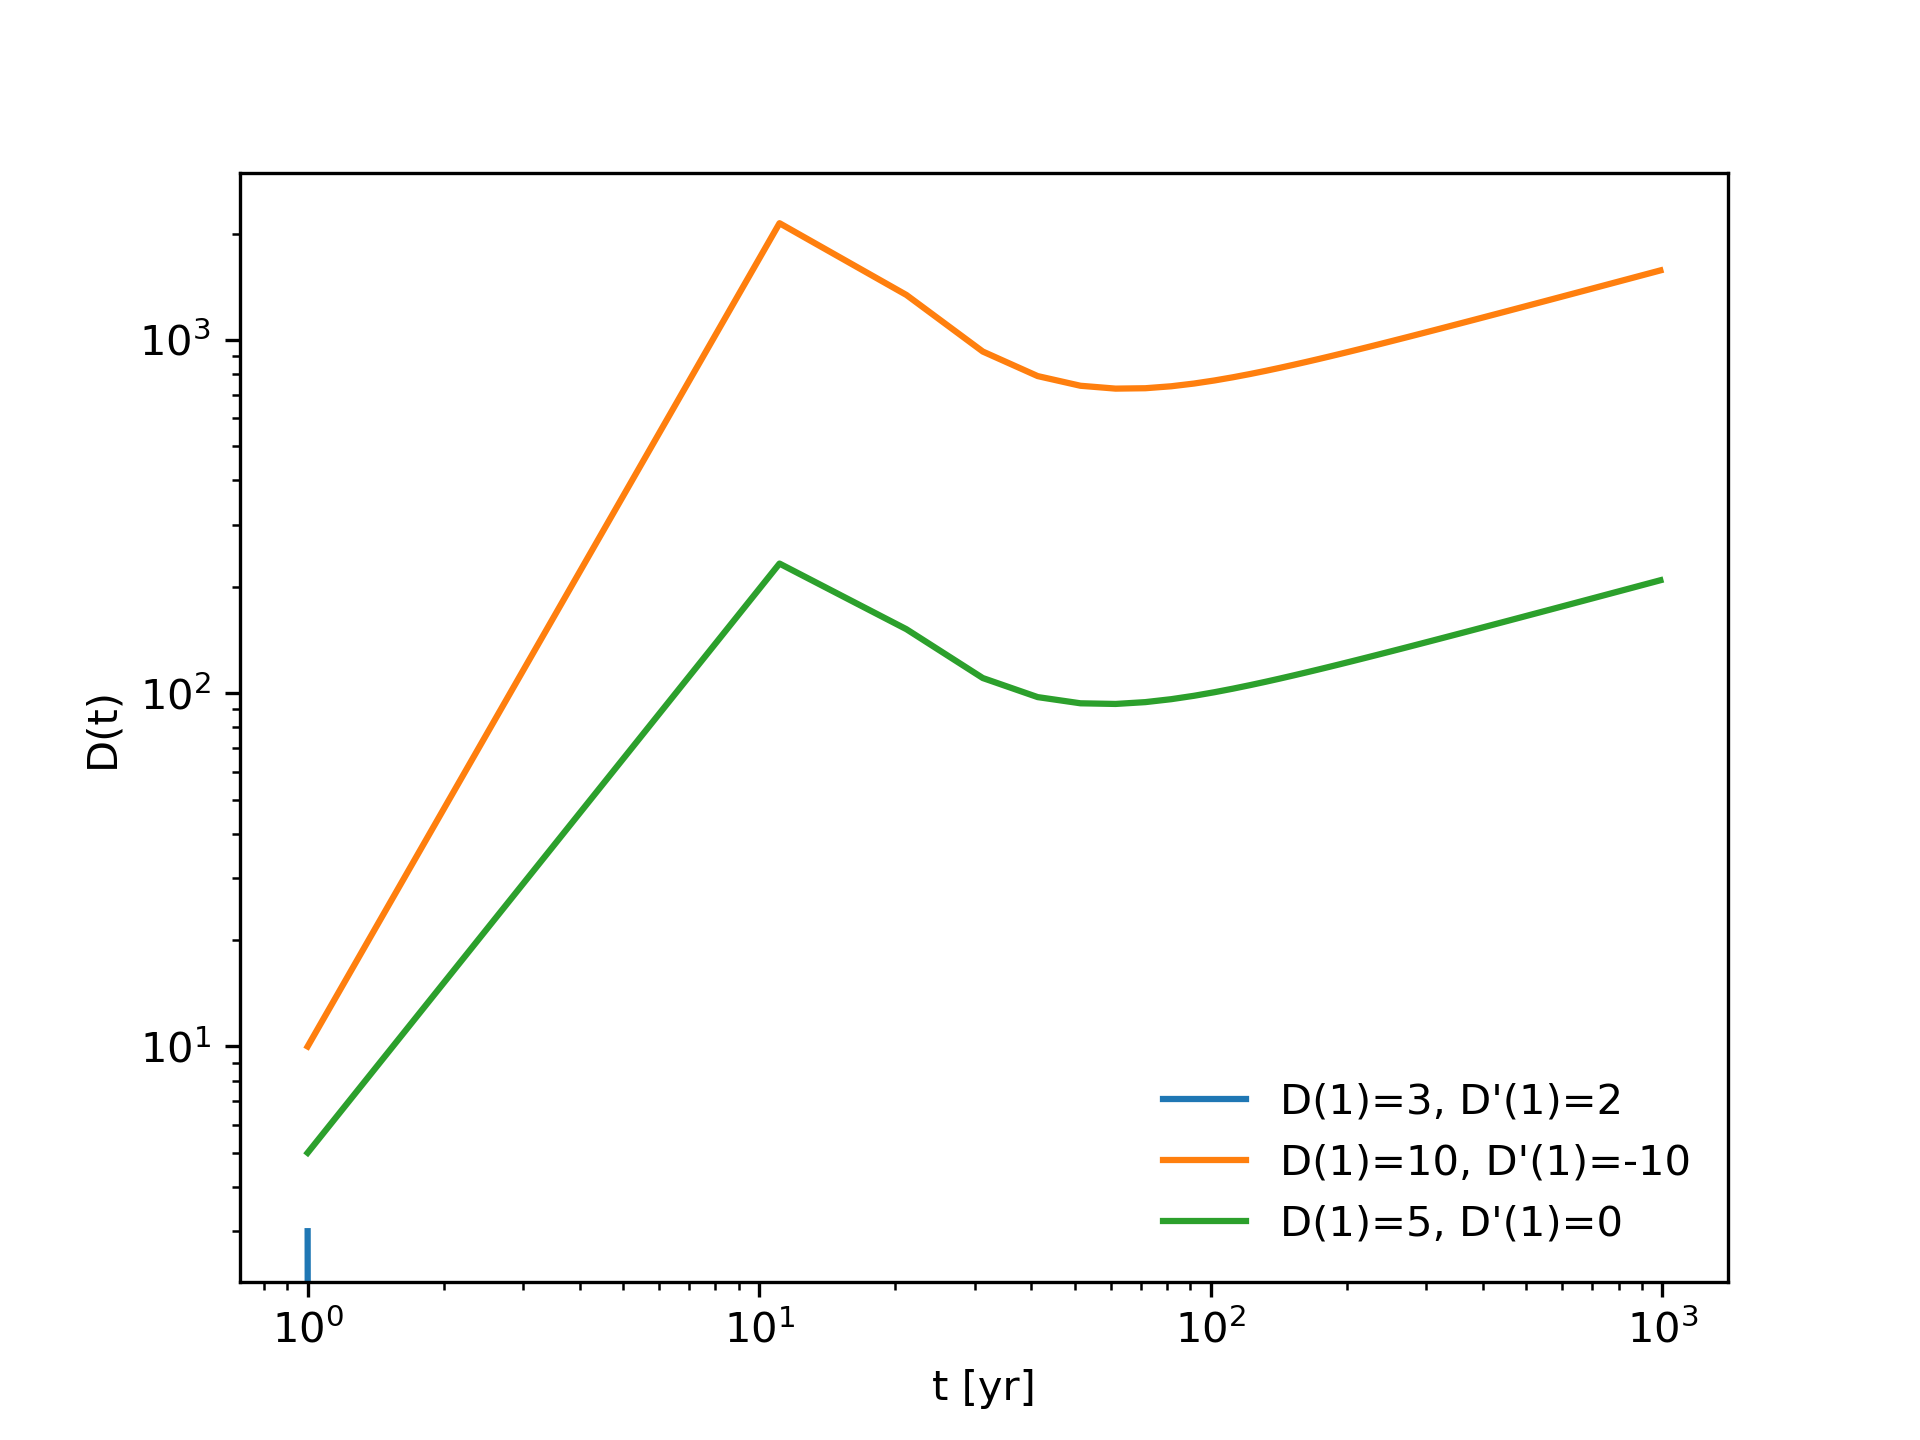
\includegraphics[width=0.9\linewidth]{./plots/rk4.png}
    \caption{Sad plot of the ODE solved.}
    \label{rk}
\end{figure}



\section{Problem 4}
\subsection{4a}

\lstinputlisting{p4a.py}
\lstinputlisting{p4a.txt}
We use the midpoint rule to calculate the desired integral. We achieve only
$1 \times 10^{-4}$ precision. We also use a bound that is sufficiently large
but is not actually $\inf$. A more robust integration is required to get
desired results.




\subsection{4b}

\lstinputlisting{p4b.py}
\lstinputlisting{p4b.txt}
We use the midpoint rule to calculate the desired integral again, but in terms
of the scale factor $a$. We give the value of the analytic derivative of the
linear growth factor at redshift $z=50$ ($a = \frac{1}{51}$),
\begin{equation}
 \dot D(t) = \frac{dD}{da}\dot a,
\end{equation}
using the integral we calculated numerically. The derivative is,
\begin{equation}
 \dot D(t) = \frac{-15}{4}\Omega_m^2 H_0 \frac{I}{a_{\textrm{f}}^3},
\end{equation}
where $\Omega_m$ is the matter density, $H_0$ the Hubble constant,
$a_{\textrm{f}}$ the final scale factor, and $I$ the integral given by,
\begin{equation}
 \int_{a=0}^{a=\frac{1}{51}} \frac{\frac{1}{a^3}}
   {\frac{\Omega_{\textrm{m}}{a^3} + \Omega_{\Lambda}}},
\end{equation}
where $\Omega_{\Lambda}$ is the cosmological constant.


\subsection{4b}

\lstinputlisting{p4b.py}
\lstinputlisting{p4b.txt}
We use the midpoint rule to calculate the desired integral again, but in terms
of the scale factor $a$. We give the value of the analytic derivative of the
linear growth factor at redshift $z=50$ ($a = \frac{1}{51}$),
\begin{equation}
 \dot D(t) = \frac{dD}{da}\dot a,
\end{equation}
using the integral we calculated numerically. The derivative is,
\begin{equation}
 \dot D(t) = \frac{-15}{4}\Omega_m^2 H_0 \frac{I}{a_{\textrm{f}}^3},
\end{equation}
where $\Omega_m$ is the matter density, $H_0$ the Hubble constant,
$a_{\textrm{f}}$ the final scale factor, and $I$ the integral given by,
\begin{equation}
 \int_{a=0}^{a=\frac{1}{51}} \frac{\frac{1}{a^3}}
   {\frac{\Omega_{\textrm{m}}{a^3} + \Omega_{\Lambda}}},
\end{equation}
where $\Omega_{\Lambda}$ is the cosmological constant.


\subsection{4c}
Not implemented. Sad!


\subsection{4d}
Not implemented. Sad!


\section{Problem 5}
\subsection{5a}


\subsection{5b}
Not implemented. Sad!


\subsection{5c}
Not implemented. Sad!

But, I think we use this method to achieve a more realistic picture of
possible interactions between particles.


\subsection{5d}
Not implemented. Sad!


\subsection{5e}
Not implemented. Sad!


\subsection{5f}
Not implemented. Sad!


\subsection{5b}
Not implemented. Sad!


\section{Problem 6}
\lstinputlisting{p6.py}
\lstinputlisting{p6.txt}
Another unfortunate result. After following the slides and a few YouTube
videos, this is what I was able to come up with: a couple linear regression
models. I had made a bit of a breakthrough in understanding $27/5/2019$,
a bit too late to spend enough time with it to make a nice, working
program though. The ``cost'' estimations (that is, the predicted values)
are not yet yielding what the problem asks for specifically.

However, I will say that I checked for correlations between the parameters
(uncomment the code if you are curious) and I have to note that it is a bit
unfair to give us an assignment wherein we implement logistic regression on
a dataset where the parameters are not even correlated with each other.
Especially given that it is likely none of us have ever implemented machine
learning algorithms before. It makes it that much more difficult to figure out
what to even do.


\section{Problem7}

\lstinputlisting{p7.py}
\lstinputlisting{p7.txt}
The quadtree seen in \autoref{quad} seems to lump too many points in each
node. Again, I ran out of time, though. I was not able to get to printing
the monopoles. I need to search through the specified tree and compute
the multipole for each leaf and then for each tree recursively, as the
problem asks.
\begin{figure}[h!]
    \centering
    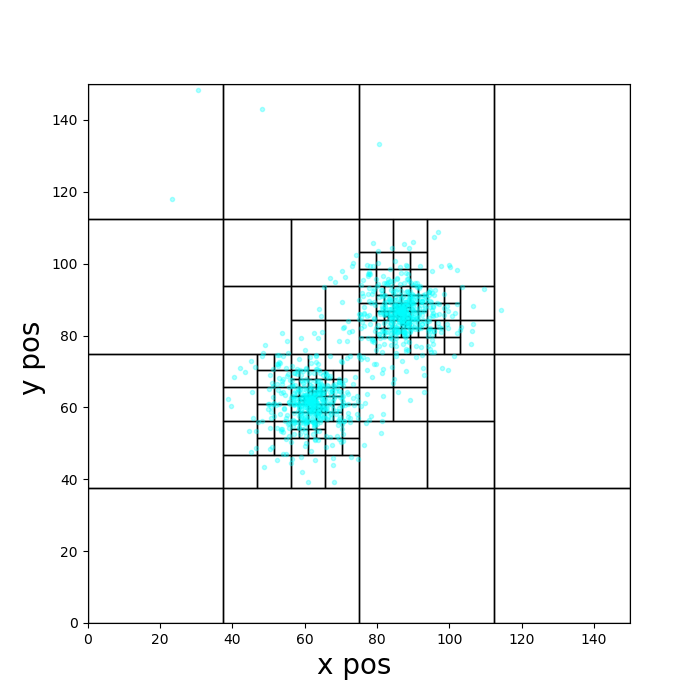
\includegraphics[width=0.9\linewidth]{./plots/quadtree.png}
    \caption{Quadtree plotted.}
    \label{quad}
\end{figure}


\section{Problem 8}
Not implemented. Sad!

Another small rant. I would like it to be known that Computational Astrophysics
is a course based entirely on simulations ($6$ ECs). There were $5$ assignments
that took several weeks to code up---\emph{with} the simulation backbone
already provided (via \texttt{AMUSE}). This problem could probably take a
month to complete on its own. And it is only worth a small fraction of the
final grade. I would love to continue talks on the expectations of this course
in the future.



\end{document}
